% **************************************************************************************************************
% A Classic Thesis Style
% An Homage to The Elements of Typographic Style
%
% Copyright (C) 2015 André Miede http://www.miede.de
%
% If you like the style then I would appreciate a postcard. My address 
% can be found in the file ClassicThesis.pdf. A collection of the 
% postcards I received so far is available online at 
% http://postcards.miede.de
%
% License:
% This program is free software; you can redistribute it and/or modify 
% it under the terms of the GNU General Public License as published by
% the Free Software Foundation; either version 2 of the License, or
% (at your option) any later version.
%
% This program is distributed in the hope that it will be useful,
% but WITHOUT ANY WARRANTY; without even the implied warranty of
% MERCHANTABILITY or FITNESS FOR A PARTICULAR PURPOSE.  See the
% GNU General Public License for more details.
%
% You should have received a copy of the GNU General Public License
% along with this program; see the file COPYING.  If not, write to
% the Free Software Foundation, Inc., 59 Temple Place - Suite 330,
% Boston, MA 02111-1307, USA.
%
% **************************************************************************************************************

\RequirePackage{fix-cm} % fix some latex issues see: http://texdoc.net/texmf-dist/doc/latex/base/fixltx2e.pdf
\documentclass[ twoside,openright,titlepage,numbers=noenddot,headinclude,%1headlines,% letterpaper a4paper
                footinclude=true,cleardoublepage=empty,abstractoff, % <--- obsolete, remove (todo)
                BCOR=15mm,paper=a4,fontsize=11pt,%11pt,a4paper,% 
                british,%
                ]{scrreprt}


%********************************************************************
% Note: Make all your adjustments in here
%************************************	*******************
% ****************************************************************************************************
% classicthesis-config.tex 
% formerly known as loadpackages.sty, classicthesis-ldpkg.sty, and classicthesis-preamble.sty 
% Use it at the beginning of your ClassicThesis.tex, or as a LaTeX Preamble 
% in your ClassicThesis.{tex,lyx} with % ****************************************************************************************************
% classicthesis-config.tex 
% formerly known as loadpackages.sty, classicthesis-ldpkg.sty, and classicthesis-preamble.sty 
% Use it at the beginning of your ClassicThesis.tex, or as a LaTeX Preamble 
% in your ClassicThesis.{tex,lyx} with % ****************************************************************************************************
% classicthesis-config.tex 
% formerly known as loadpackages.sty, classicthesis-ldpkg.sty, and classicthesis-preamble.sty 
% Use it at the beginning of your ClassicThesis.tex, or as a LaTeX Preamble 
% in your ClassicThesis.{tex,lyx} with \input{classicthesis-config}
% ****************************************************************************************************  
% If you like the classicthesis, then I would appreciate a postcard. 
% My address can be found in the file ClassicThesis.pdf. A collection 
% of the postcards I received so far is available online at 
% http://postcards.miede.de
% ****************************************************************************************************


% ****************************************************************************************************
% 0. Set the encoding of your files. UTF-8 is the only sensible encoding nowadays. If you can't read
% äöüßáéçèê∂åëæƒÏ€ then change the encoding setting in your editor, not the line below. If your editor
% does not support utf8 use another editor!
% ****************************************************************************************************
\PassOptionsToPackage{utf8}{inputenc}
	\usepackage{inputenc}

% ****************************************************************************************************
% 1. Configure classicthesis for your needs here, e.g., remove "drafting" below 
% in order to deactivate the time-stamp on the pages
% ****************************************************************************************************
\PassOptionsToPackage{eulerchapternumbers,listings,%drafting,%
					 pdfspacing,dottedtoc,floatperchapter,%linedheaders,%
					 subfig,beramono,eulermath,parts}{classicthesis}                                        
% ********************************************************************
% Available options for classicthesis.sty 
% (see ClassicThesis.pdf for more information):
% drafting
% parts nochapters linedheaders
% eulerchapternumbers beramono eulermath pdfspacing minionprospacing
% tocaligned dottedtoc manychapters
% listings floatperchapter subfig
% ********************************************************************


% ****************************************************************************************************
% 2. Personal data and user ad-hoc commands
% ****************************************************************************************************
\newcommand{\myTitle}{Data integration in the Rail Domain\xspace}
%\newcommand{\mySubtitle}{Big Data on Big Trains\xspace}
\newcommand{\myDegree}{A thesis submitted to the University of Birmingham for the degree of DOCTOR~OF~
PHILOSOPHY\xspace}
\newcommand{\myName}{Christopher Robert Morris\xspace}
\newcommand{\myProf}{Professor Clive Roberts\xspace}
\newcommand{\mySupervisor}{Dr John Easton\xspace}
\newcommand{\myDepartment}{Birmingham Centre for Rail Research and Education\xspace}
\newcommand{\myFaculty}{Electronic, Electrical and Systems Engineering\xspace}
\newcommand{\myUni}{University of Birmingham\xspace}
\newcommand{\myLocation}{Birmingham\xspace}
\newcommand{\myTime}{December 2017\xspace}
%\newcommand{\myVersion}{version 0.2\xspace}

% ********************************************************************
% Setup, finetuning, and useful commands
% ********************************************************************
\newcounter{dummy} % necessary for correct hyperlinks (to index, bib, etc.)
\newlength{\abcd} % for ab..z string length calculation
\providecommand{\mLyX}{L\kern-.1667em\lower.25em\hbox{Y}\kern-.125emX\@}
\newcommand{\ie}{i.\,e.}
\newcommand{\Ie}{I.\,e.}
\newcommand{\eg}{e.\,g.}
\newcommand{\Eg}{E.\,g.} 
% ****************************************************************************************************


% ****************************************************************************************************
% 3. Loading some handy packages
% ****************************************************************************************************
% ******************************************************************** 
% Packages with options that might require adjustments
% ******************************************************************** 
\PassOptionsToPackage{british}{babel}   % change this to your language(s)
% Spanish languages need extra options in order to work with this template
%\PassOptionsToPackage{spanish,es-lcroman}{babel}
	\usepackage{babel}                  

%Jon tutchers ref style
%\usepackage[style=numeric,citestyle=numeric,natbib=true,backend=biber,firstinits=true,isbn=false,sortcites=true,backref=true,url=false,doi=false]{biblatex}


\usepackage{csquotes}
\PassOptionsToPackage{%
    %backend=biber, bibencoding=utf8%instead of bibtex
    backend=bibtex8,bibencoding=utf8,%
    language=auto,%
    %style=alphabetic,%
    %style=numeric-comp,%
    style=authoryear-comp, % Author 1999, 2010
    %bibstyle=authoryear,dashed=false, % dashed: substitute rep. author with ---
    sorting=nyt, % name, year, title
    maxbibnames=2, % default: 3, et al.
    %backref=true,%
    natbib=true % natbib compatibility mode (\citep and \citet still work)
}{biblatex}
    \usepackage{biblatex}


\PassOptionsToPackage{fleqn}{amsmath}       % math environments and more by the AMS 
    \usepackage{amsmath}


% ******************************************************************** 
% General useful packages
% ******************************************************************** 
\PassOptionsToPackage{T1}{fontenc} % T2A for cyrillics
    \usepackage{fontenc}     
\usepackage{textcomp} % fix warning with missing font shapes
\usepackage{scrhack} % fix warnings when using KOMA with listings package          
\usepackage{xspace} % to get the spacing after macros right  
\usepackage{mparhack} % get marginpar right
\usepackage{fixltx2e} % fixes some LaTeX stuff --> since 2015 in the LaTeX kernel (see below)
\usepackage[latest]{latexrelease} % will be used once available in more distributions (ISSUE #107)
%\PassOptionsToPackage{printonlyused,smaller}{acronym} 
    \usepackage{acronym} % nice macros for handling all acronyms in the thesis
    %\renewcommand{\bflabel}[1]{{#1}\hfill} % fix the list of acronyms --> no longer working
    %\renewcommand*{\acsfont}[1]{\textsc{#1}} 
   % \renewcommand*{\aclabelfont}[1]{\acsfont{#1}}
% ****************************************************************************************************


% ****************************************************************************************************
% 4. Setup floats: tables, (sub)figures, and captions
% ****************************************************************************************************
\usepackage{tabularx} % better tables
    \setlength{\extrarowheight}{3pt} % increase table row height
\newcommand{\tableheadline}[1]{\multicolumn{1}{c}{\spacedlowsmallcaps{#1}}}
\newcommand{\myfloatalign}{\centering} % to be used with each float for alignment
\usepackage{caption}
\usepackage[table, svgnames]{xcolor} % because who doesn't like coloured lines in tables?
\newcommand{\mycell}[1]{%
  \begin{tabular}[t]{@{}l@{}} #1 \end{tabular}} % instead of using multirow https://tex.stackexchange.com/questions/404075/tabularx-and-multiple-multirow-cells
% Thanks to cgnieder and Claus Lahiri
% http://tex.stackexchange.com/questions/69349/spacedlowsmallcaps-in-caption-label
% [REMOVED DUE TO OTHER PROBLEMS, SEE ISSUE #82]    
%\DeclareCaptionLabelFormat{smallcaps}{\bothIfFirst{#1}{~}\MakeTextLowercase{\textsc{#2}}}
%\captionsetup{font=small,labelformat=smallcaps} % format=hang,
\captionsetup{font=small} % format=hang,
\usepackage{subfig}  
% ****************************************************************************************************

% *******************************************
% 4.5 My additions
% ******************************************
\usepackage{float} %lets use speficy H for actually here on figures
\usepackage{rotating} %sideways figures
\usepackage{blindtext}
\usepackage{longtable}
\usepackage{tabu}
\usepackage{pdflscape}
\usepackage{fancyref}
\usepackage{dirtytalk}
%Can set max widths or heights on floats
\usepackage[export]{adjustbox} 

% epigraph for massive quotes
\usepackage{epigraph}
%\setlength\epigraphwidth{8cm}
\setlength\epigraphrule{0pt}

%**************************
%Adjust existing commands
%**************************
\usepackage{etoolbox}

\makeatletter
\patchcmd{\epigraph}{\@epitext{#1}}{\itshape\@epitext{#1}}{}{}
\makeatother

\AtBeginEnvironment{quote}{\fontfamily{lmss}\selectfont} %put block quotes in a distinctive font




% ****************************************************************************************************
% 5. Setup code listings
% ****************************************************************************************************
\usepackage{listings} 
\definecolor{codeBackground}{gray}{0.97}
%\lstset{emph={trueIndex,root},emphstyle=\color{BlueViolet}}%\underbar} % for special keywords
\lstset{language=[LaTeX]Tex,%C++,
    backgroundcolor=\color{codeBackground},
    morekeywords={PassOptionsToPackage,selectlanguage},
    keywordstyle=\color{RoyalBlue},%\bfseries,
    basicstyle=\small\ttfamily,
    %identifierstyle=\color{NavyBlue},
    commentstyle=\color{Green}\ttfamily,
    stringstyle=\rmfamily,
    numbers=none,%left,%
    numberstyle=\scriptsize,%\tiny
    stepnumber=5,
    numbersep=8pt,
    showstringspaces=false,
    breaklines=true,
    %frameround=ftff,
    %frame=single,
    belowcaptionskip=.75\baselineskip
    %frame=L
} 
% ****************************************************************************************************             
% ************************
% Code listing styles
% *******************
% Language Definitions for SPARQL

\lstdefinelanguage{XML}
{
  morestring=[b]",
  morestring=[s]{>}{<},
  morecomment=[s]{<?}{?>},
  stringstyle=\color{black},
  identifierstyle=\color{darkblue},
  keywordstyle=\color{cyan},
  morekeywords={xmlns,version,type}% list your attributes here
}

\lstdefinelanguage{sparql}{
morecomment=[l][\color{olivegreen}]{\#},
morestring=[b][\color{purple}]\",
moredelim=[s][\bfseries\color{Maroon}]{<}{\ },
  moredelim=[s][\bfseries\color{Maroon}]{</}{>},
  moredelim=[l][\bfseries\color{Maroon}]{/>},
  moredelim=[l][\bfseries\color{Maroon}]{>},
morekeywords={SELECT,DISTINCT,CONSTRUCT,DESCRIBE,ASK,WHERE,FROM,NAMED,PREFIX,BASE,OPTIONAL,FILTER,GRAPH,LIMIT,OFFSET,SERVICE,UNION,EXISTS,NOT,BINDINGS,MINUS,a},
sensitive=true,
% Variables
    moredelim=*[s][\color{teal}]{?}{\ }
}

% Language Definitions for Turtle
\lstdefinelanguage{turtle}{
alsoletter={-?},
morecomment=[l][\color{olivegreen}]{\#},
morestring=[b][\color{purple}]\",
moredelim=[s][\bfseries\color{Maroon}]{<}{\ },
  moredelim=[s][\bfseries\color{Maroon}]{</}{>},
  moredelim=[l][\bfseries\color{Maroon}]{/>},
  moredelim=[l][\bfseries\color{Maroon}]{>},
morekeywords={@prefix,@base,@forSome,@forAll,@keywords,CONSTRUCT,DESCRIBE,NAMED,PREFIX,BASE,OPTIONAL,FILTER,GRAPH,LIMIT,OFFSET,SERVICE,UNION,EXISTS,NOT,BINDINGS,MINUS,a},
sensitive=true,
% Variables
    moredelim=*[s][\color{teal}]{\#}{\ }
    moredelim=*[2][\color{blue}]{\@}{\ }
}



% ****************************************************************************************************
% 6. PDFLaTeX, hyperreferences and citation backreferences
% ****************************************************************************************************
% ********************************************************************
% Using PDFLaTeX
% ********************************************************************
\PassOptionsToPackage{pdftex,hyperfootnotes=false,pdfpagelabels}{hyperref}
    \usepackage{hyperref}  % backref linktocpage pagebackref
\pdfcompresslevel=9
\pdfadjustspacing=1 
\PassOptionsToPackage{pdftex}{graphicx}
    \usepackage{graphicx} 
 

% ********************************************************************
% Hyperreferences
% ********************************************************************
\hypersetup{%
    %draft, % = no hyperlinking at all (useful in b/w printouts)
    colorlinks=true, linktocpage=false, pdfstartpage=3, pdfstartview=FitH,%Fit verticle, so you can read it more easily
    % uncomment the following line if you want to have black links (e.g., for printing)
    %colorlinks=false, linktocpage=false, pdfstartpage=3, pdfstartview=FitV, pdfborder={0 0 0},%
    breaklinks=true, pdfpagemode=UseNone, pageanchor=true, pdfpagemode=UseOutlines,%
    plainpages=false, bookmarksnumbered, bookmarksopen=true, bookmarksopenlevel=1,%
    hypertexnames=true, pdfhighlight=/O,%nesting=true,%frenchlinks,%
    urlcolor=webbrown, linkcolor=RoyalBlue, citecolor=webgreen, %pagecolor=RoyalBlue,%
    %urlcolor=Black, linkcolor=Black, citecolor=Black, %pagecolor=Black,%
    pdftitle={\myTitle},%
    pdfauthor={\textcopyright\ \myName, \myUni, \myFaculty},%
    pdfsubject={\myTitle},%
    pdfkeywords={Ontology},%
    pdfcreator={pdfLaTeX},%
    pdfproducer={LaTeX with hyperref and classicthesis}%
}   

% ********************************************************************
% Setup autoreferences
% ********************************************************************
% There are some issues regarding autorefnames
% http://www.ureader.de/msg/136221647.aspx
% http://www.tex.ac.uk/cgi-bin/texfaq2html?label=latexwords
% you have to redefine the makros for the 
% language you use, e.g., american, ngerman
% (as chosen when loading babel/AtBeginDocument)
% ********************************************************************
\makeatletter
\@ifpackageloaded{babel}%
    {%
       \addto\extrasenglish{%
			\renewcommand*{\figureautorefname}{Figure}%
			\renewcommand*{\tableautorefname}{Table}%
			\renewcommand*{\partautorefname}{Part}%
			\renewcommand*{\chapterautorefname}{Chapter}%
			\renewcommand*{\sectionautorefname}{Section}%
			\renewcommand*{\subsectionautorefname}{Section}%
			\renewcommand*{\subsubsectionautorefname}{Section}%     
                }%
            % Fix to getting autorefs for subfigures right (thanks to Belinda Vogt for changing the definition)
            \providecommand{\subfigureautorefname}{\figureautorefname}%             
    }{\relax}
\makeatother

% *********************************************************
% Debug only
% ********************************************************
%\usepackage{lua-visual-debug}
% ****************************************************************************************************
% 7. Last calls before the bar closes
% ****************************************************************************************************
% ********************************************************************
% Development Stuff
% ********************************************************************
\listfiles
%\PassOptionsToPackage{l2tabu,orthodox,abort}{nag}
%   \usepackage{nag}
%\PassOptionsToPackage{warning, all}{onlyamsmath}
%   \usepackage{onlyamsmath}

% ********************************************************************
% Last, but not least...
% ********************************************************************
\usepackage{classicthesis} 
% ****************************************************************************************************


% ****************************************************************************************************
% 8. Further adjustments (experimental)
% ****************************************************************************************************
% ********************************************************************
% Changing the text area
% ********************************************************************
%\linespread{1.05} % a bit more for Palatino
%\areaset[current]{312pt}{761pt} % 686 (factor 2.2) + 33 head + 42 head \the\footskip
%\setlength{\marginparwidth}{7em}%
%\setlength{\marginparsep}{2em}%
\usepackage{setspace}
 \setstretch{1.6}
\emergencystretch=.5em


% ********************************************************************
% Using different fonts
% ********************************************************************
%\usepackage[oldstylenums]{kpfonts} % oldstyle notextcomp
%\usepackage[osf]{libertine}
%\usepackage[light,condensed,math]{iwona}
%\renewcommand{\sfdefault}{iwona}
%\usepackage{lmodern} % <-- no osf support :-(
%\usepackage{cfr-lm} % 
%\usepackage[urw-garamond]{mathdesign} <-- no osf support :-(
%\usepackage[default,osfigures]{opensans} % scale=0.95 
%\usepackage[sfdefault]{FiraSans}
% ****************************************************************************************************

% ****************************************************************************************************  
% If you like the classicthesis, then I would appreciate a postcard. 
% My address can be found in the file ClassicThesis.pdf. A collection 
% of the postcards I received so far is available online at 
% http://postcards.miede.de
% ****************************************************************************************************


% ****************************************************************************************************
% 0. Set the encoding of your files. UTF-8 is the only sensible encoding nowadays. If you can't read
% äöüßáéçèê∂åëæƒÏ€ then change the encoding setting in your editor, not the line below. If your editor
% does not support utf8 use another editor!
% ****************************************************************************************************
\PassOptionsToPackage{utf8}{inputenc}
	\usepackage{inputenc}

% ****************************************************************************************************
% 1. Configure classicthesis for your needs here, e.g., remove "drafting" below 
% in order to deactivate the time-stamp on the pages
% ****************************************************************************************************
\PassOptionsToPackage{eulerchapternumbers,listings,%drafting,%
					 pdfspacing,dottedtoc,floatperchapter,%linedheaders,%
					 subfig,beramono,eulermath,parts}{classicthesis}                                        
% ********************************************************************
% Available options for classicthesis.sty 
% (see ClassicThesis.pdf for more information):
% drafting
% parts nochapters linedheaders
% eulerchapternumbers beramono eulermath pdfspacing minionprospacing
% tocaligned dottedtoc manychapters
% listings floatperchapter subfig
% ********************************************************************


% ****************************************************************************************************
% 2. Personal data and user ad-hoc commands
% ****************************************************************************************************
\newcommand{\myTitle}{Data integration in the Rail Domain\xspace}
%\newcommand{\mySubtitle}{Big Data on Big Trains\xspace}
\newcommand{\myDegree}{A thesis submitted to the University of Birmingham for the degree of DOCTOR~OF~
PHILOSOPHY\xspace}
\newcommand{\myName}{Christopher Robert Morris\xspace}
\newcommand{\myProf}{Professor Clive Roberts\xspace}
\newcommand{\mySupervisor}{Dr John Easton\xspace}
\newcommand{\myDepartment}{Birmingham Centre for Rail Research and Education\xspace}
\newcommand{\myFaculty}{Electronic, Electrical and Systems Engineering\xspace}
\newcommand{\myUni}{University of Birmingham\xspace}
\newcommand{\myLocation}{Birmingham\xspace}
\newcommand{\myTime}{December 2017\xspace}
%\newcommand{\myVersion}{version 0.2\xspace}

% ********************************************************************
% Setup, finetuning, and useful commands
% ********************************************************************
\newcounter{dummy} % necessary for correct hyperlinks (to index, bib, etc.)
\newlength{\abcd} % for ab..z string length calculation
\providecommand{\mLyX}{L\kern-.1667em\lower.25em\hbox{Y}\kern-.125emX\@}
\newcommand{\ie}{i.\,e.}
\newcommand{\Ie}{I.\,e.}
\newcommand{\eg}{e.\,g.}
\newcommand{\Eg}{E.\,g.} 
% ****************************************************************************************************


% ****************************************************************************************************
% 3. Loading some handy packages
% ****************************************************************************************************
% ******************************************************************** 
% Packages with options that might require adjustments
% ******************************************************************** 
\PassOptionsToPackage{british}{babel}   % change this to your language(s)
% Spanish languages need extra options in order to work with this template
%\PassOptionsToPackage{spanish,es-lcroman}{babel}
	\usepackage{babel}                  

%Jon tutchers ref style
%\usepackage[style=numeric,citestyle=numeric,natbib=true,backend=biber,firstinits=true,isbn=false,sortcites=true,backref=true,url=false,doi=false]{biblatex}


\usepackage{csquotes}
\PassOptionsToPackage{%
    %backend=biber, bibencoding=utf8%instead of bibtex
    backend=bibtex8,bibencoding=utf8,%
    language=auto,%
    %style=alphabetic,%
    %style=numeric-comp,%
    style=authoryear-comp, % Author 1999, 2010
    %bibstyle=authoryear,dashed=false, % dashed: substitute rep. author with ---
    sorting=nyt, % name, year, title
    maxbibnames=2, % default: 3, et al.
    %backref=true,%
    natbib=true % natbib compatibility mode (\citep and \citet still work)
}{biblatex}
    \usepackage{biblatex}


\PassOptionsToPackage{fleqn}{amsmath}       % math environments and more by the AMS 
    \usepackage{amsmath}


% ******************************************************************** 
% General useful packages
% ******************************************************************** 
\PassOptionsToPackage{T1}{fontenc} % T2A for cyrillics
    \usepackage{fontenc}     
\usepackage{textcomp} % fix warning with missing font shapes
\usepackage{scrhack} % fix warnings when using KOMA with listings package          
\usepackage{xspace} % to get the spacing after macros right  
\usepackage{mparhack} % get marginpar right
\usepackage{fixltx2e} % fixes some LaTeX stuff --> since 2015 in the LaTeX kernel (see below)
\usepackage[latest]{latexrelease} % will be used once available in more distributions (ISSUE #107)
%\PassOptionsToPackage{printonlyused,smaller}{acronym} 
    \usepackage{acronym} % nice macros for handling all acronyms in the thesis
    %\renewcommand{\bflabel}[1]{{#1}\hfill} % fix the list of acronyms --> no longer working
    %\renewcommand*{\acsfont}[1]{\textsc{#1}} 
   % \renewcommand*{\aclabelfont}[1]{\acsfont{#1}}
% ****************************************************************************************************


% ****************************************************************************************************
% 4. Setup floats: tables, (sub)figures, and captions
% ****************************************************************************************************
\usepackage{tabularx} % better tables
    \setlength{\extrarowheight}{3pt} % increase table row height
\newcommand{\tableheadline}[1]{\multicolumn{1}{c}{\spacedlowsmallcaps{#1}}}
\newcommand{\myfloatalign}{\centering} % to be used with each float for alignment
\usepackage{caption}
\usepackage[table, svgnames]{xcolor} % because who doesn't like coloured lines in tables?
\newcommand{\mycell}[1]{%
  \begin{tabular}[t]{@{}l@{}} #1 \end{tabular}} % instead of using multirow https://tex.stackexchange.com/questions/404075/tabularx-and-multiple-multirow-cells
% Thanks to cgnieder and Claus Lahiri
% http://tex.stackexchange.com/questions/69349/spacedlowsmallcaps-in-caption-label
% [REMOVED DUE TO OTHER PROBLEMS, SEE ISSUE #82]    
%\DeclareCaptionLabelFormat{smallcaps}{\bothIfFirst{#1}{~}\MakeTextLowercase{\textsc{#2}}}
%\captionsetup{font=small,labelformat=smallcaps} % format=hang,
\captionsetup{font=small} % format=hang,
\usepackage{subfig}  
% ****************************************************************************************************

% *******************************************
% 4.5 My additions
% ******************************************
\usepackage{float} %lets use speficy H for actually here on figures
\usepackage{rotating} %sideways figures
\usepackage{blindtext}
\usepackage{longtable}
\usepackage{tabu}
\usepackage{pdflscape}
\usepackage{fancyref}
\usepackage{dirtytalk}
%Can set max widths or heights on floats
\usepackage[export]{adjustbox} 

% epigraph for massive quotes
\usepackage{epigraph}
%\setlength\epigraphwidth{8cm}
\setlength\epigraphrule{0pt}

%**************************
%Adjust existing commands
%**************************
\usepackage{etoolbox}

\makeatletter
\patchcmd{\epigraph}{\@epitext{#1}}{\itshape\@epitext{#1}}{}{}
\makeatother

\AtBeginEnvironment{quote}{\fontfamily{lmss}\selectfont} %put block quotes in a distinctive font




% ****************************************************************************************************
% 5. Setup code listings
% ****************************************************************************************************
\usepackage{listings} 
\definecolor{codeBackground}{gray}{0.97}
%\lstset{emph={trueIndex,root},emphstyle=\color{BlueViolet}}%\underbar} % for special keywords
\lstset{language=[LaTeX]Tex,%C++,
    backgroundcolor=\color{codeBackground},
    morekeywords={PassOptionsToPackage,selectlanguage},
    keywordstyle=\color{RoyalBlue},%\bfseries,
    basicstyle=\small\ttfamily,
    %identifierstyle=\color{NavyBlue},
    commentstyle=\color{Green}\ttfamily,
    stringstyle=\rmfamily,
    numbers=none,%left,%
    numberstyle=\scriptsize,%\tiny
    stepnumber=5,
    numbersep=8pt,
    showstringspaces=false,
    breaklines=true,
    %frameround=ftff,
    %frame=single,
    belowcaptionskip=.75\baselineskip
    %frame=L
} 
% ****************************************************************************************************             
% ************************
% Code listing styles
% *******************
% Language Definitions for SPARQL

\lstdefinelanguage{XML}
{
  morestring=[b]",
  morestring=[s]{>}{<},
  morecomment=[s]{<?}{?>},
  stringstyle=\color{black},
  identifierstyle=\color{darkblue},
  keywordstyle=\color{cyan},
  morekeywords={xmlns,version,type}% list your attributes here
}

\lstdefinelanguage{sparql}{
morecomment=[l][\color{olivegreen}]{\#},
morestring=[b][\color{purple}]\",
moredelim=[s][\bfseries\color{Maroon}]{<}{\ },
  moredelim=[s][\bfseries\color{Maroon}]{</}{>},
  moredelim=[l][\bfseries\color{Maroon}]{/>},
  moredelim=[l][\bfseries\color{Maroon}]{>},
morekeywords={SELECT,DISTINCT,CONSTRUCT,DESCRIBE,ASK,WHERE,FROM,NAMED,PREFIX,BASE,OPTIONAL,FILTER,GRAPH,LIMIT,OFFSET,SERVICE,UNION,EXISTS,NOT,BINDINGS,MINUS,a},
sensitive=true,
% Variables
    moredelim=*[s][\color{teal}]{?}{\ }
}

% Language Definitions for Turtle
\lstdefinelanguage{turtle}{
alsoletter={-?},
morecomment=[l][\color{olivegreen}]{\#},
morestring=[b][\color{purple}]\",
moredelim=[s][\bfseries\color{Maroon}]{<}{\ },
  moredelim=[s][\bfseries\color{Maroon}]{</}{>},
  moredelim=[l][\bfseries\color{Maroon}]{/>},
  moredelim=[l][\bfseries\color{Maroon}]{>},
morekeywords={@prefix,@base,@forSome,@forAll,@keywords,CONSTRUCT,DESCRIBE,NAMED,PREFIX,BASE,OPTIONAL,FILTER,GRAPH,LIMIT,OFFSET,SERVICE,UNION,EXISTS,NOT,BINDINGS,MINUS,a},
sensitive=true,
% Variables
    moredelim=*[s][\color{teal}]{\#}{\ }
    moredelim=*[2][\color{blue}]{\@}{\ }
}



% ****************************************************************************************************
% 6. PDFLaTeX, hyperreferences and citation backreferences
% ****************************************************************************************************
% ********************************************************************
% Using PDFLaTeX
% ********************************************************************
\PassOptionsToPackage{pdftex,hyperfootnotes=false,pdfpagelabels}{hyperref}
    \usepackage{hyperref}  % backref linktocpage pagebackref
\pdfcompresslevel=9
\pdfadjustspacing=1 
\PassOptionsToPackage{pdftex}{graphicx}
    \usepackage{graphicx} 
 

% ********************************************************************
% Hyperreferences
% ********************************************************************
\hypersetup{%
    %draft, % = no hyperlinking at all (useful in b/w printouts)
    colorlinks=true, linktocpage=false, pdfstartpage=3, pdfstartview=FitH,%Fit verticle, so you can read it more easily
    % uncomment the following line if you want to have black links (e.g., for printing)
    %colorlinks=false, linktocpage=false, pdfstartpage=3, pdfstartview=FitV, pdfborder={0 0 0},%
    breaklinks=true, pdfpagemode=UseNone, pageanchor=true, pdfpagemode=UseOutlines,%
    plainpages=false, bookmarksnumbered, bookmarksopen=true, bookmarksopenlevel=1,%
    hypertexnames=true, pdfhighlight=/O,%nesting=true,%frenchlinks,%
    urlcolor=webbrown, linkcolor=RoyalBlue, citecolor=webgreen, %pagecolor=RoyalBlue,%
    %urlcolor=Black, linkcolor=Black, citecolor=Black, %pagecolor=Black,%
    pdftitle={\myTitle},%
    pdfauthor={\textcopyright\ \myName, \myUni, \myFaculty},%
    pdfsubject={\myTitle},%
    pdfkeywords={Ontology},%
    pdfcreator={pdfLaTeX},%
    pdfproducer={LaTeX with hyperref and classicthesis}%
}   

% ********************************************************************
% Setup autoreferences
% ********************************************************************
% There are some issues regarding autorefnames
% http://www.ureader.de/msg/136221647.aspx
% http://www.tex.ac.uk/cgi-bin/texfaq2html?label=latexwords
% you have to redefine the makros for the 
% language you use, e.g., american, ngerman
% (as chosen when loading babel/AtBeginDocument)
% ********************************************************************
\makeatletter
\@ifpackageloaded{babel}%
    {%
       \addto\extrasenglish{%
			\renewcommand*{\figureautorefname}{Figure}%
			\renewcommand*{\tableautorefname}{Table}%
			\renewcommand*{\partautorefname}{Part}%
			\renewcommand*{\chapterautorefname}{Chapter}%
			\renewcommand*{\sectionautorefname}{Section}%
			\renewcommand*{\subsectionautorefname}{Section}%
			\renewcommand*{\subsubsectionautorefname}{Section}%     
                }%
            % Fix to getting autorefs for subfigures right (thanks to Belinda Vogt for changing the definition)
            \providecommand{\subfigureautorefname}{\figureautorefname}%             
    }{\relax}
\makeatother

% *********************************************************
% Debug only
% ********************************************************
%\usepackage{lua-visual-debug}
% ****************************************************************************************************
% 7. Last calls before the bar closes
% ****************************************************************************************************
% ********************************************************************
% Development Stuff
% ********************************************************************
\listfiles
%\PassOptionsToPackage{l2tabu,orthodox,abort}{nag}
%   \usepackage{nag}
%\PassOptionsToPackage{warning, all}{onlyamsmath}
%   \usepackage{onlyamsmath}

% ********************************************************************
% Last, but not least...
% ********************************************************************
\usepackage{classicthesis} 
% ****************************************************************************************************


% ****************************************************************************************************
% 8. Further adjustments (experimental)
% ****************************************************************************************************
% ********************************************************************
% Changing the text area
% ********************************************************************
%\linespread{1.05} % a bit more for Palatino
%\areaset[current]{312pt}{761pt} % 686 (factor 2.2) + 33 head + 42 head \the\footskip
%\setlength{\marginparwidth}{7em}%
%\setlength{\marginparsep}{2em}%
\usepackage{setspace}
 \setstretch{1.6}
\emergencystretch=.5em


% ********************************************************************
% Using different fonts
% ********************************************************************
%\usepackage[oldstylenums]{kpfonts} % oldstyle notextcomp
%\usepackage[osf]{libertine}
%\usepackage[light,condensed,math]{iwona}
%\renewcommand{\sfdefault}{iwona}
%\usepackage{lmodern} % <-- no osf support :-(
%\usepackage{cfr-lm} % 
%\usepackage[urw-garamond]{mathdesign} <-- no osf support :-(
%\usepackage[default,osfigures]{opensans} % scale=0.95 
%\usepackage[sfdefault]{FiraSans}
% ****************************************************************************************************

% ****************************************************************************************************  
% If you like the classicthesis, then I would appreciate a postcard. 
% My address can be found in the file ClassicThesis.pdf. A collection 
% of the postcards I received so far is available online at 
% http://postcards.miede.de
% ****************************************************************************************************


% ****************************************************************************************************
% 0. Set the encoding of your files. UTF-8 is the only sensible encoding nowadays. If you can't read
% äöüßáéçèê∂åëæƒÏ€ then change the encoding setting in your editor, not the line below. If your editor
% does not support utf8 use another editor!
% ****************************************************************************************************
\PassOptionsToPackage{utf8}{inputenc}
	\usepackage{inputenc}

% ****************************************************************************************************
% 1. Configure classicthesis for your needs here, e.g., remove "drafting" below 
% in order to deactivate the time-stamp on the pages
% ****************************************************************************************************
\PassOptionsToPackage{eulerchapternumbers,listings,%drafting,%
					 pdfspacing,dottedtoc,floatperchapter,%linedheaders,%
					 subfig,beramono,eulermath,parts}{classicthesis}                                        
% ********************************************************************
% Available options for classicthesis.sty 
% (see ClassicThesis.pdf for more information):
% drafting
% parts nochapters linedheaders
% eulerchapternumbers beramono eulermath pdfspacing minionprospacing
% tocaligned dottedtoc manychapters
% listings floatperchapter subfig
% ********************************************************************


% ****************************************************************************************************
% 2. Personal data and user ad-hoc commands
% ****************************************************************************************************
\newcommand{\myTitle}{Data integration in the Rail Domain\xspace}
%\newcommand{\mySubtitle}{Big Data on Big Trains\xspace}
\newcommand{\myDegree}{A thesis submitted to the University of Birmingham for the degree of DOCTOR~OF~
PHILOSOPHY\xspace}
\newcommand{\myName}{Christopher Robert Morris\xspace}
\newcommand{\myProf}{Professor Clive Roberts\xspace}
\newcommand{\mySupervisor}{Dr John Easton\xspace}
\newcommand{\myDepartment}{Birmingham Centre for Rail Research and Education\xspace}
\newcommand{\myFaculty}{Electronic, Electrical and Systems Engineering\xspace}
\newcommand{\myUni}{University of Birmingham\xspace}
\newcommand{\myLocation}{Birmingham\xspace}
\newcommand{\myTime}{December 2017\xspace}
%\newcommand{\myVersion}{version 0.2\xspace}

% ********************************************************************
% Setup, finetuning, and useful commands
% ********************************************************************
\newcounter{dummy} % necessary for correct hyperlinks (to index, bib, etc.)
\newlength{\abcd} % for ab..z string length calculation
\providecommand{\mLyX}{L\kern-.1667em\lower.25em\hbox{Y}\kern-.125emX\@}
\newcommand{\ie}{i.\,e.}
\newcommand{\Ie}{I.\,e.}
\newcommand{\eg}{e.\,g.}
\newcommand{\Eg}{E.\,g.} 
% ****************************************************************************************************


% ****************************************************************************************************
% 3. Loading some handy packages
% ****************************************************************************************************
% ******************************************************************** 
% Packages with options that might require adjustments
% ******************************************************************** 
\PassOptionsToPackage{british}{babel}   % change this to your language(s)
% Spanish languages need extra options in order to work with this template
%\PassOptionsToPackage{spanish,es-lcroman}{babel}
	\usepackage{babel}                  

%Jon tutchers ref style
%\usepackage[style=numeric,citestyle=numeric,natbib=true,backend=biber,firstinits=true,isbn=false,sortcites=true,backref=true,url=false,doi=false]{biblatex}


\usepackage{csquotes}
\PassOptionsToPackage{%
    %backend=biber, bibencoding=utf8%instead of bibtex
    backend=bibtex8,bibencoding=utf8,%
    language=auto,%
    %style=alphabetic,%
    %style=numeric-comp,%
    style=authoryear-comp, % Author 1999, 2010
    %bibstyle=authoryear,dashed=false, % dashed: substitute rep. author with ---
    sorting=nyt, % name, year, title
    maxbibnames=2, % default: 3, et al.
    %backref=true,%
    natbib=true % natbib compatibility mode (\citep and \citet still work)
}{biblatex}
    \usepackage{biblatex}


\PassOptionsToPackage{fleqn}{amsmath}       % math environments and more by the AMS 
    \usepackage{amsmath}


% ******************************************************************** 
% General useful packages
% ******************************************************************** 
\PassOptionsToPackage{T1}{fontenc} % T2A for cyrillics
    \usepackage{fontenc}     
\usepackage{textcomp} % fix warning with missing font shapes
\usepackage{scrhack} % fix warnings when using KOMA with listings package          
\usepackage{xspace} % to get the spacing after macros right  
\usepackage{mparhack} % get marginpar right
\usepackage{fixltx2e} % fixes some LaTeX stuff --> since 2015 in the LaTeX kernel (see below)
\usepackage[latest]{latexrelease} % will be used once available in more distributions (ISSUE #107)
%\PassOptionsToPackage{printonlyused,smaller}{acronym} 
    \usepackage{acronym} % nice macros for handling all acronyms in the thesis
    %\renewcommand{\bflabel}[1]{{#1}\hfill} % fix the list of acronyms --> no longer working
    %\renewcommand*{\acsfont}[1]{\textsc{#1}} 
   % \renewcommand*{\aclabelfont}[1]{\acsfont{#1}}
% ****************************************************************************************************


% ****************************************************************************************************
% 4. Setup floats: tables, (sub)figures, and captions
% ****************************************************************************************************
\usepackage{tabularx} % better tables
    \setlength{\extrarowheight}{3pt} % increase table row height
\newcommand{\tableheadline}[1]{\multicolumn{1}{c}{\spacedlowsmallcaps{#1}}}
\newcommand{\myfloatalign}{\centering} % to be used with each float for alignment
\usepackage{caption}
\usepackage[table, svgnames]{xcolor} % because who doesn't like coloured lines in tables?
\newcommand{\mycell}[1]{%
  \begin{tabular}[t]{@{}l@{}} #1 \end{tabular}} % instead of using multirow https://tex.stackexchange.com/questions/404075/tabularx-and-multiple-multirow-cells
% Thanks to cgnieder and Claus Lahiri
% http://tex.stackexchange.com/questions/69349/spacedlowsmallcaps-in-caption-label
% [REMOVED DUE TO OTHER PROBLEMS, SEE ISSUE #82]    
%\DeclareCaptionLabelFormat{smallcaps}{\bothIfFirst{#1}{~}\MakeTextLowercase{\textsc{#2}}}
%\captionsetup{font=small,labelformat=smallcaps} % format=hang,
\captionsetup{font=small} % format=hang,
\usepackage{subfig}  
% ****************************************************************************************************

% *******************************************
% 4.5 My additions
% ******************************************
\usepackage{float} %lets use speficy H for actually here on figures
\usepackage{rotating} %sideways figures
\usepackage{blindtext}
\usepackage{longtable}
\usepackage{tabu}
\usepackage{pdflscape}
\usepackage{fancyref}
\usepackage{dirtytalk}
%Can set max widths or heights on floats
\usepackage[export]{adjustbox} 

% epigraph for massive quotes
\usepackage{epigraph}
%\setlength\epigraphwidth{8cm}
\setlength\epigraphrule{0pt}

%**************************
%Adjust existing commands
%**************************
\usepackage{etoolbox}

\makeatletter
\patchcmd{\epigraph}{\@epitext{#1}}{\itshape\@epitext{#1}}{}{}
\makeatother

\AtBeginEnvironment{quote}{\fontfamily{lmss}\selectfont} %put block quotes in a distinctive font




% ****************************************************************************************************
% 5. Setup code listings
% ****************************************************************************************************
\usepackage{listings} 
\definecolor{codeBackground}{gray}{0.97}
%\lstset{emph={trueIndex,root},emphstyle=\color{BlueViolet}}%\underbar} % for special keywords
\lstset{language=[LaTeX]Tex,%C++,
    backgroundcolor=\color{codeBackground},
    morekeywords={PassOptionsToPackage,selectlanguage},
    keywordstyle=\color{RoyalBlue},%\bfseries,
    basicstyle=\small\ttfamily,
    %identifierstyle=\color{NavyBlue},
    commentstyle=\color{Green}\ttfamily,
    stringstyle=\rmfamily,
    numbers=none,%left,%
    numberstyle=\scriptsize,%\tiny
    stepnumber=5,
    numbersep=8pt,
    showstringspaces=false,
    breaklines=true,
    %frameround=ftff,
    %frame=single,
    belowcaptionskip=.75\baselineskip
    %frame=L
} 
% ****************************************************************************************************             
% ************************
% Code listing styles
% *******************
% Language Definitions for SPARQL

\lstdefinelanguage{XML}
{
  morestring=[b]",
  morestring=[s]{>}{<},
  morecomment=[s]{<?}{?>},
  stringstyle=\color{black},
  identifierstyle=\color{darkblue},
  keywordstyle=\color{cyan},
  morekeywords={xmlns,version,type}% list your attributes here
}

\lstdefinelanguage{sparql}{
morecomment=[l][\color{olivegreen}]{\#},
morestring=[b][\color{purple}]\",
moredelim=[s][\bfseries\color{Maroon}]{<}{\ },
  moredelim=[s][\bfseries\color{Maroon}]{</}{>},
  moredelim=[l][\bfseries\color{Maroon}]{/>},
  moredelim=[l][\bfseries\color{Maroon}]{>},
morekeywords={SELECT,DISTINCT,CONSTRUCT,DESCRIBE,ASK,WHERE,FROM,NAMED,PREFIX,BASE,OPTIONAL,FILTER,GRAPH,LIMIT,OFFSET,SERVICE,UNION,EXISTS,NOT,BINDINGS,MINUS,a},
sensitive=true,
% Variables
    moredelim=*[s][\color{teal}]{?}{\ }
}

% Language Definitions for Turtle
\lstdefinelanguage{turtle}{
alsoletter={-?},
morecomment=[l][\color{olivegreen}]{\#},
morestring=[b][\color{purple}]\",
moredelim=[s][\bfseries\color{Maroon}]{<}{\ },
  moredelim=[s][\bfseries\color{Maroon}]{</}{>},
  moredelim=[l][\bfseries\color{Maroon}]{/>},
  moredelim=[l][\bfseries\color{Maroon}]{>},
morekeywords={@prefix,@base,@forSome,@forAll,@keywords,CONSTRUCT,DESCRIBE,NAMED,PREFIX,BASE,OPTIONAL,FILTER,GRAPH,LIMIT,OFFSET,SERVICE,UNION,EXISTS,NOT,BINDINGS,MINUS,a},
sensitive=true,
% Variables
    moredelim=*[s][\color{teal}]{\#}{\ }
    moredelim=*[2][\color{blue}]{\@}{\ }
}



% ****************************************************************************************************
% 6. PDFLaTeX, hyperreferences and citation backreferences
% ****************************************************************************************************
% ********************************************************************
% Using PDFLaTeX
% ********************************************************************
\PassOptionsToPackage{pdftex,hyperfootnotes=false,pdfpagelabels}{hyperref}
    \usepackage{hyperref}  % backref linktocpage pagebackref
\pdfcompresslevel=9
\pdfadjustspacing=1 
\PassOptionsToPackage{pdftex}{graphicx}
    \usepackage{graphicx} 
 

% ********************************************************************
% Hyperreferences
% ********************************************************************
\hypersetup{%
    %draft, % = no hyperlinking at all (useful in b/w printouts)
    colorlinks=true, linktocpage=false, pdfstartpage=3, pdfstartview=FitH,%Fit verticle, so you can read it more easily
    % uncomment the following line if you want to have black links (e.g., for printing)
    %colorlinks=false, linktocpage=false, pdfstartpage=3, pdfstartview=FitV, pdfborder={0 0 0},%
    breaklinks=true, pdfpagemode=UseNone, pageanchor=true, pdfpagemode=UseOutlines,%
    plainpages=false, bookmarksnumbered, bookmarksopen=true, bookmarksopenlevel=1,%
    hypertexnames=true, pdfhighlight=/O,%nesting=true,%frenchlinks,%
    urlcolor=webbrown, linkcolor=RoyalBlue, citecolor=webgreen, %pagecolor=RoyalBlue,%
    %urlcolor=Black, linkcolor=Black, citecolor=Black, %pagecolor=Black,%
    pdftitle={\myTitle},%
    pdfauthor={\textcopyright\ \myName, \myUni, \myFaculty},%
    pdfsubject={\myTitle},%
    pdfkeywords={Ontology},%
    pdfcreator={pdfLaTeX},%
    pdfproducer={LaTeX with hyperref and classicthesis}%
}   

% ********************************************************************
% Setup autoreferences
% ********************************************************************
% There are some issues regarding autorefnames
% http://www.ureader.de/msg/136221647.aspx
% http://www.tex.ac.uk/cgi-bin/texfaq2html?label=latexwords
% you have to redefine the makros for the 
% language you use, e.g., american, ngerman
% (as chosen when loading babel/AtBeginDocument)
% ********************************************************************
\makeatletter
\@ifpackageloaded{babel}%
    {%
       \addto\extrasenglish{%
			\renewcommand*{\figureautorefname}{Figure}%
			\renewcommand*{\tableautorefname}{Table}%
			\renewcommand*{\partautorefname}{Part}%
			\renewcommand*{\chapterautorefname}{Chapter}%
			\renewcommand*{\sectionautorefname}{Section}%
			\renewcommand*{\subsectionautorefname}{Section}%
			\renewcommand*{\subsubsectionautorefname}{Section}%     
                }%
            % Fix to getting autorefs for subfigures right (thanks to Belinda Vogt for changing the definition)
            \providecommand{\subfigureautorefname}{\figureautorefname}%             
    }{\relax}
\makeatother

% *********************************************************
% Debug only
% ********************************************************
%\usepackage{lua-visual-debug}
% ****************************************************************************************************
% 7. Last calls before the bar closes
% ****************************************************************************************************
% ********************************************************************
% Development Stuff
% ********************************************************************
\listfiles
%\PassOptionsToPackage{l2tabu,orthodox,abort}{nag}
%   \usepackage{nag}
%\PassOptionsToPackage{warning, all}{onlyamsmath}
%   \usepackage{onlyamsmath}

% ********************************************************************
% Last, but not least...
% ********************************************************************
\usepackage{classicthesis} 
% ****************************************************************************************************


% ****************************************************************************************************
% 8. Further adjustments (experimental)
% ****************************************************************************************************
% ********************************************************************
% Changing the text area
% ********************************************************************
%\linespread{1.05} % a bit more for Palatino
%\areaset[current]{312pt}{761pt} % 686 (factor 2.2) + 33 head + 42 head \the\footskip
%\setlength{\marginparwidth}{7em}%
%\setlength{\marginparsep}{2em}%
\usepackage{setspace}
 \setstretch{1.6}
\emergencystretch=.5em


% ********************************************************************
% Using different fonts
% ********************************************************************
%\usepackage[oldstylenums]{kpfonts} % oldstyle notextcomp
%\usepackage[osf]{libertine}
%\usepackage[light,condensed,math]{iwona}
%\renewcommand{\sfdefault}{iwona}
%\usepackage{lmodern} % <-- no osf support :-(
%\usepackage{cfr-lm} % 
%\usepackage[urw-garamond]{mathdesign} <-- no osf support :-(
%\usepackage[default,osfigures]{opensans} % scale=0.95 
%\usepackage[sfdefault]{FiraSans}
% ****************************************************************************************************


%********************************************************************
% Bibliographies
%*******************************************s************
%\addbibresource{Bibliography.bib}
\addbibresource{library.bib}
%\addbibresource[label=ownpubs]{AMiede_Publications.bib}

%********************************************************************
% Hyphenation
%*******************************************************
%\hyphenation{put special hyphenation here}

%*****************************
%Macros for things that get repeated and might change
%*********************************
\def\QuestionOtherData{Given the diverse information environment within the rail industry, how can heterogeneous datasources be combined, where there is value in so doing?}
\def\QuestionChange{Can an intermediary layer isolate information systems from changes to datastore interfaces?}
\def\QuestionSecurity{How can datastore security be managed within the setting of an ontology and IT infrastructure?}
\def\QuestionCombine{Given that many stakeholders can benefit from combining multiple data sources, what techniques enable this?}
\def\QuestionSkillz{Given the current shortage of engineers with experience editing or connecting to ontologies, is it possible to create tools which improve their uptake and adoption?}
\def\QuestionCanOntologyScale{Given the velocity and volume of data within the rail domain, can an ontology based architecture be deployed on the scale of a national rail network?}


% ********************************************************************
% GO!GO!GO! MOVE IT!
%*******************************************************
\begin{document}
\frenchspacing
\raggedbottom
\selectlanguage{british} % 
%\renewcommand*{\bibname}{new name}
%\setbibpreamble{}
\pagenumbering{roman}
\pagestyle{plain}
%********************************************************************
% Frontmatter
%*******************************************************
%%*******************************************************
% Little Dirty Titlepage
%*******************************************************
\thispagestyle{empty}
%\pdfbookmark[1]{Titel}{title}
%*******************************************************
\begin{center}
    \spacedlowsmallcaps{\myName} \\ \medskip                        

    \begingroup
        \color{Maroon}\spacedallcaps{\myTitle}
    \endgroup
\end{center}        

%*******************************************************
% Titlepage
%*******************************************************
\begin{titlepage}
    % if you want the titlepage to be centered, uncomment and fine-tune the line below (KOMA classes environment)
    %\begin{addmargin}[-1cm]{-3cm}
    %\begin{center}
    \begingroup
        \color{Maroon}\spacedallcaps{\myTitle} \\ \bigskip
    \endgroup

    by \\ \bigskip

    \spacedlowsmallcaps{\myName} \\ \bigskip

    \myDegree

    \vfill
    \bigskip

    \hfill

    \vfill
    \begin{flushright}
        \myDepartment \\                            
        \myFaculty \\
        \myUni  \\
        \myTime \\
    \end{flushright}

       

        %\mySubtitle \\ \medskip   
      %  \myDegree \\ \bigskip

        %\myDepartment \\                            
       % \myFaculty \\
        %\myUni \\ %\bigskip

        %\myTime\ %-- \myVersion

        %\vfill                      

    %\end{center}  
  %\end{addmargin}       
\end{titlepage}   
\thispagestyle{empty}

\hfill

\vfill

\noindent\myName: \textit{\myTitle,} \\ 
\myDegree  %\mySubtitle, %\myDegree, 
\textcopyright\ \myTime

\bigskip

\noindent\spacedlowsmallcaps{Supervisor}: \\
%\myProf \\
%\myOtherProf \\ 
\mySupervisor
%
%\medskip
%
%\noindent\spacedlowsmallcaps{Location}: \\
%\myLocation
%
%\medskip
%
%\noindent\spacedlowsmallcaps{Time Frame}: \\
%\myTime

%\cleardoublepage%*******************************************************
% Dedication
%*******************************************************
\thispagestyle{empty}
%\phantomsection 
\refstepcounter{dummy}
\pdfbookmark[1]{Dedication}{Dedication}

\vspace*{3cm}

\begin{center}
    \emph{Ohana} means family. \\
    Family means nobody gets left behind, or forgotten. \\ \medskip
    --- Lilo \& Stitch    
\end{center}

\medskip

\begin{center}
    Dedicated to the loving memory of Rudolf Miede. \\ \smallskip
    1939\,--\,2005
\end{center}
%\cleardoublepage\include{FrontBackmatter/Foreword} 

\cleardoublepage%*******************************************************
% Abstract
%*******************************************************
%\renewcommand{\abstractname}{Abstract}
\pdfbookmark[1]{Abstract}{Abstract}
\begingroup
\let\clearpage\relax
\let\cleardoublepage\relax
\let\cleardoublepage\relax

\chapter*{Abstract}
The exchange of information is crucial to the operation of railways; starting with the distribution of timetables, information must constantly be exchanged in any railway network. The slow evolution of the information environment within the rail industry has resulted in the existence of a diverse range of systems, only able to exchange information essential to railway operations. Were the cost of data integration reduced, then further cost reductions would follow as barriers to the adoption of other technologies are removed. 

Using linked data and ontology to achieve integration has many advantages over other less information-rich and more prescriptive formats; for example by using a linked data architecture it is possible for anyone to make data available to the industry. Another key advantage of ontology and linked data over other formats for interchange is that it is possible to exchange not merely information, but the logic by which the industry operates. 

The need for data integration has already been studied extensively and has been included in the UK industry's rail technical strategy, however uptake of ontology remains limited. This thesis considers means of reducing barriers to the take up of ontology in the UK rail industry.

\endgroup			

\vfill
%\cleardoublepage%*******************************************************
% Publications
%*******************************************************
\pdfbookmark[1]{Publications}{publications}
\chapter*{Publications}\graffito{This is just an early --~and currently ugly~-- test!}
This might come in handy for PhD theses: some ideas and figures have appeared previously in the following publications:

%\noindent Put your publications from the thesis here. The packages \texttt{multibib} or \texttt{bibtopic} etc. can be used to handle multiple different bibliographies in your document.

\begin{refsection}[ownpubs]
    \small
    \nocite{*} % is local to to the enclosing refsection
    \printbibliography[heading=none]
\end{refsection}

\emph{Attention}: This requires a separate run of \texttt{bibtex} for your \texttt{refsection}, \eg, \texttt{ClassicThesis1-blx} for this file. You might also use \texttt{biber} as the backend for \texttt{biblatex}. See also \url{http://tex.stackexchange.com/questions/128196/problem-with-refsection}.
\cleardoublepage%*******************************************************
% Acknowledgments
%*******************************************************
\pdfbookmark[1]{Acknowledgements}{Acknowledgements}

%\begin{flushright}{\slshape    
%    We have seen that computer programming is an art, \\ 
%    because it applies accumulated knowledge to the world, \\ 
%    because it requires skill and ingenuity, and especially \\
%    because it produces objects of beauty.} \\ \medskip
%    --- \defcitealias{knuth:1974}{Donald E. Knuth}\citetalias{knuth:1974} \citep{knuth:1974}
%\end{flushright}



\bigskip

\begingroup
\let\clearpage\relax
\let\cleardoublepage\relax
\let\cleardoublepage\relax
\chapter*{Acknowledgements}
My thanks to Network Rail for funding the first three years of this project and to the Birmingham Centre for Railway Research and Education for funding the remainder. The contributions of the commercial partners in implementing the demonstrator that comprises case study in \autoref{ch:COMPASS} were also invaluable. 
I would like to thank my long suffering supervisor for his patient support both whilst writing this thesis and over the duration of this PhD, without which I would certainly never have completed it. 
I would also like to extend my thanks to my fiancée, family and friends for their invaluable support.

\bigskip



\endgroup




\pagestyle{scrheadings}
\cleardoublepage%*******************************************************
% Table of Contents
%*******************************************************
%\phantomsection
\refstepcounter{dummy}
\pdfbookmark[1]{\contentsname}{tableofcontents}
\setcounter{tocdepth}{2} % <-- 2 includes up to subsections in the ToC
\setcounter{secnumdepth}{3} % <-- 3 numbers up to subsubsections
\manualmark
\markboth{\spacedlowsmallcaps{\contentsname}}{\spacedlowsmallcaps{\contentsname}}
\tableofcontents 
\automark[section]{chapter}
\renewcommand{\chaptermark}[1]{\markboth{\spacedlowsmallcaps{#1}}{\spacedlowsmallcaps{#1}}}
\renewcommand{\sectionmark}[1]{\markright{\thesection\enspace\spacedlowsmallcaps{#1}}}
%*******************************************************
% List of Figures and of the Tables
%*******************************************************
\clearpage

\begingroup 
    \let\clearpage\relax
    \let\cleardoublepage\relax
    \let\cleardoublepage\relax
    %*******************************************************
    % List of Figures
    %*******************************************************    
    %\phantomsection 
    \refstepcounter{dummy}
    %\addcontentsline{toc}{chapter}{\listfigurename}
    \pdfbookmark[1]{\listfigurename}{lof}
    \listoffigures

    \vspace{8ex}

    %*******************************************************
    % List of Tables
    %*******************************************************
    %\phantomsection 
    \refstepcounter{dummy}
    %\addcontentsline{toc}{chapter}{\listtablename}
    \pdfbookmark[1]{\listtablename}{lot}
    \listoftables
        
    \vspace{8ex}
%   \newpage
    
    %*******************************************************
    % List of Listings
    %*******************************************************      
      %\phantomsection 
    \refstepcounter{dummy}
    %\addcontentsline{toc}{chapter}{\lstlistlistingname}
    \pdfbookmark[1]{\lstlistlistingname}{lol}
    \lstlistoflistings 

    \vspace{8ex}
       
    %*******************************************************
    % Acronyms
    %*******************************************************
    %\phantomsection 
    \refstepcounter{dummy}
    \pdfbookmark[1]{Acronyms}{acronyms}
    \markboth{\spacedlowsmallcaps{Acronyms}}{\spacedlowsmallcaps{Acronyms}}
    \chapter*{Acronyms}
    \begin{acronym}[SPARQLX]
        \acro{API}{Application Programming Interface}
        \acro{BBC}{British Broadcasting Corporation}
        \acro{BFO}{Basic Formal Ontology}
        \acro{CRUD}{Create, Read, Update and Delete}
        \acro{CSV}{Comma Separated Variable}
        \acro{DDL}{Dynamic Link Library}
        \acro{DL}{Description Logic}
        \acro{ERTMS}{The European Railway Traffic Management System}  
        \acro{ETCS}{European Train Control System}
        \acro{GO}{Gene Ontology}
        \acro{GNSS}{Global Navigation Satellite System}
        \acro{GPS}{Global Positioning System}
        \acro{GTFS}{General Transit Feed Specification}
        \acro{ICT}{Information Computation Technology}
        \acro{IDE}{Integrated Development Environment}
        \acro{IRS}{International Railway Standard}
        \acro{ISO}{international Standards Organisation}
        \acro{LADS}{Linear Asset Decision Support}
        \acro{NMS}{.Net Messaging}
        \acro{ORBIS}{Offering Rail Better Information Services}
        \acro{ORR}{Office of Road and Rail}      
        \acro{OSI}{Open System Interconnection}
        \acro{OWL}{Web Ontology Language}
        \acro{RDG}{Rail Delivery Group}
        \acro{RDF}{Resource Description Framework}
        \acro{RS}{Recommended Standard}
        \acro{RSSB}{Railway Safety and Standards Board}        
        \acro{SPARQL}{SPARQL Protocol and RDF Query Language}   
        \acro{SGML}{Standard Generalized Markup Language} 
        \acro{SUMO}{Suggested Upper Merged Ontology}   
        \acro{TSLG}{Technical Strategy Leadership Group}
        \acro{TAF}{Telematic Application for Freight}
        \acro{TAP}{Telematic Application for Passengers}
        \acro{TSI}{Technical Specifications for Interoperability}
        \acro{UIC}{Internal Union of Railways}
        \acro{UML}{Unified Modelling Language}
        \acro{UK}{United Kingdom}   
        \acro{URI}{Unique Resource Identifier}        
        \acro{URL}{Unique Resource Locator} 
        \acro{WCF}{Windows Commication Foundation}
        \acro{XML}{eXtensible Mark-up Language}
    \end{acronym}                     
\endgroup


%********************************************************************
% Mainmatter;
%*******************************************************
\cleardoublepage\pagenumbering{arabic}
%\setcounter{page}{90}
% use \cleardoublepage here to avoid problems with pdfbookmarkis
\cleardoublepage
\part{Thesis}

%************************************************
\chapter{Introduction}\label{ch:intro}
%************************************************
\section{Overview}
The efficient operation of railways depends upon the exchange of data, from passenger information such as timetables and delays, to operating data such as train locations, through to longer term planning operational data such as the projected cost of repairing equipment. Over time this data has been exchanged in different ways; from pioneering use of the telegraph for signalling, through to the large but siloed data stores we see today. As railway usage has increased\footnote{Passenger travel has risen 0.8\% year on year, see \autoref{state} and \citep{OfficeofRoad&Rail2016} for further details} and goals have been set to increase it further\footnote{For example the European Union transport white paper, \citet{EC2011} sets several long term goals for 2050 with the aim of reducing carbon, including \say{30\% of road freight over 300 km should shift to other modes such as rail or waterborne transport by 2030, and more than 50\% by 2050}.}, as a means of reducing the amount of carbon used by the economy, so more efficient data transfer is required. 

Presently systems are integrated on a costly system by system basis, for example using the Technical Standards for Interoperability at points where the rail network crosses national boundaries within the European Union, or the Linear Asset Decision System for rail maintenance information within the UK. This means that most data generated are in proprietary formats and, as found by \citet{Kopf2010}, \say{most data are archived for \say{future use} and never looked at}. Poor data integration leads to increased costs, both directly incurred integrating systems and indirectly opportunities to save money or improve service are missed. Conversely if data is well integrated ridership (and hence income) can be increased with improved passenger information, maintenance costs can be lowered using predictive maintenance, more accurate cost projections can be made.

The need for improved integration has been recognised by the UK government which stated in the Rail Technical Strategy, a report by the \citet{TechnicalStrategyLeadershipGroup2012b}, it aspired to: ``[make] better use of the vast amounts of collected data''. The follow-up to the Rail Technical Strategy by the \citet{RDG2017}, which was reporting progress towards this goal, has a similar target: ``to share data effectively, asset owners need to establish data sharing principles and build a common architecture for sensor communication''.

Other studies, summarised in \autoref{sec:prevonto}, have examined the area of data integration in the rail domain and found ontology to be a useful tool. As a result several data models have been developed covering the rail domain, however, take up by industry remains limited. Given that the consensus of the literature (\citep{Kopf2010}, \citep{Gogos2016}, \citep{Verstichel2015} ) is that use of ontology will both save money and improve customer service, it seems paradoxical that take up remains very limited. This thesis will investigate ways in which ontology could be more effectively used by industry.

%This prompts the question ``What is Ontology?'' . %Removed because it was a crap link
\subsection{What is ontology}

Ontology has different definitions dependant upon the field in which it is used. In philosophy the definition given by the Oxford English Dictionary: \say{the branch of metaphysics dealing with the nature of being} applies. This definition, whilst useful, differs somewhat from that used within computer science. In computer science ontologies are applied as a means of storing not just data, but information, that is data with meaning. In this domain the definition normally cited is:

\begin{quote}
An ontology is an explicit specification of a conceptualization. 
\end{quote}
\citet{gruber1993translation} 

 This definition alone requires further explanation, which is provided by the author, who defines a conceptualisation as: 
\begin{quote}
	The objects, concepts, and other entities that are presumed to exist in some area of interest and the relationships that hold them.
\end{quote}

 This use of ``Conceptualization'' is in turn taken from \citet{Genesereth1987}, who state that it offers an explicit view of the world. This is helpful in computer science because it allows software to work not just with data, but with knowledge. This knowledge in turn adds context to the information thus making information exchange easier.


Working with information, as opposed to data, is useful for integration, because once one stores the meaning of the data alongside the data itself it is much easier to integrate that data. Consider \autoref{fig:tab}; without any further context it is meaningless, just a list of nonsense words.

\begin{figure}[!htbp]
\myfloatalign
\fbox{{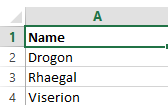
\includegraphics{gfx/dragonNames}} }
\caption{Tabular Data}
\label{fig:tab}
\end{figure}

 When however you consider \autoref{fig:ontoDragons} the meaning of the same data as shown in \autoref{fig:tab} becomes clear; it shows characters from a popular fantasy novel. 

\begin{figure}[!htbp]
\myfloatalign
\fbox{{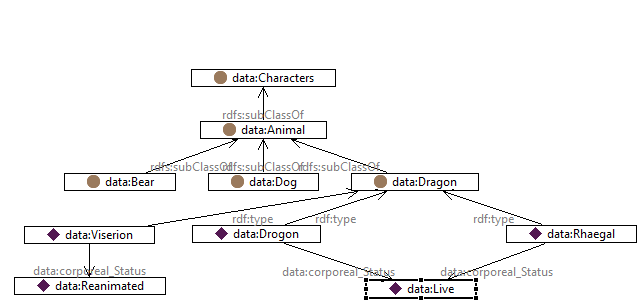
\includegraphics[width=\linewidth]{gfx/gameOfThronesDragons}} }
\caption{Ontology format}
\label{fig:ontoDragons}
\end{figure}

The intention is that by storing the meaning alongside the data it is straightforward, often not even requiring of human intervention, to combine that data with other data stored as information. Whilst this is true of any predefined schema the benefit of this approach is that it does not require such a central standards body to define a schema, instead any stakeholder can create data in this format, extending it to suit their needs, and still be able to integrate it with other data, allowing new data to be represented as and when it becomes available, without a lengthy approval process. 

\subsection{Barriers to adoption}
The fact that ontologies exist, and yet their adoption remains limited, implies that there are barriers to industry adoption of ontology. In the past technological maturity has been a serious obstacle; reasoning over large data stores is computationally expensive and neither robust software optimised for this task, nor hardware capable of running it has been available. Now the requisite hardware is available at a commodity price point and competing vendors for the relevant datastores exist in the marketplace so these barriers are eliminated. However a significant obstacle remains, in the form of a shortage of skilled personnel, ontology specialists and means of handling very high frequency data.

\section{Aims and Objectives}
This thesis will investigate means by which the adoption of ontology by the UK rail industry can be accelerated. It will look at tooling designed to overcome the known barriers to adoption, and how these may be used within a typical industry work-flow. The questions this thesis will investigate are set out in chapter three. 

\section{Thesis organisation}
This document is organised as follows:

\begin{itemize}
	\item Chapter one is this introduction, which aims to set out the main themes of the thesis;
	\item Chapter two provides a review of the available literature on the topics covered by this thesis. In particular, the current situation with regards to data integration in the rail domain is examined, as are successful examples of data integration from other industries;
	\item Chapter three draws conclusions from the current situation out lined in chapter two and gives a more precise definition of the questions this thesis will answer;
	\item Chapter four investigates a typical industry data source and how it can be made available in a linked format;
	\item Chapter five investigates techniques for working with linked data, not requiring of skilled personnel;
	\item Chapter six investigates how multiple data sources can be brought together in an industry context;
	\item Chapter seven draws conclusions as to how data integration can be improved in the UK rail industry.
\end{itemize}

\section{Papers published over the course of this research}

The work presented in this thesis has been presented, in part, at a number of conferences.

\begin{itemize}	
	\item \textsc{Applications of Linked Data in the Rail Domain} \\ \textit{IEEE International Conference on Big Data 2014} \\
	This paper presents early findings from a larger study, into the use of linked data in the rail domain. The study and other literature has shown there to be benefits from improved integration of data in this domain and proposes that linked data in general and ontology in particular will address this. The paper will set out the current state of data integration in the British rail domain, highlighting issues found there. The manner in which linked data is employed in the broader transport domain will then be examined along with previous work pertaining to the rail domain. 
    \item \textsc{Ontology in the Rail Domain} \\ \textit{Knowledge Engineering and Ontology Development 2015} \\
    This paper presents the railway core ontologies, a group of related ontologies designed to model the rail domain in detail. The purpose of these ontologies is to enable improved data integration in the rail domain, which will deliver business benefits in the form of improved customer perceptions and more efficient use of the rail network. The modularity of the ontologies allows for both detailed modelling of the domain at a high level and the storing of instance data at lower levels. It concludes that the benefits of improved rail data integration are best realised through the use of the railway core ontologies.   
    \item \textsc{FROM DATA TO INFORMATION: PROVISION OF RAILWAY DATA TO PASSENGERS IN THE INFORMATION AGE} \\ \textit{World Congress of Rail Research 2016} \\
    This paper puts forward the case for using RaCoOn for data integration in the the rail domain and sets out tools for expanding RaCoOn
\end{itemize}
%************************************************
\chapter{Literature Review}\label{ch:litreview}
%************************************************
This literature review will first summarise the current state of the art in data integration within the rail domain, before moving on to discuss the costs and benefits of greater integration. Linked data and ontology will be introduced as a means of achieving improved integration between data resources, and cases studies from other industries, which have adopted ontology for integration will be examined and conclusions drawn. The discussion will conclude with a summary of how the lessons learnt may be applied to GB rail.
% Lastly a number of techniques used throughout this thesis will be explained.

In the last twenty years the world outside of the rail industry has changed significantly, with information communication technology becoming all pervasive, however the rail industry has been slower to adapt. Although customer information is now commonly provided electronically and commodity software platforms provide multimodal journey planning, these services are only as good as the data fed to them. Within the industry however ICT systems remain siloed, with advances made in the gathering of data but exploitation being limited by system boundaries and commercial barriers. 

\section{State of the Industry}
\label{state}

The Mc Nulty report, a study into value for money offered by GBRail, \citep{DepartmentforTransport2011}, found that:
\begin{quote}
    The effectiveness of the industry’s IS is inhibited by a suite of legacy systems that are expensive to run, unable to communicate with new technology and encourage users to develop a wide range of bespoke local systems to overcome limitations. Many legacy systems were created and managed in company silos, with only a few systems crossing industry boundaries.
\end{quote}

The report goes on to conclude: ``Information systems are at the heart of a more efficient railway that delivers value for money. Allowing the railway’s existing IS to continue unreconstructed will increase cost, reduce efficiency and undermine customer service. In contrast, the replacement of legacy systems and the exploitation of new technology will generate improved value for money.''. Also proposed in the that report was the creation of the Rail Delivery Group, an industry body representing infrastructure, freight, and passenger operators\footnote{Further information may be found at: \url{http://orr.gov.uk/about-orr/who-we-work-with/industry-organisations/rail-delivery-group}}. Another report, created as a response to the The Rail Technical Strategy \citep{TechnicalStrategyLeadershipGroup2012b}, identifies a need for better data integration, stating that:

\begin{quote}
Over 130 information systems maintained by approximately 20 suppliers were in operation in 2011. Maintaining individual legacy systems is expensive and inefficient. Information cannot be shared or exploited efficiently and this inhibits whole-system approaches for technology-based improvements. 
\end{quote}

The \citet{RDG2017} proposes in the \say{Capability Delivery Plan} that: \say{Standards will allow information to be interpreted and combined more easily delivering new insights and intelligence to the industry.}. At the present time this goal is still outstanding. 

The issue of lock in to proprietary systems and the creation of data silos is examined in \citet{Joh13}, which states that
\begin{quote}
    Where electronic data exchange standards for rail do exist, many are proprietary binary formats used to provide point-to-point interfaces between specific systems and not intended for use in a generalised context.
\end{quote}
\citet{Verstichel2011a} finds a need for improved data integration in the larger European rail domain: ``Industry-wide integration in the information domain is only in its infancy. From an efficiency point of view, this field leaves much room for improvement (as did the integration in the mechanical and electrical domain). ''

 \citet{Morris2014} discusses the rising rail ridership in the UK, along with the need for improved efficiency. This trend continues as shown by the official statistics from the Office of Road and Rail, \citet{OfficeofRoad&Rail2016}, with 1.7 billion journeys having been made in the financial year 2016-17, up 0.8\% from the previous financial year; this marks the highest ever number of journeys on the UK rail network, since statistics started being collected in 1950. However it should be noted that this is also the smallest year on year increase since 2009-10.

Since the benefits of improved data integration have been identified, Network Rail the UK infrastructure operator, has taken steps to improve data integration using conventional means. A good example of this is the Linear Asset Decision Support solution, internally referred to as LADS\footnote{technically, LADS is an implementation by Capgemini of Bently Optram}, which brings together fourteen asset information systems, including the Rail Defect Management System, as part of the Offering Rail Better Information Services (ORBIS) program. This system has two front-ends; a hand-held system which can be used on ruggedized tablets track side to access information about nearby assets, and a desktop version for planning purposes. The system can show amongst other things:
\begin{itemize}
    \item Video (or stills) of the track, taken from New Measurement Train;
    \item Track Geometry measurements, also from the New Measurement Train;
    \item Track defect data and reports;
    \item Asset Locations;
    \item Asset type and age;
    \item Maintenance history.  
\end{itemize} 
These datasets are shown together in a ``swim lane'' view. This proprietary system covers the asset maintenance domain and will need extensive development to add new data sources or outputs. 
 
The amount of data used within the rail domain has increased rapidly with time. As it has become possible to collect more data on asset condition the volumes of data relating to each asset have grown, for example the work done in response to the \say{FuTRO Universal Data Challenge} reported by \citet{Tutcher2015a} suggests that large volumes of data\footnote{up to\say{15 seconds of data, sampled at 4kHz, for eight sensors}, though this can be down-sampled.} would need to be recorded every time a sets of points moved, anywhere on the rail network. Techniques such as alternating current field measurement sensor (ACFM) as discussed by \citet{Rowshandel2013} also produce large volumes of data, in this case relating to rail condition. Others sources of high volumes of data include ground penetrating radar, to assess trackbed condition, as reported by \citet{eriksen2004improved}. An assessment of the growing volume of data in the rail domain in an American context was performed by \citet{Zarembski}, which finds condition monitoring to be a likely source of growth. The European rail network is considered in \citet{Nunez2014}, which also studies data used for maintenance in the rail domain, taking as a case study the Dutch Rail Network. In the UK large volumes of  data are collected by the New Measurement Train and significant value could be added to this if it were easier to match readings with the assets to which they pertained.

The current work flow with regards wheel impact load detection is an example of less successful integration, which was described by \citet{Tutcher2015} as  ``several interfaces between machine and human operator railway data management exist as wheel impact data is taken from its silo, manually compared to train running information in another silo, and finally input into a maintenance system silo''. Wheel impact load is important because it detects when train wheels are damaged, thus in turn causing damage to the track and train alongside causing discomfort to passengers.

\subsection{Information Security}

Alongside the growth in data stored electronically comes a second, related, issue; that of IT security. As data has become more distributed and greater use is made of the public internet further precautions are required. The importance of this in the rail domain is discussed by \citet{Depar2016}, and further discussions in the context of the cybersecurity of signalling systems may be found in \citep{BloomField2016} and \citep{Chen2015}. In \citet{Chen2015} the security of passenger information systems is also considered.

\section{Ontology}\label{onto}
In \autoref{ch:intro} of this document ontology was defined as: 
\begin{quote}
\emph{an explicit specification of a conceptualization}
\end{quote}
The author of that quote, Tom Gruber, has gone on to provide a more complete definition in \citep{Gru09}. 

\begin{quote}
\begin{itemize}
\item An ontology defines (specifies) the concepts, relationships, and other distinctions that are relevant for modelling a domain.
\item The specification takes the form of the definitions of representational vocabulary (classes, relations, and so forth), which provide meanings for the vocabulary and formal constraints on its coherent use
\end{itemize}
\end{quote}

Data integration was one of the first benefits of ontology to be identified, as early as 1991 and was already under discussion \citep{Siegel1991}, along with several other uses cases that remain relevant today. \citet{Siegel1991} aimed to enabled the \say{integration of multiple disparate database systems} by using a ``common metadata vocabulary'' and suggested that \say{global ontology to provide the common vocabulary and all component systems must provide semantic mappings to that global ontology}. This approach remains broadly valid today, though the available implementation toolsets have improved significantly. 

An ontology could be described a means of storing a view of the world, in this context, it stores information, not simply data. Beyond that ontologies allow reasoning to be performed and new information to be inferred from the facts and rules it contains. This can be used simply to categorise objects, itself a powerful mechanism \eg things may be classified as faulty or working, according to their properties. Rules can however be used to abstract other logic; would it be wise to offer insurance based on the provided circumstances for example. Reasoning allows strict mathematical logic to produce results, for example: \(\forall L \exists D \cap T \) where L is life, D is Death and T is taxes represents the proverb: \say{In this world nothing can be said to be certain, except death and taxes}. The development of ontologies from First Order Logic is covered in depth in by \citet{baader_calvanese_mcguinness_nardi_patel-schneider_2007}.

\subsection{Ontology Reasoning}
In the context of computational ontology, reasoning is used to imply facts not originally known or stored based on existing facts in the triple store. For example, if you know that every human has exactly one biological mother who is female and one father who is male, persons F and M are C's parents, and that person M is male, you may infer that person F is female.  This is discussed in depth in section 2.4.5 of \citet{Tutcher2015}. Reasoning can also be used to ascertain whether the concepts from two different models represent the same thing, or for classification of objects against a hierarchy within the ontology model. This has been used for purposes as diverse as ascertaining the correct pension to pay someone, based on their employment history, through to assigning biological systems to groups. In the rail context it has been used in multiple projects to ascertain if a combination of circumstances implies a fault.

\subsection{Ontology related terminology}

When discussing ontology the thesis will use the following terminology:

\subsubsection{Triples}\label{sec:trip}
When ontologies are stored electronically they take the form of triples, a statement broken into three parts, the subject, the predicate and the object as illustrated in \autoref{fig:joffrey}. Anything refereed to by a triple should have a unique identifier, known in this context as a Uniform Resource Identifier or URI. The W3C recommends that these URI's take the form of Uniform Resource Locators commonly abbreviated URL and that further more these Uniform Resource Locators point to a resolvable domain name. Whilst this is considered best practice it is entirely possible to create an ontology were the URIs are not URLs. Each part of a triple can be a URI itself, however, it is also possible for the object of a triple to be a simple value or a ``blank node'', that is a node with no name, used to link to further nodes.
\begin{figure}[hb]
    \myfloatalign
    {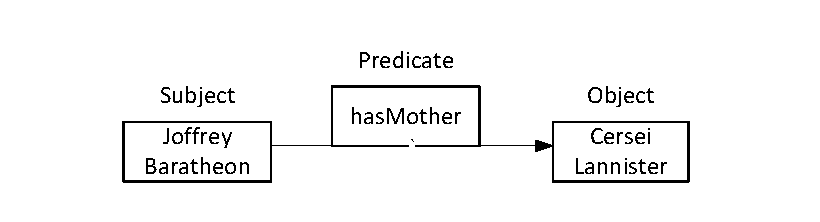
\includegraphics[width=\linewidth,keepaspectratio]{gfx/JofferyTriple}} 
    \caption[Triple]{The parts of a triple. Note that the content of each box is commonly a URI}
    \label{fig:joffrey}
\end{figure}
In this context a triple can also be thought of as a directed graph, in which the Subject and Object are both nodes.

\subsubsection{Tbox and ABox}
Throughout this discussion the terms ``TBox'' and ``ABox'' will be used. The TBox or ``Terminology'' box refers to that part of the ontology that holds the definitions and concepts. The statement ``Humans are a type of animal'' would generally belong in the TBox of an ontology. The ABox or assertion box holds assertions made using that knowledge, one such assertion could be \say{Chris Morris is a human}. In a relational database terms TBoxes and ABoxes are comparable to the schema (TBox) and the data (ABox).

\subsubsection{Expressivity}
Ontology expressivity is the complexity of the concepts that can be represented in a given form. Expressivity is generally described using Description Logic (refereed to in the literature as a DL), which are in turn decidable fragments of First-Order Logic. Different DLs represent different sub-sets of First-Order Logic and are annotated according to how expensive they are. 
\citet{Horridge2012} discusses some common levels of expressivity, in section 2 of the paper:
\begin{itemize}
    \item  \(\mathcal{AL}\) Is amongst the most limited, supporting:
        \begin{itemize}
            \item   Intersection  \(\cap\);
            \item   Universal quantification (All Value From) \( \forall \);
            \item   Limited existential quantification, with restrictions \( \exists\) ;
            \item   Atomic Negation \(\neg \) .
        \end{itemize}        
        The limitations of \(\mathcal{AL}\) description logic restrict the complexity of the concepts that can be encoded and, as such this DL is not commonly used, aside from as a basis for more complete description logics.
        \item With Full Negation this becomes  \(\mathcal{ALC}\). This means that any concept, not just atomic concepts (generally variables in first order logic), can be negated. Certain approaches, such as that discussed by \citet{Meyer2006} limit themselves to the \(\mathcal{ALC}\) description logic, since most operations can be performed on it in polynomial time.
        \item Adding hierarchy - sub-properties makes this \(\mathcal{ALCH}\)
        \item Adding nominals (only one can exist), inverse properties (lifts is the inverse of liftedBy for example) and numerical restrictions gives - \(\mathcal{ALCHOIN}\). 
        \item Add transitive properties, for example \say{if x is a part of y and y is a part z then x is a part of z} gives \(\mathcal{SHOIN}\), because \(\mathcal{ALC}\) with transitive properties is abbreviated \(\mathcal{S}\). As discussed by \citet{Horrocks2006a} \(\mathcal{SHOIN}\) underpins OWL 1 and thus is very widely used.  
\end{itemize}
More expressive DLs exist, but increasing the complexity of the concepts expressed also increases the complexity (and thus computational time required) of reasoning. A more expressive DL still, \(\mathcal{SROIQ}\), is used as the basis of the OWL 2 (discussed in \autoref{sec:standards}). This DL allows for properties to be disjoint,reflexive, irreflexive or antisymmetric as well as all the properties found in \(\mathcal{SHOIN}\). For a description of \(\mathcal{SROIQ}\) see \citet{Horridge2012} section 2 or for greater depth: \citet{Horrocks2006}. A tool for the comparison of various description logics may be found at: \url{http://www.cs.man.ac.uk/~ezolin/dl/}.

Choice of level of expressivity is very important in ontology design and is considered in depth by \citet{Tutcher2015}. In that work the danger of allowing too much expressivity and making it either difficult or impossible to use automated tools to carry out reasoning is discussed. Since it is expected that reasoning will be used over ontologies in this the rail domain, the question of expressivity will be further considered in the remainder of this thesis.

\subsubsection{Upper Ontologies}
When technology first made it possible to store logic and ontologies electronically and to perform reasoning computationally many studies proposed upper ontologies. That is ontologies that, in keeping with the philosophical basis of the term, aimed to be \say{Theories of everything}, to hold all of humanities knowledge. This resulted in several projects; foremost amongst the early studies was SUMO, the suggested upper merged ontology, proposed by \cite{Niles2001}. Latterly a number of other upper ontologies have emerged, such as  BFO or basic formal ontology, which is considered in the context of the biomedical domain by \citet{Grenon2004}. The advantage of using a common upper ontology is improved integration \emph{between different ontologies}. It can be seen that whilst this idea is much discussed in the literature examples of it's practical implementation are harder to find.

\section{Standards for data integration}\label{sec:standards}
One domain in which significant progress has been made is that of standards for interoperability of ontologies and the formats in which they are stored.

\subsection{Basic Standards}
There are several low level standards upon which the other standards this document will consider are built.

\subsubsection{XML}
Several current standards in use within the industry are based upon Extensible Mark-up Language (XML). XML is defined by \citet{W3.org2013} as \say{application profile or restricted form of SGML, the Standard Generalized Markup Language [ISO 8879]}. Standard Generalized Markup Language (SGML) is in turn a means of specify a document structure, of which HTML (Hyper Text Markup Language) is the best known. XML is a data description language which uses SGML, effectively it is a way of specifying a data transfer. It is comparatively verbose and can, though does not have to be, designed such that it is human readable.  

\subsubsection{Resource Description Framework}
The Resource Description Framework, here on referred to as RDF, is a standard that can be used for the interchange of linked data and ontologies. Defined at by the W3C a guide is available in \citet{Wood14}. RDF is was initially used primarily for the provision of metadata from conventional websites and is still commonly used within the semantic web. RDF forms the basis for other standards, most notably Web Ontology Language \autoref{sec:OWL}. It should be noted that while it is quite possible to use RDF triples out of an ontology driven environment, RDF alone does not provide sufficient contextual information to enable reasoning operations to take place.

\subsubsection{Web Ontology Language}\label{sec:OWL}
OWL or Web Ontology Language has become the standard for ontologies which are to be shared online. OWL is a recommendation from the W3C, the de facto standards body for web standards. Other domain specific languages have been developed in the past, sometimes with greater expressivity than OWL, however these have not seen wide adoption. The OWL 2 was released in 2012.

The OWL guidance document by \citet{McGuinness04} explores the comparison between XML and OWL, specifically it poses the question ``What does this buy me that XML and XML Schema don\'t?'' and suggests firstly that OWL (and this point applies equally ontologies in general) provides a form of knowledge representation, not just a schema. From a schema you know how to respond to an expected message, but nothing else is possible. Secondly the same document also states that once a reasoner has been constructed it can be applied to many domain ontologies, thus promoting reuse.

The specification for OWL 2 may be found at in \cite{Parsia:09:OWO} and a guide in \citet{Parsia12}. OWL 2 became available during the development of the RaCoOn ontologies and has the following ``Profiles'' available, the details of which are considered by \citet{Parsia12}:

\begin{itemize}
    \item OWL 2 Full Consistency checking and entailment checking are undecipherable at this level, however this offers the maximum possible expressivity of any profile. 
    \item OWL 2 EL This uses a DL called \(\mathcal{EL}^{++}\) - discussed in \citet{Baader2005} \(\mathcal{EL}^{++}\) is a good comprise of tractability and expressivity in particular because it can be reasoned over in polynomial time, whilst still capturing the complexity of large ontologies. This profile was designed with the biomedical domain in mind, where it is used extensively, since ontolgoies in this domain often have complex T-Boxs and very large A-Boxes;
    \item OWL 2 QL As stated in \citep{Parsia12} this DL \say{can be realized using standard relational database technology}. The intended use case of this profile is to build on the years of development and optimisation around classic relational databases, by implementing Ontologies that leverage these systems as their datastores;
    \item OWL 2 RL is more restrictive than the previous two profiles, aimed at working with RDF data at scale, giving fast reasoning over large datasets;
    \item OWL DL ``Direct Semantics'' is the subset of OWL 2 which is required to implement \(\mathcal{SROIQ}\). This is larger than any of the other profiles listed above, but is still only a subset of OWL 2 Full. Ontologies complying with the DL sub-language of OWL (as opposed to OWL 2) are automatically valid OWL 2 DL ontologies, which is useful for backward compatibility. 
\end{itemize}

\subsubsection{SPARQL}
\label{sec:lit_rv_sparql}
SPARQL, a recursive acronym meaning ``SPARQL Protocol and RDF Query Language'', is to query ontology data-stores and to perform  \say{Create, Read, Update and Delete} or CRUD operations, an overview is provided by the \citet{5403219}. Syntactically and functionally SPARQL bears comparison to SQL, the Structured Query Language used with relational databases. Both facilitate CRUD operations including very complex criteria for selection, however SPARQL differs in that the the data to be queried will always be RDF triples. SPARQL offers complex filtering and selection functionality alongside 

\subsubsection{GEO SPARQL}
Geo-SPARQL is an extension of SPARQL, as discussed in \autoref{sec:lit_rv_sparql} for handling geographic data. It is defined by the Open Geospatial Consortium\footnote{The definition is available from \url{http://www.opengis.net/doc/IS/geosparql/1.0}} in \citet{Perry2012}. This makes it possible to ascertain if a given point is within an area, if two area's intersect or to find the distance between two points, for example. It can use a number of different coordinate systems and convert between them. It is used, in conjunction with SPARQL, to write more complex queries which can take into account an items location.

\section{Software tools}
The commercial market for ontology related software has grown significantly in recent years and there is now a selection of tools available for many different ontology operations. Ontology editing tools, reasoners and triple stores are all competitive market places, with both commercial and open source products available in all spheres. Another area in which a range of tools is available is that of moving from relational database to ontology and linked data. If the database schema is taken as the T-Box and the row data the A-Box, then it is possible to design an automated tool to do exactly this and make the data available as an ontology. A method for recording the mappings of relational databases to ontologies is discussed by \citet{Dimou2014}, and a survey of the available tools for automating the process is available in: \citep{Spanos2012}. As discussed throughout the literature, a fully automated approach often produces a slightly idiosyncratic T-Box and better results may be achieved by running a first automated pass then a human intervention to improve the model.

Many software tools were required for project. Some such as the integrated development environment, were selected purely on the grounds of experience; familiarity with a tool is very valuable on it's own, thus visual studio\footnote{details of this product and the various editions available are available from \url{https://www.visualstudio.com/}} and C\# were used for the majority of the software development. Another tool required was an ontology editor for the making additions and alterations to the rail core ontologies. Many such tools exist and \citet{Erlingsson2016} provides a review of the most popular. Top Braid composer Maestro Edition \footnote{Available from \url{https://www.topquadrant.com/tools/modeling-topbraid-composer-standard-edition/}} was selected for this project owing to the comparative speed with which it was possible to add large numbers of individuals along side the useful visualisation functionality. 

In order as to store data in a linked format it is necessary to use a triple store. A triple store is a data store which holds information in as triples, as discussed in \autoref{sec:trip}. All triple common triple stores provide basic CRUD functionality, however they can be differentiated on a number of grounds: 

\begin{itemize}    
    \item Cost and License. Some are open source, others offer free trails or reduced academic license others are commercial products, commonly have significant licensing costs;
    \item Performance. How rapidly operations can be performed on given hardware and thus what the minimum hardware required to achieve reasonable performance. This includes not just CRUD operations but also to reasoning over the ontology;
    \item Security. Many triple stores offer some form of access control, with varying levels of granularity. Some triple stores support access control per graph, some allow for multiple datastores to be hosted by the same server with different permissions and access control lists. Triple stores can also have groups and roles, similar to traditional relational databases, to allow bulk management of user access;
    \item Extent of available support. Triple stores range from abandoned academic projects to commercial offerings with support contracts;
    \item Compatibility. This consideration is key when the other technologies in the system have already been selected.
    \item Extra features. Many triple stores offer features beyond CRUD, not all of which are relevant to all implementations;
\end{itemize}

The market for triple stores has is evolving rapidity at present and a number of new products are emerging, however, due to the existence of previous work on which this thesis was based, Stardog\footnote{Made by Clarke \& Persia, download and further details available from: \url{http://www.stardog.com/}} was selected. This was then accessed on the criteria above:

\begin{description}    
    \item[Cost and License] A \say{community edition} is available for free. Certain projects required features not available in that edition, however and for that an arrangement was made with Clarke \& Persia.
    \item[Performance] No benchmarking was undertaken by this project, however, very large inserts were performed in very satisfactory time frames.
    \item[Security] Stardog offers per graph security. Each database can contain many graphs, if the user desires.
    \item[Support] Extensive documentation is provided, additionally questions are always quickly responded to in the public support group.
    \item[Compatibility] Interfaces exist to use this triple store from both JAVA and C\#. The triple store itself can run operating system for which a Java virtual machine is available.  Additionally scripts had been written to insert data into that triple store.
    \item[Extra features] This has evolved significantly over the duration of the project, however most useful amongst the non-standard features was the web interface for administration. 
\end{description}


\section{Benefits of ontology for data integration}
\label{benefits}
The available literature suggests several related benefits from using ontologies for data integration within the rail domain. In the \say{Capability Delivery Plan} the \citet{RDG2017} consider data integration with a focus on cost reduction and use of data as an enabler of other technologies. \citet{Tutcher2013} discusses this with an emphasise on remote condition monitoring. Another commonly cited beneficiary of ontology enabled data integration is passenger information as reported in  \citet{Verstichel2014}. This work presents the TraPIST project, which implements a framework for data integration using ontologies and creates a real time passenger information application as a demonstration.

The advantages to the rail domain of using ontology are discussed in \citet{Morris} based on discussions with the UK infrastructure manager, Network Rail, as well the study reported in: \say{Factor 20 – reducing CO 2 emissions from inland transport by a major modal shift to rail} by \citet{Roberts2011}. The use cases examined in that study were:
\begin{description}
    \item[Customer Information] Many studies have found benefits to customer information from improved data integration using ontologies. The objective of bringing together multiple data sources is considered by \citet{Verstichel2014}, with the aim of going beyond simply informing the customer of the time table and when a particular train is expected, to outlining possibly connections and routes through the station in light of real time information. This work also took into account the differing levels of mobility offered different passengers have, taking into account disabilities luggage and other similar constraints.
    \item[Predictive maintenance]
    This is an area in which ontology acts as an enabler, making other technologies possible. Many previous studies have addressed the area of predictive maintenance, but it is only possible when data is available, as discussed by \citet{Umiliacchi2011}. The project reported in \citet{Tutcher2015a} also addressed this issue and produced a demonstrator focused on points machine condition monitoring. 
    \item[Train Identification]
    The linking of track-side information with running services is discussed in \citep{Morris}. Condition monitoring of in service vehicles from the track-side currently presents challenges linking the vehicle detected to a physical unit is a problem. 
    \item[Maintenance Timing and Forward Planning]
    Two scenarios put forward by the UK infrastructure manager, Network Rail, and reported by \citet{Morris} concerned \say{forward looking question answering}. An interface should be provided to allow the asking of guided (not truly free text) questions such as: ``Given the data we have when would be the best time to do maintenance?'' or ``Is it better to replace a given asset, such as a bridge, like for like or with a less expensive substitute, such as a bridge rated for a lower weight?''    
\end{description}
    
Several European research projects, most recently IT2Rail as reported by \citet{Gogos2016}, discuss the advantages of using ontology for data integration in the rail domain. As with previous studies, such as InteGRail, reported  by \citet{Kopf2010}, \citet{Gogos2016} find ontology brings benefits to the industry as a whole, although the benefits do not necessarily accrue with the same party as the costs. A key advantage of using ontology for data integration, as espoused in \citep{Gogos2016} and \citep{Morris}, is that of decentralising data entry; because the ontology model can be extended by anyone, there is no limit on who can make data available via local extension, as such suppliers can provide data relating to their own products, reducing the data entry burden on any stakeholder. Furthermore the architecture of semantic web means that there is no need for a central repository of all rail related data, though security restrictions may be placed on who can access certain data when that is necessary.

Several EU funded projects, building on the outputs of IT2Rail, are in progress at the time of writing. The \say{ATTRACkTIVE} project aims to develop a \say{one stop shop} type phone application handling everything from ticket purchasing to routing around disruptions. `Co-Active' has similar goals, but focuses primarily on the distribution of revenue from a single journey across multiple providers. Both these projects aim to work across multiple modes. In general ontology can bring a range of benefits to the customer information domain, integrating data from various sources to provide more comprehensive information. 

Ontology is also being explored commercially, \citet{ERTMSSolutions2017} of Brussels state that they have obtained a contract for the use of their ontology based data integration tools on the Belgium rail network, working for SNCB, the Belgium national rail company.

\subsection{Multi-modal transport}\label{subsec:multi}

Multi-modal transport is a domain in which, almost by definition, there is a need for data interchange; Journeys tend to be multi-modal, and thus it is beneficial for journey planning applications to include data on all modes. The multimodal journey problem was first considered in the ArkTRANS project, as reported in \citep{Natvig2003} and ArkTRANS has become the basis of a number of projects concerned with the integration of data for freight.Examples include: \citet{Gonczy2012} , \citep{Rodseth2011} and \citep{Paganelli2009}. Multimodal in the case of freight often includes an element of the journey made by sea freight which is considered by \citet{Rodseth2011} or by ferry.

Work reported in \citet{Verstichel2014} includes a customer assistance application, which aimed to give personalised customer information for users making multi-modal journeys. Using data from multiple sources, both timetable and actual running, along with GPS position and personalisation setting, such as the user mobility the application will attempt to suggest the best modes of transport to complete a journey, according to the users selected metric (cost or time). 

\citet{Morris2016} discusses Google Transit Feed Specification, here on refereed to as GTFS. GTFS is a format, initially defined by Google, is a format for the interchange of public transportation schedules. This primarily used for journey planning, both by Google maps and other third party applications, both open and closed source.  GTFS is discussed by \citet{Santos2014} and it's success should be noted; much public transport information is now available to google maps. Possible improvements to the protocol are discussed in \citet{Santos2014} and further improvements have been proposed by google, in particular to allow real time information to be added to the map, regarding departures and service status. The original GTFS defined at: \url{https://developers.google.com/transit/}. It can be seen that GTFS is a fairly simple relational format. It is heavily used, as described by \citet{Colpaert} ``The General Transit Feed Specification (GTFS) specifies the headers of 13 types of CSV [Comma Separated Variable] files, describing the schedules using a set of rules. In recent years, GTFS gained a lot of popularity, thanks to its simplicity and its adoption in popular route planning systems such as Open Trip Planner, Navita.io, Google Maps or RRRR Rapid Real-time Routing.'' The work in \citet{Colpaert} uses GTFS and linked data fragments to perform multi-modal route planning. It should be noted that GTFS was originally ``Google Transit Feed Specification'' however it became an open source project, no longer funded by Google. GTFS real-time can be used transmit perturbation information, allowing for journey planning software to update plans as services alter. 


\section{Data integration in other industries}
Many other industries are far ahead of the rail industry in terms of take up of ontology. \citet{Morris2014} discuss, and draw lessons pertinent to the rail domain from applications of ontology in, the biomedical research, media, petrochemical, and power distribution domains. This is further discussed by \citet{Horrocks2007}, who which mentions applications in the following industries: eScience, geography, engineering, medicine, biology and defence.

\subsection{Industries implementing Ontology}
\subsubsection{Biomedical Research and Bioinformatics}
\label{sec:biomedical}
The Biomedical domain remains at the forefront of ontology development and uptake.

As early as 2004 the Gene Ontology (GO) was available for use, and was described as by \citet{Smith2004} as comprising: \say{1395 component terms, 7291 function terms, and 8479 process terms.} The purpose of this ontology is described as: \say{to allow researchers annotating genes and gene products to locate where the features and attributes they are addressing in their work might lie (their position in logical space) in relation to other, more familiar features and attributes and thus either to pick out corresponding terms already existing within GO’s controlled vocabulary or to localize corresponding gaps in the existing hierarchies and so recommend new terms which need to be included.}.  In 2006 \citet{Bodenreider2006} summarised the the role of ontologies within bioinformatics as as having ``moved from a niche activity to one that is, in all respects, a mainstream activity''. That study includes a time line, until 2006 (when it was published) of use of ontology within bioinformatics, which shows a move from ontologies designed by computer scientists to ontologies produced within the bioinformatics community. Focusing specifically on the Gene Ontology, \citet{Bodenreider2006} state that it grew from 3500 terms in 1998 to 20,000 terms in 2006. It is worth noting that both \citet{Bodenreider2006} and \citet{Gro2016} as with other studies in the domain of bioinformatics are careful to state that they are defining ontology quite broadly; there is room for argument, though it is beyond the scope of this thesis, as to whether some of the ontologies in this domain might more properly be termed ``controlled vocabularies''.

A recent study, by \citet{Gro2016}, focuses on mapping the various related ontologies in the bioinformatics domain together and studying how they change. It finds 500 different ontologies to be in use at this time in bioinformatics. These largely cover different sub-domains, though there is some overlap. This high uptake of ontology has been encouraged by requirements, imposed by some journals in this domain, that results be published annotated with an approved ontology. This is intended to make data available for automated processing and unambiguously.

SNOMED CT is another ontology in the Biomedical domain with a long history, created as merger of two standard vocabularies, both of which pre-date storing ontologies electronically. As \citet{Chute2000} states in his comprehensive review of the history of SNOMED CT, the precursor to SNOMED CT was \say{Conceived during a symposium at the New York Academy of Medicine in 1929}, well before ontologies were considered for data representation. The same author goes on to discuss the breakthrough represented at the time by accurately coding clinical conditions so as to remove ambiguity. This evolved through time first as taxonomy, storing electronically both very detailed and high level terms, along with how they such terms can be related, to its present light weight and well regarded ontology.  Based on a light weight decision logic, \(\mathcal{EL}^{++}\), this ontology consistently reviewed by academics and whilst scope for improvements is often found it's utility is unquestioned. 

\citet{Jovanovic2017}, whilst primarily focused on the semantic annotated of existing textual biomedical papers, also contains a review of the current (as of 2017) state of ontology within the biomedical domain.

\subsubsection{Media}
\label{sec:media}
The British Broadcasting Corporation, here on referred to as the BBC make extensive use of ontology, both internally and externally\footnote{A promotional video  for the BBC's work in this area may be found at: \url{http://www.bbc.co.uk/academy/technology/software-engineering/semantic-web/article/art20130724121658626}}. The BBC adopted linked data technology at a comparatively early stage; \citet{Geo09} discusses the BBCs aspirations and future plans in this area along with summarising progress to date and says: ``we demonstrated how these links between data items can benefit our user facing web sites, through topic pages and navigation badges.''. The BBC makes use of several external data-stores, most notable amongst them DBPedia - \url{http://wiki.dbpedia.org/}, a linked data companion to Wikipedia. This approach, of reusing available data sources rather than recreating them is recommended through out the literature. At the time of writing DBPedia contained  entries for 5.2 Million entities \footnote{\url{http://wiki.dbpedia.org/dbpedia-version-2016-04}}, encoded using nine and a half billion RDF triples. DBPedia has similar coverage to Wikipedia, that is to say, some information on almost all topics, but to a limited depth. The rail-domain is covered, for example a class 700 electric multiple unit (as used in the Thames Link program) is described at \url{http://dbpedia.org/resource/British_Rail_Class_700}.

As discussed by \citet{Mikroyannidi2016} the BBC have continued to make progress in this area, now covering the education domain.  
\subsubsection{Process and petrochemical plant}
 ISO15926 was published in 2004, having originally been a standard for exchanging technical drawings, used in a range of manufacturing sectors, including defence. A history of ISO15962 is available from: \citep{POSCCaesarAssociation2011}. ISO15926 has been used extensively by oil companies working on the ``Norwegian Continental Shelf''. As discussed by \citet{Leal2005} key components of the standard are a reference data model and an information model. The concepts used in ISO15926, and in particular it's approach to modelling changes over time, were important in informing the design of the rail core ontologies, as discussed by \citet{Tutcher2015}, along with a more detailed break done of the standards components. 
\subsubsection{Power Distribution}
The common information model, as used in the power distribution industry, is extended by \citet{Hargreaves2013} to include use of ontology for information exchange. This common information model is also used as an enabler of ``smart grids'' as discussed by \citet{Fremont}.

\subsection{Other Domains}
There is early stage work on going work in several domains, at various levels of maturity, beyond that reported in \citep{Morris2014}.

 \subsubsection{Manufacturing}
\citet{Mueller2015} propose use of ontology as a means to reduce energy consumption in the manufacturing sector. Many factories use equipment from a range of suppliers integrating data about the equipment can produce a number of benefits this work focuses on allowing temporarily unused equipment to enter a low power or ``standby'' state. Different equipment has different prerequisites for this and requires different control signals so to do. A generic manufacturing ontology was also produced by \citet{Mazzola2016} called \say{CDM-Core} developed within the European research project, CREMA.
\subsubsection{Geospatial}
The geospatial domain is another strong candidate for data integration. There are many heterogeneous data sources and a large range of consumers. Example sources cited by \citet{Zhang2013} are `Wikimapia' and Open Street Map, which provides ``elevation and address information, such as state and county name, in addition to the building names, longitudes, latitudes and polygons'' where as  ``Wikimapia provides names, latitudes, longitudes and polygon outlines for building entities'' The same source goes on to note that where details are provided for the same field they do not always have the same value. 

In \citet{Zhang2013} a technique is presented, using a combination of spatial and semantic data integration to combine multiple data sources and present them to a user. This domain is of particular relevance because it exhibits strong cross over with the rail domain since many problems in the rail domain, including those encountered in this thesis, involve locations. The location both of fixed infrastructure and of rail vehicles is of particular interest and certainly overlaps the geospatial domain. An example is given in \citet{Janowicz2012} of two weather stations which both provide wind direction data, semantic disambiguation of blows from and blows to (given as numbers between 0-360) would be useful. \citet{Janowicz2012} Also states that there have been a number of useful ontologies developed in that domain; both mapping ontologies including those from state mapping organisations and domain ontologies such as SWEET, for earth and environmental science. The sensor data integration that is done in this domain is equally relevant to the Rail Domain.
\subsubsection{Finance}
The finance domain has also used ontology for data integration, however, whilst the \say{Financial Industry Business Ontology} allows for interchange of information between companies. In \citet{Kim2004} this is discussed in a Korean context.
\subsection{Virtual Personal Assistants}
Siri, the ubiquitous virtual personal assistant found on most Apple branded devices, was developed by Tom Gruber (who's definition of ontology is quoted in the introduction). This tool uses ontology not just to look up the answers to questions it is asked but ascertain context; it using ontology to store information. This is presented by \citet{Gruber2009}.

\section{Progress towards improved data integration in the rail domain}

\subsection{Non-ontology data integration}
Data integration has been required within the rail domain since before the data was held electronically. Standards were developed for data interchange on an as required basis, whenever two or more systems to communicate. Many of these have evolved over time and have value in different domains. The key weakness with all such approaches is their inflexibility; when the information to be exchanged changes so must the standard, such interfaces are however generally computationally inexpensive to implement. 

Without some standardisation cross border rail travel would be impossible, first vehicles must be compatible in all regards with the infrastructure up which they run, from the gauge of the wheels, through to the in-cab signalling systems. Secondly timetabling information, trains movements, and signalling data must all be exchanged so that the train arrives where it is expected and fits in with local traffic. Lastly financial data needs to be exchanged; usage fees paid for lines travelled upon and electricity used, passenger fares split between operators.


An assessment of the common data interchange standards currently in use may be found in Chapter 3 of \citet{Tutcher2015}, which discusses their application within the following systems and interfaces for GB rail:
\begin{description}
    \item[DARWIN] is the current UK solution for providing real time passenger information, bringing together train describer information with information from various operating company specific systems which offer better precision. This is then made available both to station displays and to external users via web-services.
    \item[ORBIS] Offering Rail Better Information Services (ORBIS) is described in \citet{Tutcher2015}  as \say{a series of projects centred around providing staff with better access to existing asset information data}, before going on to conclude: 
    \begin{quote}
       [ORBIS] coordinate[s] with efforts across the European Union to develop standardised railway infrastructure models. Whilst the data acquisition and design of many of these systems is already under-way, the company recognises that semantic data models provide a longer term solution to ensuring that information is available across the entire organisation.
    \end{quote}
    Amongst the outcomes of this project are LADS, as discussed in \autoref{state}, and a \say{Close Call} reporting application to improve safety, as discussed by \citet{Rail}.
    \item[railML] development of this standard commenced in 2001. Some of the development of the RaCoOn ontologies was based upon terms extracted from this XML standard for data interchange within the rail domain,  in particular the modular structure, with time tabling, rolling stock, and infrastructure is copied from this and as discussed in \citet{Tutcher2015}. Further more as stated in \citet{Tutcher2015} railML is used as ``a data source for railway vocabulary and concepts'', in keeping with the principle of re-use, not redevelopment. RailML uses XML to define its schema. As of version three railML now uses RailTopoModel\footnote{More information available from \url{http://www.railtopomodel.org/index.php/en/}}, codified by the Internal Union of Railways\footnote{Known as the UIC, further information is available at: \url{http://uic.org} } as International Railway Standard(IRS) 30100, as its data model (for infrastructure data). This data-model is itself a graph, and would very naturally lend it self to implementation as an ontology. This is further discussed by \citet{Nash2010}.
    \item[Technical Specifications for Interoperability] Telematic Application for Passengers and Freight service, commonly referred to a TAP (Passengers) and TAF (Freight). Technical standards for interoperability are mandated by the European Union in directive 2008/57/EC - \citet{CounciloftheEuropeanUnionq2008}. These standards set out requirements as to the type of information that must be available to passengers and freight operators, as well as providing a detailed technical standard setting out how this data shall be exchanged. This standard, as with railML, make heavy use of XML for data interchange.  
\end{description}

Another area in which integration is necessary is that of signalling and train control. It is desirable that, when a train crosses a national border it is not necessary to change the locomotive for one compatible with the new nations signalling systems. Similarly journey times can be reduced if it is not necessary to change driver, for one familiar with local signalling conventions, every time a border is crossed. The European Railway Traffic Management System, which is a project overseen by the European commission, aims to make this possible for member states.

\subsubsection{European Train Control System}
\label{sec:etcs}
The European Train Control System, commonly refereed to as ETCS, is intended as replacement for traditional rail signalling systems and forms a part of the The European Railway Traffic Management System (ERTMS). This system provides a standard in-cab element, known as the Driver Machine Interface (DMI) which provides the driver with a range of crucial information, such as whether it is safe to proceed and the maximum safe speed. 

ETCS can be implemented to different levels, with higher levels allowing for a greater density of traffic on the rail network, but requiring of greater investment to implement. The lowest levels ETCS works with pre-existing national signalling systems to provide unified driver information, communicating with line-side equipment via balises. At higher levels the communication uses a radio link. When implemented fully and to it's highest level, three, it uses accurate knowledge of the location of each train on the network to run trains closer together than conventional signalling systems allow for. The full details of this system and it's advantages are beyond the scope of this thesis but are summarised by \citet{EC2011}.


\subsection{Ontology based integration within the rail domain}
\label{sec:prevonto}
Previous work has been done constructing ontological models of the rail domain.

The REWERSE project reported in \citet{Lorenz2005a}, part of the Sixth Framework Program, produced an ontology which covered the transport domain. The purpose of this project was primarily to enable the interchange of geographic information, thus transport modes are covered in some depth, including interchanges between modes and routes taken. Further to this the REWERSE ontology allows for the modelling of timetables for all modes of transport, along with restrictions such as speed, class of vehicle etc. Whilst the goal of this project was not to provide an ontology suitable for detailed evaluation of vehicles or fixed assets within the rail domain it could be applied to the integration of multi-modal transport.

The InteGRail project reported in \citet{Kopf2010} was a European project also funded as part of the Sixth Framework Programme. This aimed to produce both an architecture and an ontology for data integration, to act as a standard for data interchange within Europe. This project produced a \say{network statement checker}, this tool allowed users to check if a given train consist was compatible with a chosen route, by means of demonstrating the capabilities of ontology for data integration. The work done as part of InteGRail is discussed further in \citet{Verstichel2011}, as is the importance of adding semantics to data for improved integration. 

The InteGRail project made it possible to integrate data originating but not only from different manufacturers but also different countries. There are significant challenges to running trains across national boarders, where the information systems relating to the rail network are implemented nationally. At the simplest level it is simple to ascertain whether a track is of the same width, or gauge, as that required by the proposed train consist. Other details are more challenging; the required characteristics of the electrical supply in terms of voltage, frequency, and current must be correct, as must the means of ``picking up'' the power be they overhead line or third rail. More complex issues are presented by the loading gauge (other physical aspects of the vehicles, which determine whether they can clear corners, bridges, platforms etc.) and signalling or train control systems used, which as more complex systems are developed, become more problematic, though standardisations efforts in this domain are well under way. As discussed in \citet{Verstichel2011} ontology can represent relationships within the train control domain, for example one train control or signalling system being a subset of or synonyms for another. These relationships would at best need to be specifically planned for if using a pre-defined schema, such as is found in a relational database.

IT2Rail is a lighthouse project of (\ie forerunner to) the European Union's Shift2Rail project, which has produced several deliverables and is focused on semantic data integration. As reported by \citet{Gogos2016} amongst this project's aims are:
\begin{itemize}
    \item 
    \begin{quote}
    The creation of a shared domain ontology, i.e. of an explicit, formal, shareable, machine-
readable and computable description of the computational model associated with data
descriptions and exchanges in order to allow a higher degree of automation of distributed
processes across multiple data formats and protocols, spanning unspecified actors.
    \end{quote}
    \item 
    \begin{quote}
    Allow for multiple implementation and deployment options of the logical functions and
interfaces.
    \end{quote}
 In this way different vendors can produce different, comparable and compatible, parts of a larger system.
\end{itemize}

Whilst some software has been produced as part of this project, in the form of a demonstrator, IPR constraints mean that it will not be available to the public, nor the industry outside of the project.

Other, more commercial work includes, the TraPIST project most recently reported in \citet{Bhatti2016} and focused primarily on customer information. Also on going is work created in answer to RRUKA's (The Rail Research UK association, a collaboration between network rail and RSSB) \say{Data to Improve Customer Experience competition} which focuses primarily on customer information.

\subsubsection{Rail Core Ontologies}
The ontologies used in this thesis are built on those developed at this centre and reported in \citet{Tutcher2015}, though the many of the conclusions could apply to any model of the rail domain. That study was centred around the principles of designing ontologies for the rail domain and the result was the Rail Core Ontologies, refereed to by the author as RaCoOn, a group of ontologies for representing the rail domain in depth and a set of design principles for extending them as necessary. This resulted in a group of ontologies arranged as in \autoref{fig:RacoonLayers}. Note the hierarchical arrangement of the layers. The highest layer, the upper ontologies, contains concepts which apply outside of the rail domain. The applicably of upper level ontologies to the rail domain was considered as part of the same study, in particular section 5.3, where a choice is made not to directly use any pre-existing upper level ontology, but to use a design a lighter weight upper layer, which can, if needed, be mapped to BFO to provide common high level concepts.

\begin{figure}[htb]
\myfloatalign
{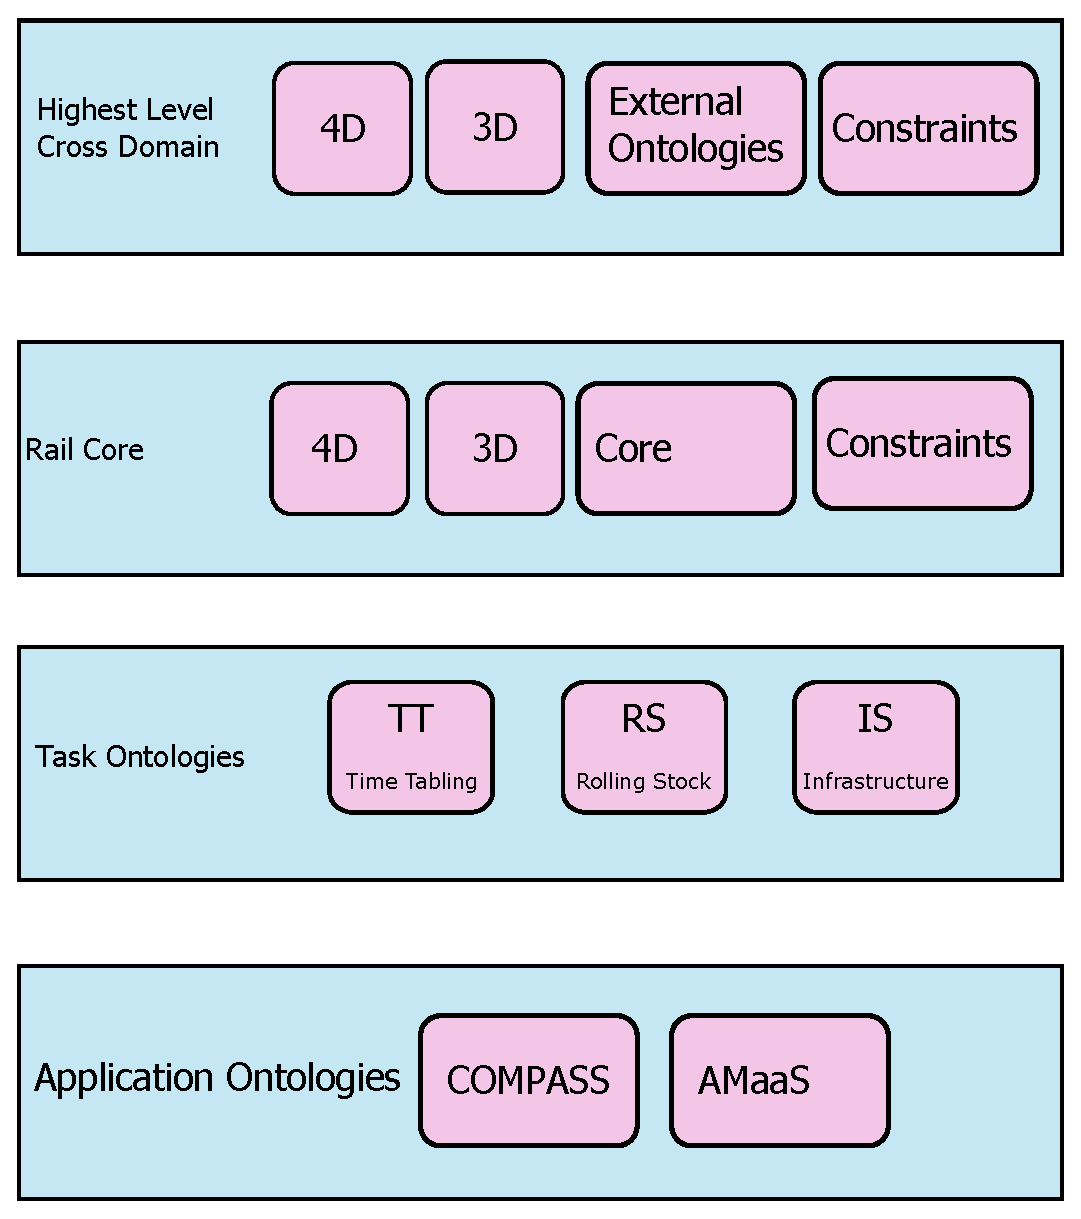
\includegraphics[width=0.6\linewidth,keepaspectratio]{gfx/RacoonLayers}}  
\caption[Racoon Layers]{Structure of the RaCoOn Ontologies. Note the constraints ontologies present on the upper two levels}
\label{fig:RacoonLayers}
\end{figure}

When RaCoOn was designed it was decided that more than one level of expressivity would be required; as stated by \citet{Tutcher2015} ``each semantic module is split into two logical modules: a ‘core’ module containing terminology, T-box relations, and other minimal semantics, and a ‘constraints’ module, containing restrictions on classes and more highly expressive constructs.''. As such the core modules comply with the OWL-RL profile and the constraints, if used, can be implemented in OWL DL, which is more complete and hence more computationally expensive. 

Note that restrictions, which require a higher level of expressivity are placed in separate ontologies which for practical purposes are contained in separate files. This are labelled \say{constraints} in \autoref{fig:RacoonLayers} This allows implementers to use only as much expressivity as their use case requires. This ontology was successful employed in a project conducted with a commercial partner, and reported in \citet{Tutcher2015a} were data from points machine and wheel impact load detectors was integrated with network layout data and a graphical interface created for it. The industrial partners in this project were then able to extend this to include circuit breaker condition monitoring, with out any further academic input. This was possible because the graphical display element had been designed to display anything that the ontology inferred to be in ``faulty'' condition, all that needed doing was declaring a new type of asset (circuit breaker) and a new fault condition (based on the time to operate). When that condition was met it was displayed in the interface with no code changes being required to the interface. 

\section{Conclusions}

This literature review has found that work is being done to remedy the poor state of data integration with in the rail domain in the UK. Data integration has been achieved in the past without use of ontology, however, significantly greater progress is possible. Much work has been done on the development of data models for the European rail domain by a range of projects, the remaining issues are now centred around the take up and use of ontology in the rail domain. Past work has shown their to be value, to many stake holders, from improved systems integration and further more it has been shown that ontology is a good means of achieving that systems integration.  Technology, tools and data models to represent the domain now exist to make implementation of ontology for data integration possible in the rail domain, as shown by the success with which it has been implemented in other domains, most notably biomedical science. 
\chapter{Problem Statement}\label{ch:probstate}
 %************************************************
Although numerous governmental and industry reports \footnote{\citep{RDG2017},\citep{DepartmentforTransport2011},\citep{TechnicalStrategyLeadershipGroup2012b}}have espoused improved data integration as a driver of reduced costs for many rail industry stakeholders and an improved travel experience for passengers, efforts towards this goal have been slow to implement. Costs would be reduced for both infrastructure and operating companies by enabling the implementation of other technologies, such as predictive maintenance which reduces their direct operating costs, along with a reduction of the cost of alterations or extensions to information systems. The benefits of predictive maintenance as discussed by \citet{QRE:QRE1634} and \citet{RDG2017}, include reduced costs by reducing unnecessary replacement of working equipment as part of planned maintenance and expensive failures caused by inadequate preventative maintenance. 

As discussed in a study commissioned by the American National Institute of Standards and Technology and carried out by \citep{Gallaher2004} the capital facilities industry (Large scale construction) in the USA projects that it could save \$15.8~billion were it to adopt ontology for data integration. Other domains have more mature implementations of ontology for data integration, most notably biomedical research where such technology is not a matter of research, but everyday use. In the consumer domain, the popular ``Siri'' virtual personal assistant makes heavy use of ontology for knowledge representation and question answering.

Previous studies\footnote{\citep{Verstichel2011a},\citep{Tutcher2013},\citep{Morris}} have shown ontology to be a useful tool for data integration in many domains, including rail, and it is this integration which makes other technologies possible. Once the range of heterogeneous datasources that many industries have, or have had, are modelled as an ontology the data contained there in can be combined and is made accessible throughout the domain. Additional benefits are possible if the rules describing how decisions are made in the domain are also encoded in the ontology, enabling better decision making and more oversight from domain experts. Ontologies already exist for the rail domain, many of which were created by the same studies as found that there would be a benefit from using ontology in the domain. The work reported by \citet{Tutcher2015}, included the design of a linked set of ontologies for the rail domain. Previously ontologies were also built as part of the InteGrail project, reported by \citet{Kopf2010}, and more recently as part of the Trapist project reported by \citet{Bhatti2016}. Additionally there has been work done in the commercial sector; notably ERTMS solutions of Brussels\footnote{\url{https://www.ertmssolutions.com/}} and Televic Rail of Izegem\footnote{\url{http://www.televic-rail.com/en/}} have done work in this area.

It can be seen that the market is starting to respond to the industry need, however there is still no significant uptake of ontologies or linked data in the rail domain. There are demonstrators, such as those reported in: \citep{Bhatti2016}, \citep{Tutcher2013} or earlier in \citep{Kopf2010}, but, in contrast to other sectors, commercial uptake remains limited. The information environment in the rail domain is very diverse and this may have impeded uptake of ontologies, as such the extent to which this is a barrier to uptake requires investigation.
In particular whilst many studies have produced data models or demonstrators there are no national scale implementations, thus investigating whether this is possible at reasonable cost would be beneficial. 

The transition from the current situation, that of many incompatible heterogeneous datasources to a system where queries can seamlessly retrieve data from multiple sources will be a complex process. It has been established by previous studies that ontology will make that possible, but the transition has not been studied in depth. Work has been done, both academically and commercially, to allow the use of relational databases with linked data and ontology. Whilst relational datasources are straight forward to convert completely unstructured data, such as technical drawings, sensor data streams, or flat text files will require further investigation. Given that tools exist to make the transition for relational data sources then it would be useful to ascertain whether it is possible to make similar tools for other data sources.

Once the transition to using ontology and linked data has been made, or even begun, another challenge must be faced, that of the skills gap in the software engineering domain centred on ontology engineering, which presents a barrier to uptake of ontology in all domains, including rail. In moving from the theoretical phase, technology readiness level 4 or 5, to implementation there is a need for both software engineers who can work with ontology datastores and ontology engineers who can construct domain models. In the long term this gap can be filled with education, however, given that neither linked data nor ontology are currently included in the syllabuses of most university level computer science courses this is not a short term solution. We should then consider whether tools could be created to help plug that gap.

If implemented fully, an ontology (or a linked set of ontologies) would hold all the logic and decision making rules used in any new software, leaving only interfaces (with humans or external equipment) to the software developer.  When creating a new interface is required, for example display on a new piece of hardware, or when a new sensor is attached to the system it would be a simple software engineering task. This would be accomplished by providing the software developer with a webservice to call which would handle the operation, thus separating the roll of ontology engineer from the roll of a software developer. By removing the specialist tasks from more generalist software engineers, the development of new systems, or modification of old, to incorporate ontologies for data storage is made possible. This eases data integration and enables all the benefits available to the rail domain discussed in \autoref{ch:litreview}.

After ontology has been applied to the rail domain another challenge to face is that of high velocity and volume data. When deployed on a national scale some data, such as that from sensors or cameras simply arrives too fast and in too large of a quantity to express as triples and store in an ontology. Such data needs to be stored separately, however more value would be available to the domain were it stored in the ontology as such, in line with the proposals in \citep{Tutcher2015}, a compromise solution is possible whereby the fine grained data resides in a suitable store and a link, along with a summary resides in the triple store. The aggregation of these storage media is a task that will need to be carried out where ever high volume sensor data is used, which is a common occurrence in the rail-domain, thus it is reasonable to ask if this could be done once to avoid unnecessary repetition.

Another problem that will be faced after ontology is adopted is that of changing interfaces to triple stores and potentially as the market evolves even changing triple stores. It would be problematic if as a new version of a triple store was released it broke existing industry software. Whilst vendors will naturally work together with industry clients to minimise this it is regrettably the case that interfaces do change with time. It is also the case that as the market matures different triple stores may present them selves as the most appropriate back-end and it would be beneficial to the industry if migration was possible. It would there for be good to investigate if it is possible to isolate the rail industry from changes to the triple stores.

The last issue this thesis will seek to investigate is that of information security. As shown in the literature review this issue is under broader consideration in the rail domain, however the question of how to secure datastores with no inbuilt security remains outstanding and is related to the question of datastore aggregation.

The questions may then be summarised thus:
\begin{itemize}
	\item \QuestionOtherData
	\item \QuestionSkillz 	
	\item \QuestionCombine
	\item \QuestionChange
	\item \QuestionCanOntologyScale
	\item \QuestionSecurity		
\end{itemize}

The remainder of this document is devoted to answering the questions above. 



\noindent
\begin{tabularx}{\textwidth}{@{}Xl@{}} 
\textsc{Question} & \textsc{Investigated In}\\ 
\arrayrulecolor{LightSteelBlue}\midrule[\heavyrulewidth]
\QuestionOtherData & \mycell{Chapter four \\ Chapter six}\\ \addlinespace
\QuestionSkillz    & \mycell{Chapter five \\ Chapter six}\\ \addlinespace
\QuestionCombine   & \mycell{Chapter five \\ Chapter six}\\ \addlinespace
\QuestionChange    & Chapter five \\                        \addlinespace
\QuestionCanOntologyScale & Chapter six \\                  \addlinespace
\QuestionSecurity  & \mycell{Chapter five \\ Chapter six} \\ 
\bottomrule
\end{tabularx}





%************************************************
\chapter{Schedule Processing Tool}\label{ch:cifparser}
 %************************************************
 \section{Introduction}
This chapter describes techniques for working with data not currently held in a form suitable for integration, but rather held, as much rail industry data is, in various single purpose formats. Methods for constructing tools to make that transition will be discussed and examples of such tools presented, alongside a discussion of when it is appropriate to build custom tools and when third party tools are appropriate. 

While ontology based systems operate on data stored as triples, it is uncommon for rail industry data to be natively stored in this form. As such tools must be provided to convert or map this data into triple based format before it can be used with ontologies. 

In the rail industry, as with most industries, much of the data currently collected and in use resides in large relational databases. Where this is the case, existing automated tools, or functionality embedded in triple stores, can be used to allow access to the data in a linked format. Other data sources, however exist in a range of single purpose formats developed as needed over time. An example of a typical industry datasource, requiring conversion is timetable information. This is required by many different stake holders, thus the benefits of it being available in a linked format will be felt by a large number of different groups such as customers for journey planning, also within the rail domain it is needed for timetable planning, train identification, crew rostering, and maintenance planning amongst other tasks. The obstacles to this transition, posed by the dated and industry specific data format as well as the volume of data are representative of the challenges that will be faced moving to ontology based systems. 

These tools present answers to the question \textit{\QuestionOtherData}. The contribution these tools make to answering the question will be assessed in \autoref{sec:cifconclusions}.

\section{Transition to Linked Data}
The transition from the existing heterogeneous systems to a more integrated solution has two parts; firstly the domain must be modelled, then tools must be designed and implemented to convert the existing data to a format which can be integrated. As discussed in \autoref{ch:litreview} ontology data is considered in two parts: the \enquote{model}, which is known as the TBox and contains the schema information and the data itself, which is known as the ABox. 

The modelling problem is being considered by numerous other studies of which the most pertinent to this work was modelling of the broader domain as part of the work reported by \citet{Tutcher2015}.  Modelling a domain requires knowledge of both ontology modelled and the domain in question, as such it can be an obstacle to transition. This challenge continues to require skilled personnel, however as more of the domain is modelled less will need modelling when new data sources are encountered. 

\subsection{Extending the ontology}
\label{sec:addingtripples}
In order as to make new datasources available as linked data it is necessary that all the concepts represented by that datasource also be held in the ontology providing the model of the domain. Where the domain ontology lacks concepts which represent the data held, it is necessary to extend the domain ontology. When this is done, it is imperative not to recreate URIs for items already in the ontology, as such the following simple steps are taken:
 \begin{itemize}
	\item Search the Tbox for URI containing the name of the property or object under consideration;
	\item Search the Tbox for URIs with labels containing the name of the property or object under consideration;
	\item Repeat the above for any common synonyms.
\end{itemize}

As is commonly stated in the literature, if an object or property (as appropriate for the concept you wish to model) exists then human judgement needs to be used to decide whether the item found is: a URI that should be reused, a super type, or different concept to that which requires modelling. Since different modelling decisions are sometimes taken at different times, it is important to check both properties and classes for any given concept. Where a concept is not directly related to the domain and may exist in an external ontology it is considered best practice to reference the external ontology rather than redefining the concept.

Once data is modelled correctly and a tool is designed to insert the abox data in an automated fashion the model will serve as a lingua franca for making the data available to other systems that require it. Additionally it will be possible to use the data in conjunction with other data stored in ontology based systems for reasoning and the abstraction of business process to rules. For example suppose a train operating company wishes to insert an extra service, for a special event at a given time and place, which attracts spectators from many separate points of origin. By combining timetable data with a static map of the network it will be possible to work out whether it is possible to add extra services from various points of origin, given also pricing information and population density data (already available in a linked format, via DBPedia\footnote{Discussed in \autoref{sec:media}}) it would be possible to ascertain the probable profit of each such service. Note that detailed routing information (not in the files discussed in this chapter) would also be necessary in this scenario. Were the ticket barriers also integrated into such a system it would be possible to sell tickets, at a price determined to make a profit and have them only work on the correct barriers at the correct stations. All of this is possible with the existing disparate systems, but many manual integration steps are required.

\subsection{Tools for processing A-Box data}

An automated tool is required to parse the A-box data in the following circumstances:

 \begin{itemize}
 	\item The data to import has some value;
	\item The data is not held in a relational format; as such automated mapping tools can not be employed;
	\item The data cannot be converted using existing tools, such as OpenRefine\footnote{OpenRefine, formerly Google refine, is a very powerful open source tool which can take data in a wide variety of formats, perform simple processing and output it again in a number of formats, including RDF. More details can be found at: \url{http:\\openrefine.org/}};
	\item Manual entry is prohibitively slow due to either the volume or velocity of data received.
\end{itemize}

Where the above criteria are met a tool to process the data and add it to the ontology is required. Such a tool would perform the following steps:

 \begin{itemize}
	\item Read the data source;
	\item Convert the data source into a logical in memory representation of that data source, generally objects representing the data structure;
	\item Iterate through the in memory representation inserting each part into the data store.
\end{itemize}

Station location data is also useful in the multi-modal domain. This information is distributed alongside the schedule data and would demonstrate how position data is best modelled. Furthermore by building tools that can process and combine multiple data sources it is possible to show the benefits of using more than one data source together. 

\section{Data to be imported}

Common interface files were selected as the source of railway data to represent in a linked format since they are representative of many formats in the rail domain that will need to be converted. Additionally since this datasource is used through out the domain its conversion will bring immediate benefits, as is demonstrated by the use of this tool and datasource as part of the demonstrator discussed in \autoref{ch:COMPASS}. 

\subsection{Legacy Resource Format}
\label{sec:datatoimport}
Currently timetables are exchanged in \enquote{common interface file} format, as defined in \citep{nr2007} first issued in June 1988 and updated regularly since to reflect changes in the UK railway over that time (not least privatisation) this is a representative example of rail data. It is neither easily human readable nor as dense as a pure binary format. Rather it uses fixed length rows of 80 ASCII characters where the interpretation of a row depends on what section it is in.

The schedule file contains the following information:
\begin{itemize}
	\item Schedules
	\item Associations (where trains are split and joined for example)
	\item TIPLOC Codes - These are one of the many ways locations are refereed to within the  UK rail network.
\end{itemize}

There is also a header row at the start of the file giving a unique ID to the file and its issue date and time, along with version information and other meta-data. The file is terminated with a trailer row, to allow users to confirm they have a complete file, though no check sum or similar is employed.

The schedule rows break down further into further subtypes:
\begin{description}
	\item[Basic Schedule] This contains header information pertaining to the entire schedule, such as the type of vehicle and branding of the service.
	\item[Origin Location] The starting point of a service
	\item[Intermediate Location]  A service calling point
	\item[Changes en Route] Where anything contained in the basic schedule field changes over the course of a trains' route.
	\item[Terminating Location] The last call of the service
\end{description}
Not all record types are necessarily present for any given service.

It is possible to ascertain not just the stopping time, and place, of a given service but also some limited meta data, including two different trainIDs, which are also used by other data sources. The first ID given is the so called \enquote{uniqueID}\footnote{the field is defined by \citet{Hicks} as \enquote{The unique ID of the schedule being activated - either a letter and five numbers, or a space and five numbers for VSTP trains}. Details available at: \url{http:\\nrodwiki.rockshore.net/index.php/Train_Activation}} which is also used by certain other systems (trust train activation messages use this ID), the second ID given is the headcode. Other systems, such as train describers and signalling systems refer to the train by this code. Whilst it is guaranteed a headcode is unique on the rail network at any given point in time more than one timetabled service can have the same headcode.

\begin{minipage}{\textwidth}%I don't want this spread accross pages
\begin{lstlisting}[label={lst:cif}, caption={CIF file example}]
BSNC821721612111712030000001 POO2S178117122832000 DMUS   075      S S          P
BX         EMY                                                                  
LOGTHM    1350 13503         TB                                                 
LIGTHMNBJ           1352H00000000                                               
LIALNGEJN           1356 00000000                                               
LIALNGNJN           1356H00000000                                               
LISLEFD   1415 1416H     141514161        T                                     
LIHCKNGTN 1423 1423H     14231423         T                                     
LIHBRTBDG           1432H00000000                         2                     
LIBOSTON  1441 1445      14411445         T                                     
LISIBSEY            1452H00000000                                               
LIBELWTRJ           1459 00000000                                               
LIWAINFLT 1508H1509H     15091509         T           2                         
LTSKEGNES 1521 1524      TF                                                     

\end{lstlisting}
\end{minipage}

Each row starts with a 2 letter code to uniquely identify the type of data it holds and some row types are only valid in certain places. For example each train service definition starts with a basic schedule row, then an origin location, followed by any number (including zero) of Intermediate Location's or Changes en Route and finishing with a Terminating Location. An example is shown in \autoref{lst:cif} of a complete, but short schedule in this format. Note that the schedule starts with a `BS' or ``Basic Schedule'' line, then goes on to list calling points, with the last listed as  `TF' train finishes. The time format is twenty-four hour and the presence of an `H' after a time means ``and a half'' hence 1352H should be read as ``13:52:30''. Thirty seconds is the maximum accuracy this format allows for. 

These files can be used in conjunction with a \enquote{Master Station Names} file which is typically distributed at the same time. This file provides further detail about the stations refereed to in schedule. Whilst TIPLOC codes are listed in the schedule file alongside a meaningful name in English, the geographic position for example is not provided. This is included in the master station names, alongside side details of the type of services that may be connected with (bus or ferry for example) and the Routing Groups, which are used for fare calculation. By joining on the TIPLOC code it is possible to combine this data with that in the schedule file.

The size of the files to be imported also represents a significant test: the chosen schedule file was 564MB, in what has already been described as a fairly dense data format. This will result in a significantly larger amount of data if exported as turtle, which is a simple text representation of linked data, presenting challenges in terms of both processing time and available RAM. As such the system will need to be carefully optimised to fit within the memory footprint of a workstation-pc (24 GB in this case).

\section{General Software Design Patterns}
Two design patterns were considered for a system to parse schedule files: a state machine and a factory pattern. The state machine pattern, as set out by \cite{Shalyto2006}, provides loose coupling between the logic of the program and the state, which is considered through out the literature to be a key objective of any software architecture. The transition logic required for processing schedule files is very limited and thus the state machine pattern was disregarded as unnecessary in this application. The factory technique first discussed in \cite{Gamma2002} conversely is applicable to this system since it abstracts the construction of objects from the point at which they are created. This is helpful in this system since it is likely that further types of data and therefore business object will need to be added to design in the future. The system aims to be flexible as to the types of files parsed, importing both \enquote{Master Station Names} files and Schedules, using the same architecture. In the factory pattern \enquote{factory classes} are used to construct objects, rather than calling an object's constructor directly. Currently there exist two factory classes, one for each type of file processed, which build the business objects before they are inserted into the datastore. A deliberate benefit of the design is that it is easily possible to add more as required.

The graphical user interface (here on referred to as GUI) partially uses the Model View View-Model design pattern, here on referred to as MVVM, to loosen coupling with the data processing part of the application. The MVVM pattern is described by \citet{Microsoft2012} and is a common way to create GUIs when using the Windows Presentation Foundation. The Windows presentation foundation in turn is a means of creating GUI's when using the .Net framework on windows desktop machines. The MVVM pattern aims to reduce coupling between the designed user interface, which is created using only XAML and describes \emph{solely} appearance (include  interactive elements such as mouse over animations) and the way the data is formatted for presentation. In this pattern the data model is independent the view model.  Data representation and processing is removed again, thus changes to how data is presented (say from a table to a graph) have no impact on the underlying system.

\section{Software implementation} 
The schedule processing tool is designed in keeping with object orientated best practice, namely: SOLID\footnote{A good explanation of SOLID design principles, illustrated with motivational posters, may be found at \url{https:\\blogs.msdn.microsoft.com/cdndevs/2009/07/15/the-solid-principles-explained-with-motivational-posters/}} software design principles, as first set out by \citet{Martin2003}. An example of the schedule processing tool's structure and inheritance is shown in \autoref{fig:tiplocedItems}.  

 \begin{figure}[!h]
\myfloatalign
{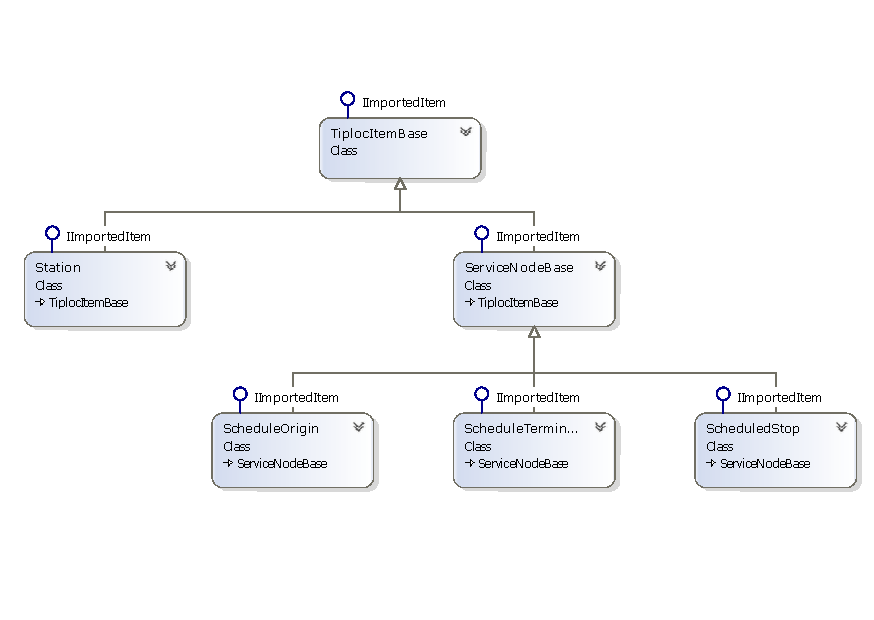
\includegraphics[width=\linewidth]{gfx/ItemsWithTIPLOCsResized}} 
\caption{Items located using a TIPLOC - one of the location codes.}
\label{fig:tiplocedItems}
\end{figure}

The business objects represent the data contained in the file, at a low level, both row by row and at slightly higher level representing schedules. All low level business objects implement the same interface, allowing for their population (from a string representing an entire line) as well as providing methods which allow for storing them to a graph. There exists a factory object for each file type parsed by the system (others can be created as needed) which handles the splitting of the source file into lines, for the creation of business objects and in particular for handling objects which are split across multiple lines, such as schedules. The business objects and the factories that create them are shown in \autoref{fig:bo}.

As a result of this design should a new file type need to be imported the tool could be extended without changes to the existing code. A framework both for reading files into memory and for inserting them into a triple stores is provided.

\begin{figure}[!h]
\myfloatalign
{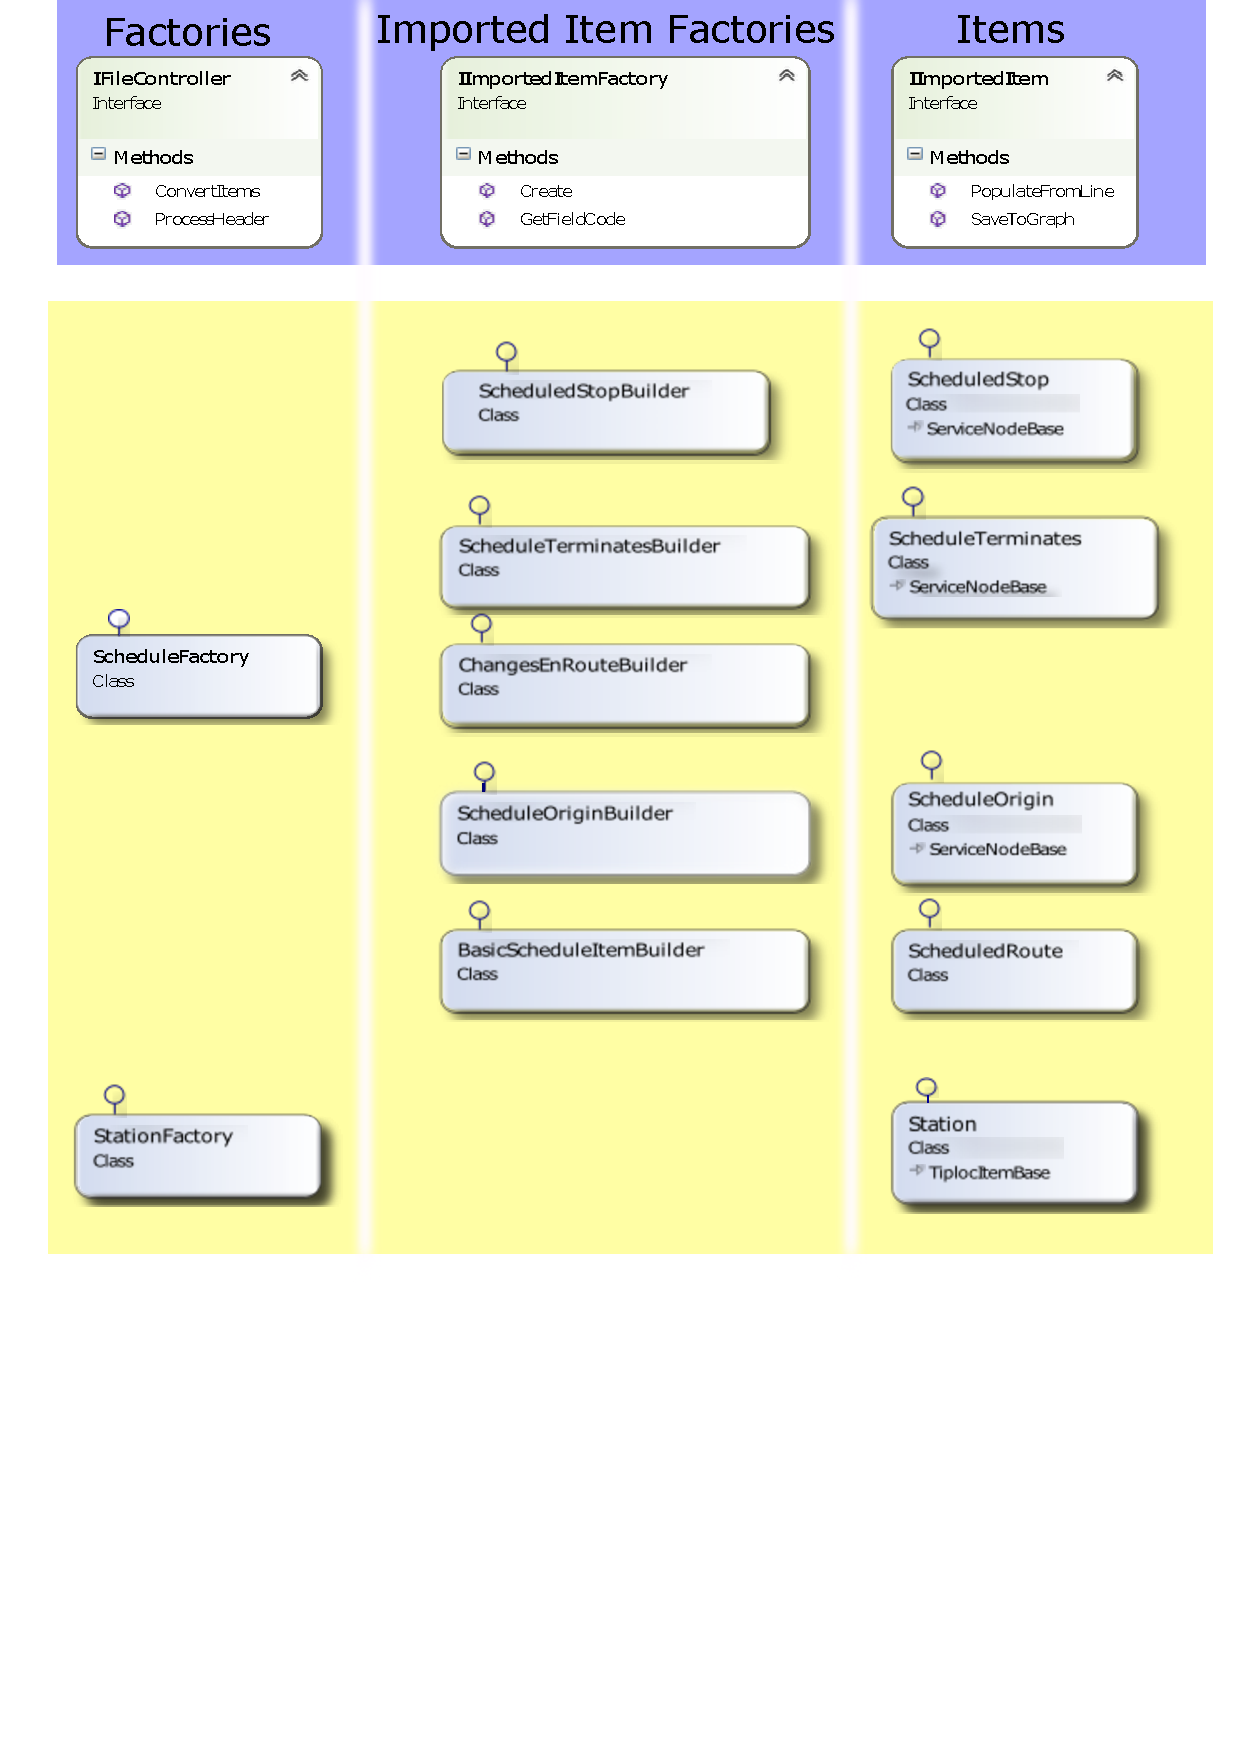
\includegraphics[width=\linewidth]{gfx/BussinessObjectsCat}} 
\caption{Business Object inheritance}
\label{fig:bo}
\end{figure}

When the business objects had been created it became apparent that some of the data they modelled was not modelled by the ontology. These fields were then added as properties in accordance with the guide lines set in \autoref{sec:addingtripples}.

Another .NET practice embraced in this project was the use of the provided settings mechanism for storing constants. This allows for changes to the settings when ever they are required as well as keeping the settings within source control and in one place for easy editing. 

An open source third party library, dotNetRD, was used for connection to local and remote triple stores. This library also allows the construction of graphs in memory and makes it possible to perform reasoning on them. This library was chosen using the fulfilled criteria:
\begin{itemize}
 \item Active maintenance;
 \item Open source (hence free to use);
 \item Compatible with the other technologies in use, in particular C\#.
\end{itemize}

It was discovered in implementing this project that when dealing with very large graphs, as was the case for schedule data, it is necessary to prevent the framework from interning all of the Uri's added as this whilst this has performance benefits they come at the cost of an enlarged memory footprint.

Given the data volumes involved it was necessary to identify bottlenecks and tasks that could be carried out in parallel and run these on separate threads. The machine used for both development and bench marking has the following pertinent specifications:
\subsection{Hardware Specification}

\noindent
\begin{tabularx}{\textwidth}{XX} 
\toprule
\textsc{Item} & \textsc{Specification}\\ 
\arrayrulecolor{LightSteelBlue}\midrule[\heavyrulewidth]
Processing & Intel i7-3820\footnote{Intel Data sheet available from: \url{http:\\ark.intel.com/products/63698/Intel-Core-i7-3820-Processor-10M-Cache-up-to-3_80-GHz}} @ 3.6 GHz. This has 4 cores and can run 8 simultaneous threads. \\
Random Access Memory & 24 Gigabytes \\
Disk & Two Terrabytes, average data rate (Read and Write) of 156 MB/s. \\
\bottomrule
\end{tabularx}
 
The graphics card fitted was of no assistance because none of the tasks in this program were suited to offload to the graphics card.

Bottlenecks were identified by running the \enquote{Performance Profiler} included with Visual Studio on the initial version of the software. This can tell the operator which objects are using most of the memory and which functions the schedule processing tool spends longest in. It was apparent from this that most of the memory usage was in the graph constructed by dotNetRDF and most of the processing time was in constructing that graph. In order as to achieve adequate performance, that is to be able to run an import whilst the data is still pertinent, a multi-threaded approach was required. To achieve this the data was split into chunks, after having been read from the file, but before it was materialised as a graph. Each chunk represented 500 individual elements from the underlying file, expect for the last chunk, which contained as many elements as were left. This reduced the memory footprint, since the graph was only created one chunk at a time, then stored to a file and the memory it had been occupying released. This approach also made parallel processing possible, as each chunk could be (and was) materialised separately. This design could scale linearly with the number of cores available. In order as to accomplish the multi threaded materialization and writing it was necessary to create a thread pool of data waiting to be processed and written. This uses .Net's underlying thread-pool provision but adds progress feedback and ensures that files are only written after the data is processed. The data was output as a series of turtle files, which were then inserted into a triple store using a script. This work-flow is illustrated in \autoref{fig:workflow}.

\begin{figure}[H]
\myfloatalign
\fbox{{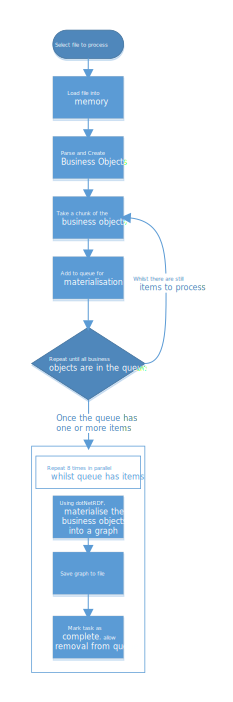
\includegraphics[max height=\textheight,max width=\linewidth]{gfx/cifParsingWorkFlow}} }
\caption{Data conversion work-flow}
\label{fig:workflow}
\end{figure}

The graphical user interface is simple and shown in \autoref{fig:cifgui}. All that was required was status feedback, for use debugging and to inform the user when the conversion was complete, and buttons to select the files to import. Also available is functionality to add provenance information to the schedules. Provenance information is added to the data when it is inserted in the ontology, allowing the source of the information to be traced, in accordance with the guide lines set out by \citet{Tutcher2015}.

\begin{figure}[H]
\myfloatalign
\fbox{{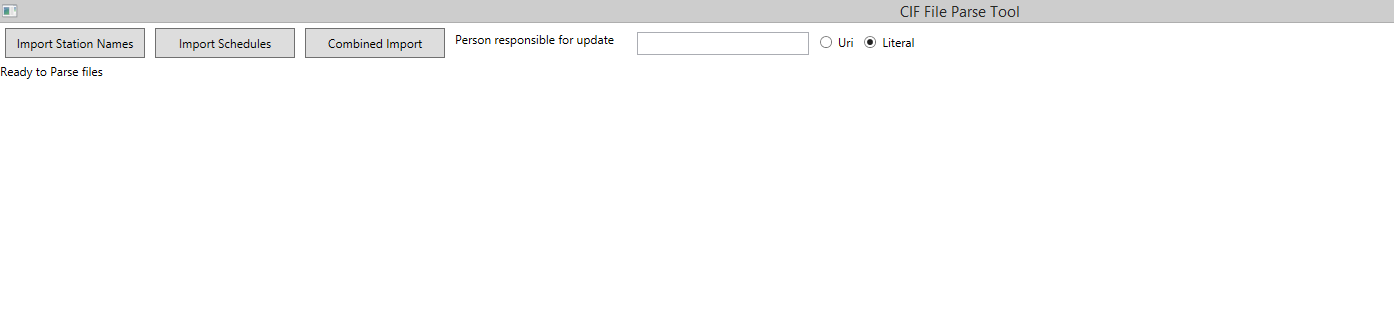
\includegraphics[max height=0.5\textheight,max width=\linewidth]{gfx/cifparseRelevantCorner}} }
\caption{Schedule parsing tool interface}
\label{fig:cifgui}
\end{figure}

\section{Manual Data Entry Tool}
\label{sec:manualtool}
The manual data entry tool demonstrates a technique for adding previously modelled low volume data to the ontologies. Where such data does not warrant the development of a bespoke tool for the task and it is not possible to interface with or alter the existing tool then a simple universal tool allowing those with no ontology engineering experience to add data to the ontology allows for improved data integration. There are many pre-existing ontology editors, both open source and commercial, of which protégé and TopBraid Composer were used during this project, however these are better suited to those with some ontology engineering experience. This tool is aimed at those with no ontology engineering experience and thus provides another possible answer to the question, \enquote{\QuestionOtherData}.

\subsection{Manual Data Entry Tool: Implementation}
The tool was constructed as a web application, with intent that it could be deployed centrally in large organisations and used as needed. This tool relies upon the middleware, discussed in chapter \ref{ch:middleware}, to connect to the triple store. For layout and presentation the popular \enquote{bootstrap}\footnote{Available from: \url{https:\\getbootstrap.com/}. This framework provides a number of styles alongside Javascript functionality} framework was employed to speed development and allow for access from a range of devices.

 \begin{figure}[H]
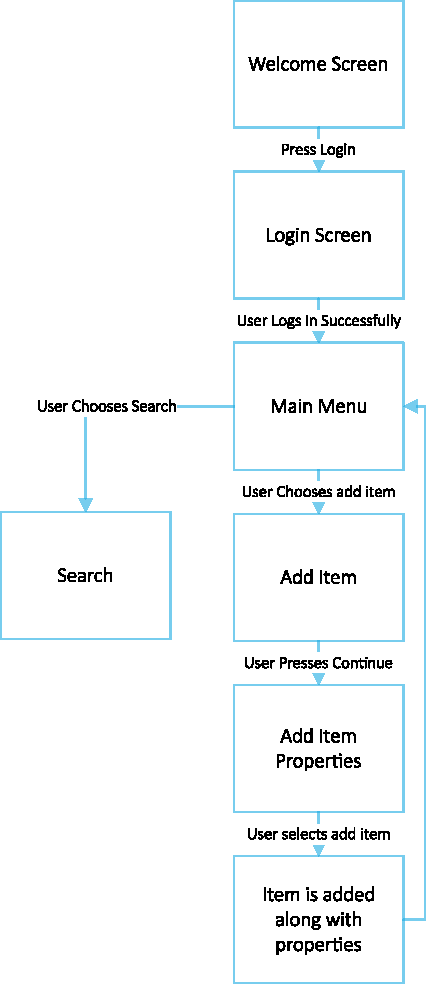
\includegraphics[max width=\linewidth]{gfx/manEntryWorkflow}
\caption{Manual Data Entry tool work flow for adding individuals to the ABox}
\label{fig:mtWorkFlow}
\end{figure}

The main menu presents user with the following options:
\begin{itemize}
    \item Adding new individuals
    \item Viewing individuals
    \item Uploading data, related to specific project, namely COMPASS as discussed in \autoref{ch:COMPASS}. 
\end{itemize}

The procedure for adding new individuals is set out in \autoref{fig:mtWorkFlow} and shown in the screenshots available in \autoref{app:mantoolgui}. In \autoref{fig:mtAddingItemDetail} (in  \autoref{app:mantoolgui}) the mechanism for supplying values for any properties that are expected is shown, the properties displayed are selected based on those that other individuals of the same class have. Users are free to enter a value or not for all of the properties shown. When done the data is then stored in the ontology.

\section{Results} 
Initial tests, on the unoptimised system, were performed with smaller schedule files, truncated to 64MB, from an original 564MB. Chunks of this size took more than twelve hours using an unoptimised version of the software, when full files were processed the program ran out of memory before returning results.

The final version of the software took two minutes and thirty four seconds to complete a cut-down (64MB input file) run. The full run took 06:46:36, which indicates that further optimisation remains possible, however this time frame would be usable.  

The files were quickly and successfully inserted into the triple store (stardog), where the inserted RDF was verified as consistent. 

As can been seen from \autoref{fig:cifparsing} in the optimised version performance is non-linear with time, and as the limit of system memory is approached performance degrades significantly. A summary of the data illustrated by \autoref{fig:cifparsing} is available in \autoref{tab:cif}, which again shows that as the system consumed most of the available memory performance was significantly degraded. Through out the testing debugging tools stated that the tool alone used approximately 22 of the available 24 Gigabytes of RAM in the test system. The non optimised version was never run to completion, but had reached approximately 50\% completion after four days. 

The system also output the time taken to perform the various parts of the conversion. Converting the business objects to an RDF graph, using dotNetRDF took over five hours, where as reading the file from disk and converting it to simple, lean, business objects took twenty six seconds, which clearly indicates where the processing was required.

{\parindent0pt
\begin{figure}[H] %I don't want this figure miles away, acept having some blank space
\centering
\subfloat[Turtle files processing time graph\label{fig:cifparsing}]{%
\adjincludegraphics[width=1.3\textwidth,center]{gfx/FilesEvery15}
%\caption{Turtle files processing time graph}
%\label{fig:cifparsing}
}
 
\subfloat[CIF processing times, by hour\label{tab:cif}]{%
\begin{tabularx}{4in}{@{}cc@{}} 
\arrayrulecolor{LightSteelBlue}
\toprule \\
\textsc{Hours from Start} &  \textsc{Number of Files Produced} \\
\midrule[\heavyrulewidth]
1 & 306 \\
2 & 278\\
3 & 52\\
4 & 55\\
5 & 43\\
6 & 35\\
7 & 45\\
8 & 11\\
9 & 0 (complete)\\
\bottomrule
\end{tabularx}
%\caption{CIF processing times, by hour}\label{tab:cif}
}
\caption{Time to output turtle files}
\end{figure}
}


The source code for this tool is available at: \url{https:\\github.com/Chris-MorrisUK/CifParser}.

\section{Conclusions}
\label{sec:cifconclusions}
This system was created in response to the following question: \textit{\QuestionOtherData}

Firstly this system has shown that it is possible to make typical industry data sources available in a linked format, by taking schedule data, a typical industry data source and making it available as turtle files, which can be loaded into a triple store and queried or reasoned over. 

Secondly this system has shown that even quite small data sources, as compared to video or high data rate sensors for example, require a high degree of optimisation and produce much larger data sets in a linked format. 

This design and implementation of this system also demonstrated that even where the domain has been partially modelled new applications of that model will require small alterations to suit the precise nature of the available data and its eventual use. This in turn has wide ranging implications for the need for ontology specialists to be involved, lightly at least, in the design phase of future projects making data available as an ontology. This in turn has relevance to the question: \textit{\QuestionSkillz}

The manual data entry tool provided another answer to the question \enquote{\QuestionOtherData}. For some projects the production of bespoke tools will not be financially justifiable. Where it is not possible to use commercial off the shelf software to convert data and that data is of a low enough volume then it will be possible instead to use tools to manually enter that data.

This system has also made it possible to explore: \textit{\QuestionCanOntologyScale}

The data imported covered the entire UK rail network and whilst it would have required running overnight it was none the less functional. Were the solution to be reworked so as not to create a graph of the data, then store it as turtle, but rather to directly interface with the triple store it may be possible to reduce the running time further.

\section{Further Work}
This tool could be directly connected to a datastore, thus not generating an in memory graph and serialising this to turtle files which then require insertion. This may well allow for faster processing and a smaller memory footprint. 
%************************************************
\chapter{Use of a Middleware Layer with Ontologies}\label{ch:middleware}
%************************************************
\section{Introduction}\label{sec:mwintro}
The benefits of adopting linked data and related techniques, even in environments with substantial legacy resources are clear. In essence this is achieved by first modelling the schema of the data, then making the ABox (row) data available to the ontology. Once an area or sub-domain has been modelled, software must be developed that allows software and services within the industry to interact with the the data in the triple store. This currently requires specialist knowledge, not common in the software engineering community, and this gap presents another barrier to industrial implementation of ontology based systems. As a minimum a developer working in the area would need a detailed understanding of:
\begin{itemize}
    \item SPARQL;
    \item XML data types;
    \item The APIs for the triple store to be used.
\end{itemize}

In addition to these, for the knowledge of the specific technologies to be of value, a certain amount knowledge of higher level ontology principles is required. At the very least a familiarity with triples and, in an environment where reasoning is used, inference is also required. It is reasonable to expect that most professional software engineer will have some knowledge of XML data types, on that basis it should be possible for them to learn the basics required to interact with the triplestore within the lifespan of any large industrial project, learning SPARQL or higher level concepts will take significantly longer.

Whilst it is likely that in the long term the skills gap around ontology will be filled by improved education and training in the short and medium term the adoption of ontology linked data in the rail domain would be considerably accelerated by the production of tools that enable software engineers without ontology experience to interact with data stored using an ontology. The RaCoOn middleware exists to bridge that gap.

\subsection{Roles}
The RaCoOn middleware exists as an intermediary between the triple store holding the ontologies, and applications that require access to those resources. In addition to enabling this simple connectivity the middleware also provides and manages connections to REDIS, a key value store used to handle high frequency data, and adds a security layer. Applications use the middleware via Windows Communication Foundation (WCF) web services, which where ever possible implement RESTFul design principles. The middleware represents several contributions to ontology development for the railways: Firstly it acts as a \say{buffer} between the triple store and the connected applications (consumers). Different consumers have a range of access requirements and as the market evolves it is possible, even likely, that the selection of commercially available triple stores will change. The middleware ensures that as the software components on either side of the middleware evolve the larger system is unaffected; the same interface will be presented to the consumer regardless of the choice of triple store. Another key benefit the use of a middleware offers, is the ability for developers to easily interact with a range of specialist datastores as needed by the application use case alongside the triplestore itself. In the scope of this document, this is illustrated using the REDIS key-value store as a lookup for high frequency data streams, however, as the technology develops many other similar storage needs are likely to be identified.

Since some data stores don't have their own security, an additional benefit of the middleware is a single sign on and token system can be handled by the middleware.After a user is authenticated by the middleware and given a token allowing continued access all datastores behind the middleware are accessed using that token, regardless of the security mechanism they employ. For systems that have complex access control hierarchies it is possible to map each user signing on to the middleware to their unique username, whilst systems bereft of security can be shielded from outside access. 

By using a middleware common functions shared by a number of applications can be implemented at this level avoiding duplication. The WCF webservices make it possible to connect to the middleware using clients written in most common languages and from most environments, allowing developers to use the best tool for the current project. The overall architecture is summarised in \autoref{fig:MiddlewareHL}.

\subsection{Data Volumes}

A major challenge to the migration from the current ecosystem of mixed incompatible data stores to one that embraces linked data and ontology, is that of data volumes. Whilst the market for triple stores has moved forward significantly in the last five years and a number of triple stores will now scale to significant volumes of data when run in an appropriate environment, triples are an inherently inefficient way to store most types of data. High frequency data streams, which are common in industrial applications, such as remote condition monitoring, are particularly difficult to handle in most triple stores due to the computational overhead associated with rapid updates. \citet{Tutcher2015} mitigated this problem by supplementing the triple store with REDIS, which acted as a buffer for the high frequency data.

The triple store holds a summary of the data along with a link which can be used to retrieve it from another store. For example where a complex wave form is recorded, its amplitude, duration and the time at which the sample was taken could be stored as triples, alongside a key to retrieve it from REDIS. REDIS is highly optimised for fast retrieval of large amounts of data using a very simple key, deliberately leaving security entirely to the user.

 \begin{figure}[H]
\myfloatalign
{\includegraphics[width=\linewidth]{gfx/Middleware_role}} 
\caption{The role of the Middleware}
\label{fig:MiddlewareRole}
\end{figure}

\section{Functionality}
 \label{sec:function}
For the middleware to provide the services shown in \autoref{fig:MiddlewareRole} it must provide a number of functions:
\begin{itemize} 
    \item Brokering: acting as an intermediary between client and server;
    \item Datastore aggregation;
    \item Provision of stored procedures;
    \item Provision of datastore security;
    \item Provision of common functionality.
\end{itemize}

Each of these will be discussed in the following sections.

\subsection {Brokering: acting as an intermediary between client and server}
The middleware must act as a broker or intermediary between applications consuming and contributing to datastores. One of the challenges the industry will face during a transition to linked data is that as the datastores available evolve with time, and new technologies are developed the interfaces the datastores present will also change.

In an established industry it can be expected that new client applications will be created on an as needed basis when required for a project. This will likely be over an extended period, probably measured in years and there will be no \say{big bang} style switch-over event in which the entire industry is migrated over to linked data over night. 

Suppliers are starting to respond to the industrial need for easier to use interfaces to triple stores, and SPARQL has existed as a constantly evolving standard query language for some time; however this alone does not alleviate the risks of vendor lock in when choosing a triple store, and thus the provision of intermediaries between the data store and the end user applications is certainly prudent, if not necessary.

\subsection{Datastore aggregation}
New datastores are being developed rapidly as the technology matures, all with different strengths and weaknesses. As the market evolves it is possible, even probable, that new railway projects will require access to different types of data store, in keeping with the project's needs. In the first instance REDIS has been selected as a second data store to make available, since this has been used in previous projects with RaCoOn for high frequency data. Many railway condition monitoring applications, such as alternating current field measurement sensors to detect cracks in rails, or laser distance sensors, as used in condition monitoring of railway assets can generate very high volumes of data.
\subsection{Stored Procedures}
The middleware provides \say{Stored Procedure} functionality similar to that commonly found in relational databases. This has several benefits, applicable to both relational data stores and this system:

\begin{itemize}
    \item Improved reuse. Once a stored procure has been written it can be used by many systems, or the same system in many places with out rewriting it;
   \item Isolation between the software and the query. As such if the representation of the data changes only the query need change, not the system using it. In the case of ontologies, as opposed to relational databases, this should only be relevant if major re-factoring is done for example if a different domain had to be used for all URI's in the system.
    \item Familiarity for developers used to a relational database environment;    
    \item Less data needs be sent to the middleware since the name of the stored procedure is much shorter than the SPARQL required to describe the query. 
\end{itemize}

By providing a familiar mechanism to developers coming from a relational database background, the middleware reduces the learning curve for those new to the technology. Other benefits from the relational database domain are less applicable to the linked data domain, in particular the stored procedures can't be pre-compiled for faster execution, since the middleware is not responsible for the compilation of the query.

Stored procedures created in the middleware can seamlessly use any datastore, there is no difference to the user and no changes to the implementation need be made when a different store is used, though it is likely that the stored procedure will need to be updated to match the API provided by the new store. Application code which has been developed to use one data store via the middleware will continue to do so transparently when another is added. 


\subsection{Information Security}
Information Security has become an important research topic recently, as the possibilities of electronic crime and attacks against infrastructure are considered.

The question of information security is a broad topic, and it is beyond the scope of this thesis to address it in its entirety. It is however necessary to investigate the impact on information security of moving to a system of linked data and ontology.
It is common in the literature to divide information security challenges into three areas: 
\begin{description}
    \item[Confidentiality] Presenting the improper disclosure of information as considered by \citep{Erlingsson2016};
    \item[Integrity] Insuring that information remains accurate;
    \item[Availability] Ensuring that information remains available in all circumstances. 
\end{description}

Triple stores are reaching a level of maturity similar to that of relational databases, this includes the ability to cluster for both improved scalability and availability. Running triple stores in a virtualised cloud environment can also result in increased availability of data. 

When considering information integrity, ontology allows the insertion of provenance information, making it possible to understand why any given change was made to the data. Whilst it has not be implemented, in this work, at the middleware level it should be possible to include functionality in the middleware to automatically append provenance to data as it was inserted. 

The most significant contribution the use of the middleware makes to information security can be found in confidentially. By imposing a secure layer between the unsecured data store and the wider network (or indeed internet) the middleware prevents unauthorised access to other datastores. Taken in conjunction with the datastore aggregation this approach has the added advantage of providing a ``single~sign~on'' for all datastores. The trusted component, in this case the middleware, is accessible from client machines however all hosts running datastores trust \textbf{only} the middleware and not the larger network. 

\subsection{Centralising Common Functionality}\label{midfunc}
In an ontology architecture using middleware common functionality may be moved into the middleware to avoid needless repetition in keeping with the software development doctrine of \say{Don't Repeat Yourself (DRY)}. This centralisation of functionality can make clients lighter weight and less time consuming to develop. The middleware must also implement functionality to handle security and to query the data stores the middleware connects to, both using stored procedures and queries. The following functionality is commonly needed by systems connected using an ontology for data storage:
\begin{itemize}
    \item Free text search of individuals within a class, using the label text;
    \item Get all individuals of a given type;
    \item Add new items.    
\end{itemize}


\section{Middleware Design Patterns}
When developing an ontology architecture the techniques used to link client applications to datastores are similar to those faced in any other domain of software engineering. 
The design of this software employed several common software engineering techniques for example, where exactly one instance of a class was required, such as connecting to a datastore, the \say{Singleton} pattern was employed to ensure only one instance was ever created. Additionally in order as to prevent repetition of code SOLID principles (previously discussed in \autoref{ch:cifparser}) were employed.

\section{Implementation}
In order as to provide the functionality set out in \autoref{sec:function}, the middleware was implemented as collection of webservices, using the windows communication foundation (WCF). These can be consumed by clients created using a range of development techniques, and libraries exist to aid connection to WCF webservices from several languages, however it is most common to use the .Net family of languages for the client.

\subsection{Modular Structure}
The middleware solution contains the following modules:
\begin{description}
    \item[RacoonMiddleware] Holds the Webservices and calls the other projects as needed;
    \item[MiddlewareBussinessObjects] Holds representations of objects referred to by the ontology as C\# objects;     
    \item[REDISConnector] Acts as the intermediary between the middleware and REDIS.
    \item[StoredProcCreator]
    This module compiles to provide a simple graphical (Win32) interface for creating and editing stored procedures. 
    \item[StardogConnection]  Acts as the intermediary between the middleware and Stardog.    
    \item[UploadLDLTool]
    This module compiles to a very simple graphical tool (Win32) for testing the processing of LDL files, required for a specific project which is set out in  \autoref{ch:COMPASS}. It is not intended for production use, rather it was a debugging tool before the functionality had been added to another system.
    \item[UserManager]
    This tool manages the users that have access to the middleware. It is a small, simple tool for use by system administrators.
\end{description}

The relationship between these modules and external modules is shown in \autoref{fig:MiddlewareHL}.

\begin{sidewaysfigure}
\myfloatalign
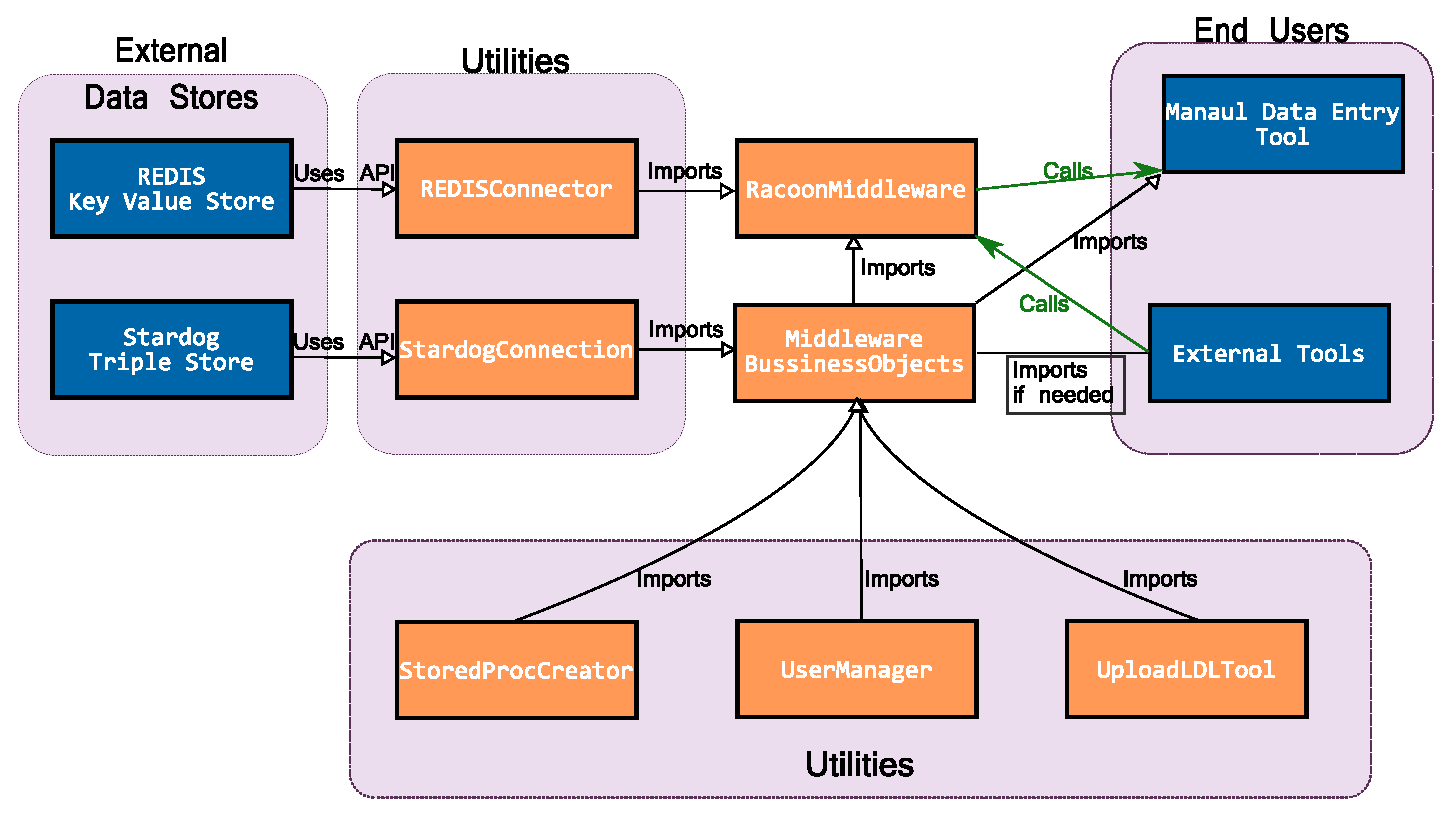
\includegraphics[max height=0.9\textwidth]{gfx/MiddlewareHighLevel}
\caption{The interactions between the middleware modules, both internal and external}
\label{fig:MiddlewareHL}
\end{sidewaysfigure}

\subsection{RacoonMiddleware}
\label{sec:middlewaremodule}
This module contains the webservice definitions and the functionality directly related to them and thus is the part of the middleware with which external developers will interact directly. In particular it contains definitions of all the responses that can be given by the webservices and all the parameters accepted.

In keeping with software engineering best practice, for systems providing many similar functions, this module in particular makes heavy use of SOLID design patterns. \\ All of the responses returned by the webservice extend a simple base class entitled \say{\texttt{SimpleRacoonResponse}}, which provides the basic details every response from the webservice will include, namely:
\begin{description}
    \item[AuthorisationOK] A Boolean value indicating if the token provided was accepted. If this is false then the token is not valid. The most probable cause for this is the token timing out, since they are only valid for a given length of time, currently configured as one hour.
    \item[Error] An exception, if this is not null an error of some kind has occurred. The message should be suitable for display to a user and the type of the exception should be informative.
    \item[Status] If this is true the operation completed successfully and the results can be replied upon. If it is false then the results should be discarded. 
\end{description}

This inheritance is set out in \autoref{fig:MiddlewareResponses}, which also gives details of the possible response types. The response classes in turn all either implement one of the interfaces set out in \autoref{fig:ResponseInterfaces} or a extend a class that does. This was in keeping with good object orientated design practice, since every response requires some common authorisation and error handling functionality as set out above and it allows the system both handling and generating those responses to be written once, not rewritten for every webservice.  Inheritance was also used by the classes implementing the webservices, in keeping with the principles of reusing code rather than copying it, as shown in \autoref{fig:services}.

\begin{sidewaysfigure}
\myfloatalign
{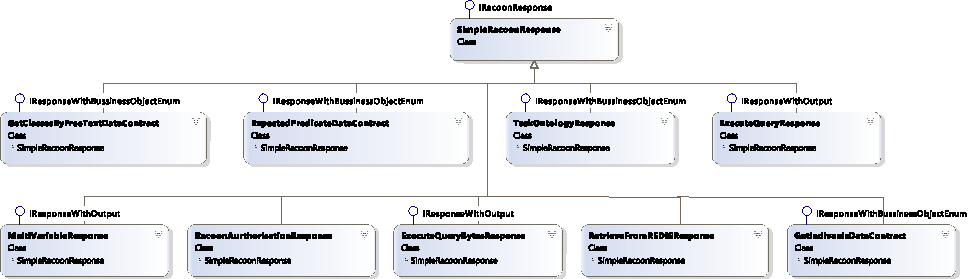
\includegraphics[width=\paperwidth]{gfx/MiddlewareServicesClassesResponseOnly}} 
\caption{The response types returned by the RaCoOn Middleware}
\label{fig:MiddlewareResponses}
\end{sidewaysfigure}

 \begin{figure}
\myfloatalign
{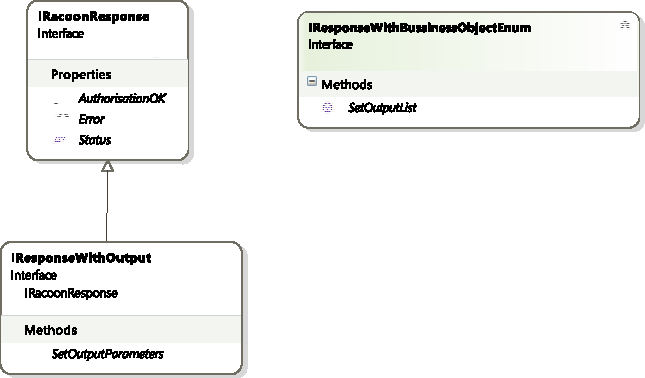
\includegraphics[width=\textwidth]{gfx/Res}} 
\caption{The interfaces implemented by webservice responses}
\label{fig:ResponseInterfaces}
\end{figure}

 \begin{sidewaysfigure}
\myfloatalign
{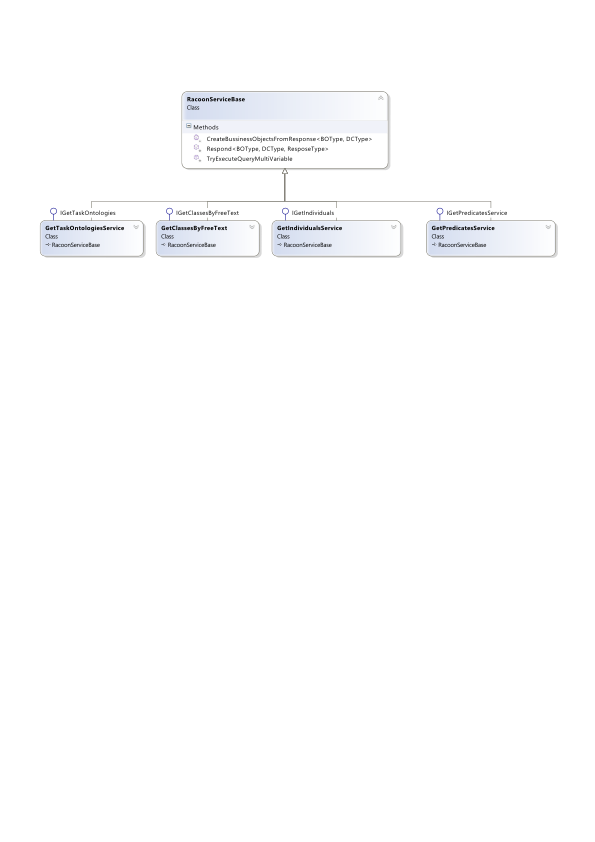
\includegraphics[width=\paperwidth]{gfx/RacoonServices}} 
\caption{Selected webservices}
\label{fig:services}
\end{sidewaysfigure}

The \texttt{RacoonMiddleware} module is also responsible for acting as an \say{intermediary} between multiple different data stores. Within the framework discussed Stardog is used as the main datastore (the triplestore), with REDIS support included to provide a buffer for high velocity data streams. However the framework is flexible and would allow for the addition of extra datastores with no impact on the existing stores or the framework. In order as to isolate this datastore specific code from the rest of the system it is implemented in separate Dynamic Link Libraries, here on referred to as DLLs. This allows for; the easy addition of new datastores, reduced regression testing when the DLL is changed to match changes in triple store interfaces and logical separation from unrelated code. In order as to be usable by the larger system the DLL must make available or \say{export} an implementation of the interface set out in \autoref{lst:query}. Stored procedures have a field setting out the fully qualified name of the stored procedure's type, as seen in \autoref{lst:StoredProcedure} so if the DLL is in memory all that needs be done to access a new datastore is create a stored procure with that type specified and it will be used, with no code changes to this module. 

\vfill
\begin{lstlisting}[language={[Sharp]C},frame=tb,caption={The IQuery interface, which must be implemented by all executable queries},label=lst:query]
/// <summary>
/// An abstract query, targeting any data store. Includes methods for setting any variables included in the query
/// </summary>
public interface IQuery
{
    void SetTarget(string server,string datastore);
    void SetQuerry(string queryText);
    IEnumerable<MiddlewareParameter> Execute(IEnumerable<MiddlewareParameter> parameters, Session session, ParameterTypeEnum returnTypeWanted);      
}
\end{lstlisting}

As can be seen from \autoref{lst:query} queries and stored procedures managed via the middleware can take any number of parameters, which can be one of several types:

\begin{description}
    \item[Uri]  Unique Resource Identifiers, as used in linked data;
    \item[String] String data and all other data types not specifically handled;    
    \item[Byte] For transferring binary data.
\end{description}

This list can be expanded if needed. These restrictions only apply to stored procedures and to functions directly passing queries. Task specific webservices can take or return any type including a business object related to the operation they perform, or a simple in built types.

This system of stored procedures can have a significant impact on the ease of integration of software systems. This also makes it possible to demonstrate how stored procedures can query multiple data stores. As such they are implemented within the  \texttt{RacoonMiddleware} module, \autoref{lst:StoredProcedure} shows the implementation.

An XML file, holding numerous instances of the class shown in The implementation of the stored procedures is included in \autoref{app:spList} in \autoref{lst:StoredProcedure} provides the database of stored procedures. For efficiency this is read into a dictionary in memory on start-up then stored procures are retrieved, using a hash of the stored procedure's name as its key in the dictionary. This allows for very fast access to stored procedures, which is necessary when dealing with high velocity data, such as that from sensors.

\subsection{MiddlewareBussinessObjects}
Modelling real world data in object orientated programming as \say{Business Objects} is a staple programming technique when dealing with conventional data storage. Typically the business objects either hold only instance data, in which case it is known as an \say{anaemic domain model}. The alternative, putting business logic and validation in the business objects is known as a \say{rich domain model}. Where ever the restrictions are placed, be they in the domain model or in another layer, this is where traditional developers model the domain. When using ontologies both the model and as much as possible of the business logic belong in the ontology, however, in order as to work with this in a conventional programming language business objects, repeating those in the ontology are required for all items the software has to interact with. For example, the ontology may have a very detailed model of a train and its components, however a passenger information application would not need (or want) a ``Wheel'' business object, trusting instead that the ontology presented the correct behaviour of a train service and modelling only that service concept in the application. 

Modelling concepts stored in an ontology as business objects in a programming language makes manipulating them more intuitive, both for external users and for developers working on the middleware. Frameworks exist that can automatically generate objects from classes held in triple stores\footnote{the open source module JENA has this capability}, however, at point this work was undertaken none were available for C\# and business object development was done manually. Note that whilst ontologies allow multiple inheritance neither C\# nor JAVA are able to support it. In the implementation for this system interfaces were used to address this issue, removing the need for inheritance from multiple base classes.

This entire module is compiled as a DLL, to allow for its reuse in other systems and to keep coupling between the business objects and the implementation of the webservices loose.
\subsubsection{From objects to individuals}
Moving from the ``Open World'' model common to RDF and ontologies, to the more familiar paradigms of Object Orientated languages requires developers (or the designer of the tool, where this is automated) to make some decisions as to how the classes and properties of the data model are modelled as objects and properties in the business objects. In the case of object properties, that is properties that \say{connect pairs of individuals} as specified in \citet{McGuinness04}, representation as an object is possible, so long as both the individuals to be linked are of types already modelled in the system. Unless there are cardinality restrictions, such as marking a property as functional, then using a list or similar collection class is an appropriate way to link objects, unless the developers domain knowledge rules out this possibility. For example when linking objects of type train and driver via an object property of type ``currentDriver'' it would be unnecessary to use a list, even if the property has not had any cardinality restrictions placed upon it to reduce the amount of reasoning required. This is illustrated in \autoref{lst:bgtob} which shows the relationship between Balises and Balise Groups. Cardinality restrictions require checking when an object is inserted and thus represent a (small) performance cost. In the most restrictive of decision logics cardinal restrictions are not available; if a property is marked as functional, that is it uses the type \texttt{owl:FunctionalProperty}, then an individual can have at most one value for that property. Rules will remain encoded in the ontology, rather than be duplicated in business objects, to allow changes to be made to the rules in the ontology.

\begin{lstlisting}[language={[Sharp]C},frame=tb,caption={Linking of Balises to BaliseGroups},label=lst:bgtob]
   public List<LDLBalise> Balises;
\end{lstlisting}

In an industrial environment characterised by legacy systems, business objects may also be used to model source data sets for insertion into the ontology. Whilst this seemingly extraneous step isn't required in every instance, where the data is complex it allows it to be normalised and collated before its insertion to the ontology.

In the case of \texttt{Datatype properties}, also known as value properties, all that need be done generally is adding a public field of the appropriate type to the object. The datatypes are restricted to inbuilt XML data types, which align with the available datatypes in most programming languages. 

\subsection{Datastore connections}
As discussed in \autoref{sec:middlewaremodule} a modular architecture is employed through this system. The modules which connect to external datastores are refereed internally, and by this document, as ``Connectors''. In the RaCoOn Middleware two modules, \texttt{Stardog Connector} and \texttt{REDIS Connector} are examples of means of connecting to external data stores. These are compiled as DLLs and so as they are loaded into memory when the software requires them. New connectors can be added with little or, in the case of stored procedures using only stored procedures, no alteration to the other modules. By implementing connectors, and hence decoupling the software artefacts using them, the danger of cascades of changes needing to be made in response to a change in one of the connectors is greatly reduced. Among the benefits of this is reduced regression testing when altering any given module. 

In order as to be used by the wider system the module exports a \texttt{Query}, compliant with the \texttt{IQuery} interface defined in \autoref{lst:query} allowing the RacoonMiddleware to query this data store.

\subsubsection{Stardog Connector}

The stardog connector module shows how a triple store can interact with the middleware and then client applications. The dependencies directly pertaining to stardog are imported in this module. Should they require updating (as they periodically do) then only this module requires recompilation.

\subsubsection{REDIS Connector}

This DLL has functionally related only to the REDIS key-value store. It exposes those of the APIs functions such as are required for use with an ontology architecture and maintains the required state information.

\subsection[Administration Tools]{Administration tools \\ Other Modules: StoredProcCreator, UploadLDLTool, and UserManager}
Although the middleware is designed for use by developers, in day to day use systems administrators will need to maintain the system, without input from developers. As such two tools have been produced to aid in the upkeep of the system. A third was required for development purposes. The tools compile into executable programs with user interfaces, not DDLs or Webservices. These modules provide examples of the supporting tool chain that is required to accompany any means of connecting users to datastores. 

The following tools were made:
\begin{description}
    \item[User Manager]
        This simple tool allows the creation of new users and the changing of passwords for existing users. 
    \item[Stored procedure edit tool]
     Whilst it is possible to create stored procedures by editing the XML file which stores the definitions, forcing administrators to do so would be another barrier to use as such it is desirable to create a simple user interface to enable this.
     \item[Upload LDL tool]
     This tool was created for testing and debugging purposes. In large projects it is possible something similar would again be required. 
\end{description}   

As with other elements of the middleware code reuse is a key theme. For example the \texttt{UserManager} requires the business objects, since they model a user and the REDIS connector, since that is where the users are stored. 

\section{Access Control Implementation}
Access control is a critical consideration in industrial applications where sensitive information is common place. Although linked data is often open to access by all, this is not an absolute necessity, and support for some level of granular access control would be a must have for most companies.

The implementation of access control functionally provided by the middleware is spread across a number of modules. The client application follows the procedure outlined in \autoref{fig:aurth} for authentication.

 \begin{figure}[!htbp]
\myfloatalign
{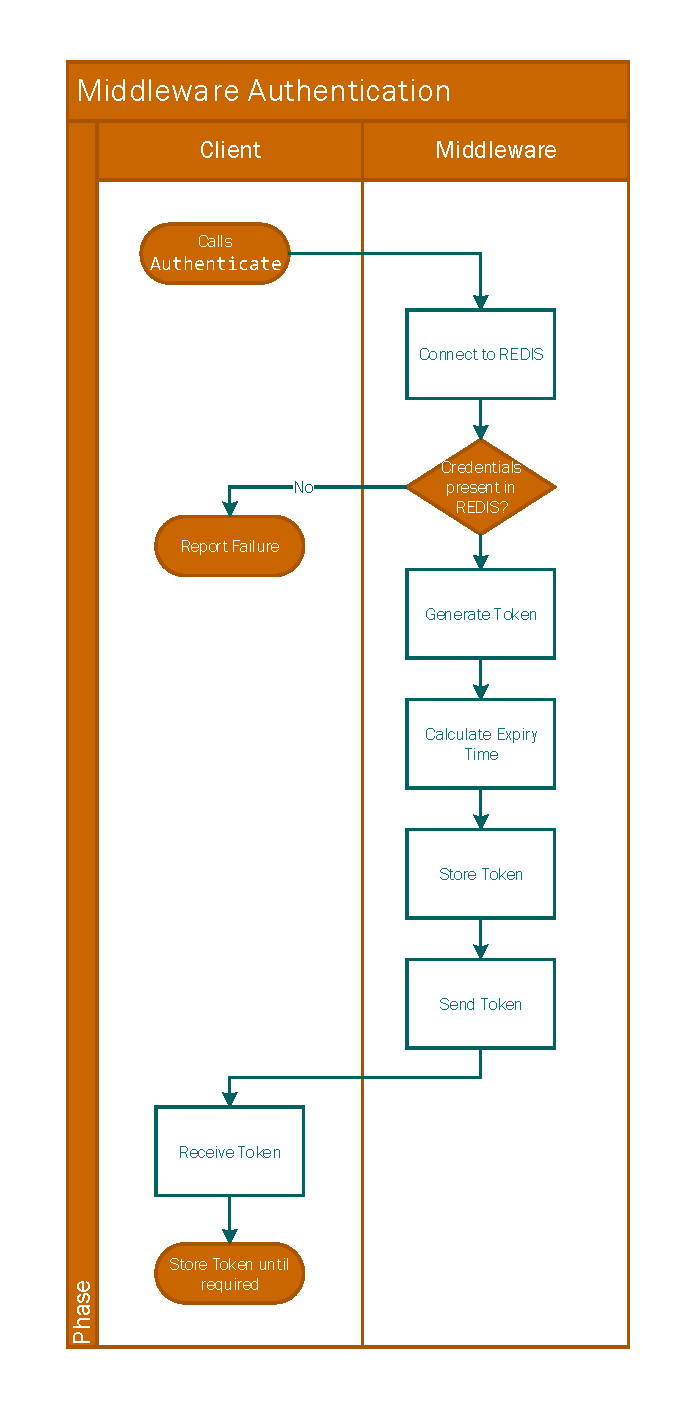
\includegraphics[width=\linewidth]{gfx/MiddlewareAurthentication}} 
\caption{Authentication work-flow}
\label{fig:aurth}
\end{figure}

Once the token has been received successfully the process shown in in \autoref{fig:aurthWithToke} is followed.

 \begin{figure}[!htbp]
\myfloatalign
{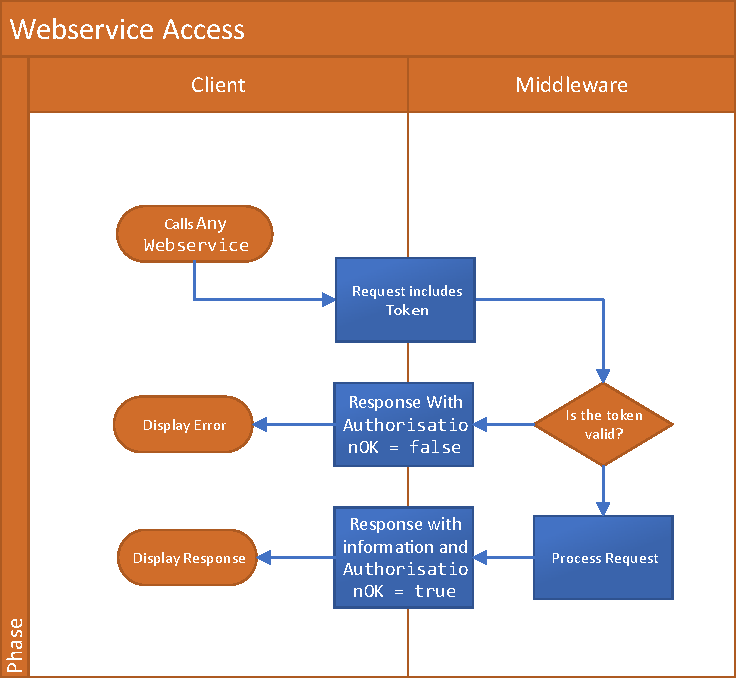
\includegraphics[width=\linewidth]{gfx/MiddlewareAurthenticationWithToken}} 
\caption{Use of authentication token}
\label{fig:aurthWithToke}
\end{figure}

Once the token has been issued to a client it is valid for a fixed amount of time (in the example implementation this is set at one hour, however this is defined as a constant for ease of alteration) after which the client receives an error if it is used. The client must then re-apply for a token, once again using the procedure set out in: \autoref{fig:aurth}. The use of tokens reduces the number of times an end users credentials must be transmitted securely over the network, which would otherwise need to be done with every call to the webservice. Aside from reduced bandwidth usage this scales better on the server-side; the token need simply be checked for validity, rather than recalling the users details and checking the stored password hash.

\section{Conclusions}

The case study in the following chapter made extensive use of this middleware and further conclusions are found at the end of that section.

In \autoref{ch:probstate} a number of questions are posed, first amongst them is:

\epigraph{\QuestionSecurity} 

The middleware is an example of a way to provide security to a datastore with none built in. REDIS, by design, has no security, leaving it to the consuming application for improved speed of data storage and retrieval, which is that project's main focus. When REDIS is hosted on a non publicly accessible server (or port) and accessed via the middleware only authorised users can store or retrieve data. The technique used in the middleware of issuing tokens valid for a limited time has become popular within the industry, though other techniques could also be successfully applied. 

\epigraph{\QuestionCombine}

Using the middleware as an example we have shown that it is possible to combine multiple data stores by using the same intermediary to connect to all the different datastores. Services run within that intermediary have access to all datastores and thus can perform operations which aggregate data. 

\epigraph{\QuestionChange}

The use of a cut-out or intermediary between client software and a datastore can safe guard the client application against changes to that datastore or its interfaces. The middleware provides an example of such an application.

\epigraph{\QuestionSkillz}

The middleware acts as an intermediary with a known and easily understood interface with external developers. This was used effectively as part of the work presented in \autoref{ch:COMPASS}, where it is assessed.


\section{Further work}

More complete integration of differing data stores is possible - currently there is no webservice to summarise high frequency data and insert the bulk data into another store. This would be easily achieved within the existing framework, however, none of the projects for which the middleware was used have required it, thus it has not been implemented. Before the software could be commercialised it would be necessary to subject it to analysis by penetration testers to find any vulnerabilities in the security mechanism.

\subsection{Scalability}

%************************************************
\chapter{Combined Alternative Positioning and Signalling System}\label{ch:COMPASS}
%************************************************
\section{Introduction}
In the financial year 2015/16 Network Rail spent £106,008,691.22 \footnote{This information is made available by Network Rail at \url{https://www.networkrail.co.uk/who-we-are/transparency-and-ethics/transparency/datasets/}. The relevant data is headed \say{Payments for disruption on the railway made under schedule 8} and further data is available for schedule 4, planned disruptions.} compensating operating companies for unplanned delays. Every week many tens of thousands of delay minutes accrue on the railway, and of these many thousands are attributed to signalling failures. The delay caused to passengers as a result of such failures degrades customer experience and contributes to negative public perceptions of the railway. The Combined Positioning Alternative Signalling System,(COMPASS), is a system to provide a degraded mode signalling system with the primary objective of reducing the impacts associated with failures of the main signalling system. Fringe benefits of such a system also include improved vehicle positioning relative to the existing track circuit based system, leading to improved passenger information and the potential for use as a low cost primary signalling system on lightly used lines. 

This project was carried out in conjunction with industrial partners, and thus it was important that the end result was a demonstrator that could become a commercially viable product. This enabled the investigation of those questions pertaining to the available skills within the industry, those related to the deployment of ontology based architectures on a large scale alongside providing a means of verifying the work done in \autoref{ch:middleware}.

\subsection{The commercial case for degraded mode signalling}
The involvement in this project of commercial partners demands that it have a business case, in this case the project was completed in response to a request from Network Rail in conjunction with the railway safety and standards board and Future Railway. 

According to Network Rail historic delay attribution data available in appendix \ref{app:delaydata}, signal failures are responsible for a significant proportion of the delays on the UK rail network. Delays from a single type of signalling failure (track circuit failures) contributed 103260 minutes (over 71 days) of aggregated delays over a single 28 day reporting period, and these represent the largest delay for which the infrastructure manager is responsible. The industry is keen to explore potential solutions to issues caused by signalling delays. Network Rail, upon whom the costs fall, are particularly keen, as stated in \citet{MagazineRailTechnology2015} 
\begin{quote}
    [Network Rail] believe the COMPASS solution can reduce delays by improving the current signalling system’s ability to recover from system failures more rapidly, as well as providing enhanced resilience to the network for the future. 
\end{quote}

\subsection{Objectives}
In the tender request the customer (Network Rail) gives the purpose of the system as: ``to automate the manual processes involved in Temporary Block Working''. Temporary block working is the current fall-back procedure whereby trains are allowed to pass through sections of track where the signalling has failed. Several consortia are creating products in response to this tender and it is possible that more than one will be selected. In the UK rail domain the Infrastructure owner merely specifies systems, they do not design or build systems themselves, however they will evaluate the system in accordance with the tender document. To add complexity in this case the desired specification requested by the infrastructure manager changed over the lifetime of the project, as did the personnel allocated to it. This is a common challenge in real projects and thus representative of projects within the UK rail domain. Notably the amount of automation expected was reduced and the requirements altered such that there must always be a man in the loop. Furthermore it was clarified that the system would at no time be an \say{Alternative Signalling System}, rather it was to provide \say{Degraded Mode Working} and would never be used outside of those circumstances. 

The COMPASS demonstrator aims to show how ontology can form the core of a fall-back signalling system, reducing the impact of signalling system failure, keeping trains moving even when the main system has failed. The proposed solution is agnostic to the failed signalling system - either a traditional national signalling system employing a fixed block system or a modern moving block system.

The demonstration scenario assumed new equipment could be placed in two physical locations: In Cab, and in the Rail Operating Centre (here on ROC - effectively a control centre or modern signal box). It should be noted that cost is also important, this system cannot cost as much as a main signalling system, as such certain compromises are required. Guidance from Network Rail suggests that points should not be remotely controlled, rather the lie of the points should be detected and trains only routed where that permits. This reduces the safety criticality of the software and thus the level of (expensive) certification required. In particular the infrastructure operator wished to avoid the need for SIL level 4 certification, as such it was also requested by Network Rail that the system not issue trains authority to move without manual intervention. It is expected that improved knowledge of train location will also make possible improved passenger information.

\subsection{Client Requirements}
\label{sec:client}
The requirements from the client were set out in a tender documents \citep{NetworkRailInfrastructureLtd2015} and modified verbally, they may be summarised as:
\begin{itemize}
    \item The replacement of temporary block working with a more efficient solution. Originally this was the automation of temporary block working, however in light of guidance from the infrastructure manager there will still be a manual element;
    \item The system shall be deployed in a limited number of predetermined areas, were signal failures risk the greatest impact. This also differs from the original specification, which required scalability up to providing a national train position database. The area need not be a plain line, but can and likely will have multiple entrance and exit signals. The area can be bi or uni directional.
    \item The accuracy of train location data and hence arrival times estimation should be better than is available from the existing track circuit based systems;
    \item \say{System shall be separate from the existing signalling system};
    \item Be resilient to cyber attack, physical vandalism and deliberate sabotage;
    \item \say{maintain, in memory, train location to a given time stamp for reference purposes} ;
    \item Ease of adding other datasources when they become available would be an advantage;
    \item \say{adopt a multi-layered solution for train location.} That is take train position information from multiple sources. 
\end{itemize}

In order as to achieve the above objectives, in particular, the adoption of a multi-layer train location solution and the improved location accuracy it is necessary to bring together data from multiple sources. Use of an ontology architecture would minimise the development effort required to accomplish this.

\section{System design and specification}
In response to the requirements set-out in \autoref{sec:client} and in conjunction with industrial partners, the demonstration scenarios described in \autoref{sec:Scenarios} were designed. These scenarios made it possible to demonstrate that the techniques selected will be capable of meeting the client's specification and produced a system which, if the client chooses to proceed, can be commercialised. 

\subsection{Demonstrated scenarios}
\label{sec:Scenarios}
Two demonstrations were performed, in response to two different operational scenarios: The first demonstrates normal operation; the ontology with supporting tools connects to and process data-feeds from the UK infrastructure owner, Network Rail; this could include providing improved customer information. The second demonstration focused on the degraded mode operation itself and showed how vehicles could transition to COMPASS signalling and pass through a failed area of control. More details are given in \autoref{sec:demotwo}.

\subsubsection[Normal Operation]{Normal Operation - Quiescent State \\ First Scenario}
In the first scenario the railway is assumed to be operating normally, with the system in what is referred to as a ``Quiescent State''. In COMPASS this is used to demonstrate the system  monitoring the locations of services already running over the network, ready for use as the \say{base state} when a failure occurs. The train location data used in this scenario came from the Network Rail open data feeds, which were used in conjunction with a static map of the network, provided by the industrial partner. These two diverse data sources provide good examples of typical industry data sources, that may need integration in a functioning industry wide system. 

In normal operation the demonstrator tracks the locations of all the trains in the network, allowing the provision of better customer information as well as maintaining a model of the running system in readiness for degraded mode operation. This demonstrates that should a signalling fault occur the system would be able to respond appropriately. Tracking of locations is illustrated by displaying those positions on a map, annotated with the headcodes of the trains being tracked. A proposed extension to this scenario calls for the display of metadata for the train - projected arrival time for example - along with the headcode. The use of ontology in this project also makes easier displaying such things as live updated possible connections, in light of the arrival time. 

The quiescent state demonstrator monitors vehicle movements across the entire British rail network, and as a result provides solid evidence of the ability of ontology based systems to scale to the data volumes and rates needed in a nationwide industry deployment.

\subsubsection[Degraded Mode]{Degraded Mode \\ Second Scenario}
Degraded mode occurs when the underlying signalling system is not operating as intended, regardless of reason, and signaller chooses to use the COMPASS system to manage the train through the area, known within this project as the \say{area of interest}. It is expected, though not required, that the area will be relatively small and when the end of the area is reached the train returns to the control of the primary signalling system. 


\subsection{System Architecture}
A system was designed to meet the client requirements, which was capable of performing the demonstrations outlined in \autoref{sec:Scenarios}. This required sub-systems from multiple suppliers and which would, in implementation, be split between the signalling control centre, known in the UK as a \say{Rail Operating Centre} and the cab of every train fitted with the technology. For demonstration purposes all systems were present in the same room and physically connected; radio telecommunications being beyond the scope of the demonstrations. The demonstration system adopted the architecture set out in \autoref{fig:fullsys}. 

\begin{figure}[H]
\myfloatalign
{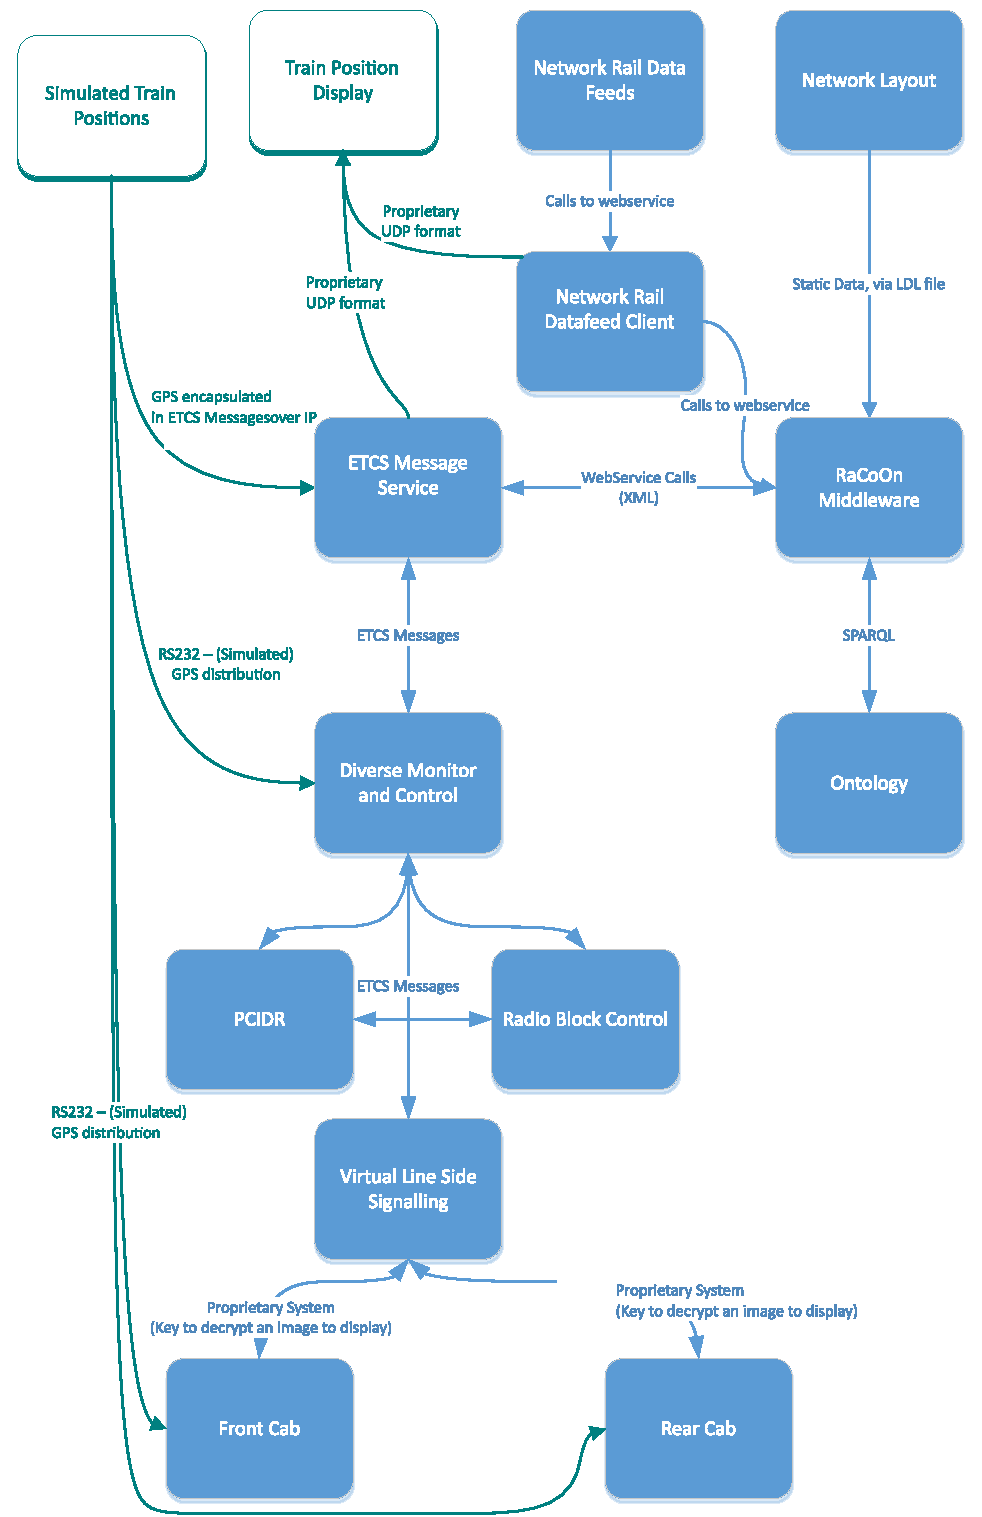
\includegraphics[max height=\textheight,max width=\linewidth]{gfx/FullSystem}} 
\caption{Full System Dataflows}
\label{fig:fullsys}
\end{figure}

The purpose of each sub-system is described in \autoref{sec:demoTwoOrg}. 

\subsubsection{Degraded Mode Demonstrator Organization}
\label{sec:demoTwoOrg}
The following elements are housed in the control centre:

\begin{description}
    \item[VLS Centre Comms] Virtual Line-side Signalling, which handles communications between the in cab elements and the control centre elements. This is a pre-existing commercial product modified for this project.
    \item[DMC - Diverse Monitor and Control] This component acts a central control block bringing all the other subsystems.
    \item[RBC - Radio Block Control] This is a standard part of a moving block signalling system.  It is a pre-existing commercial product which handles safety critical aspects of the system.
    \item[PCIDR] This `isolates' the points (switches). Whilst the system is in operation the points do not move. The current position of the points is detected and fed back to the rest of the system, which will only signal trains to pass in directions allowed by the points.
    \item[STiR Interlocking] This is a simplified version of a conventional signal interlocking, since the points are isolated.
    \item[RaCoOn] The Railway core ontologies. This integrates data from a number of different external and internal sources, alerting the other components when a train is approaching. This in turn comprises a number of sub-systems:
    \begin{itemize}
        \item The ETC Message service; This receives ETCS messages and triggers appropriate changes to the ontology;
        \item The RaCoOn Middleware, as discussed in \autoref{ch:middleware} it acts as a buffer between the others systems and the datastores;
        \item The datastores;
        \item A system to display train locations on a map. In this case an existing rail simulator, BRaVE which discussed further by \citet{Wen2015}.
    \end{itemize}

\end{description}

The data flows between these elements are illustrated in \autoref{fig:dataflow}. In order as to display instructions to the train driver (the system does not employ automatic train control at this point) a further in cab element is required. There are additional components used only for demonstration purposes, and would not have been included in the finished system.

\begin{figure}[H]
\myfloatalign
{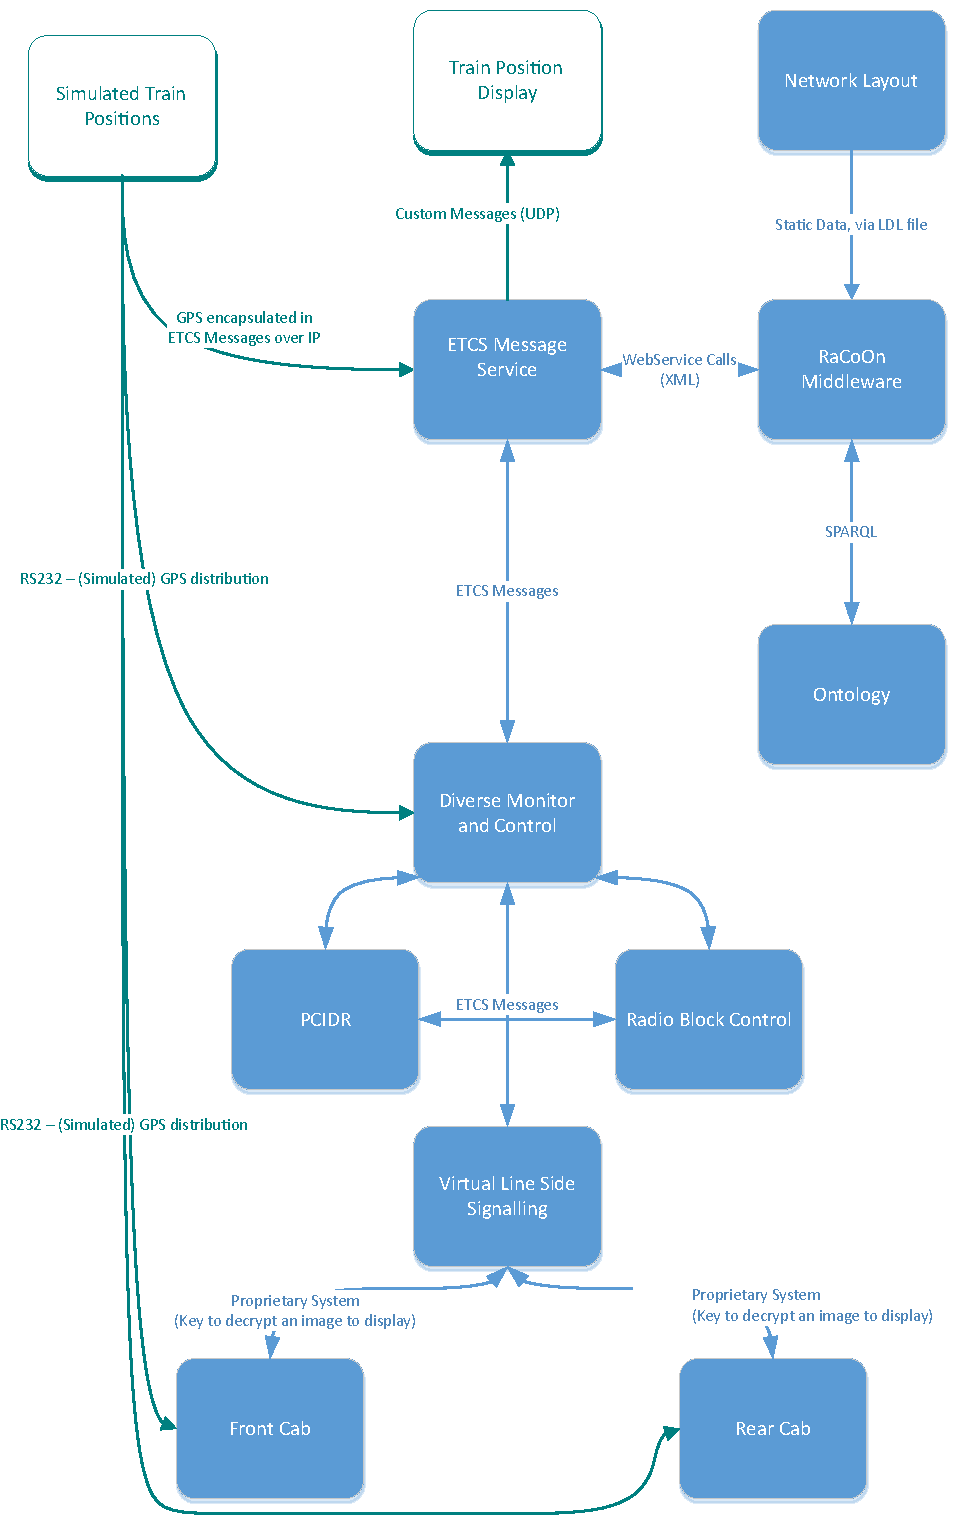
\includegraphics[max height=\textheight,max width=\linewidth]{gfx/Dataflow-StirDemoActive}} 
\caption{Demonstrator Two Dataflows. Note that links in green are demonstration only - not part of the final solution}
\label{fig:dataflow}
\end{figure}

As can be seen from \autoref{fig:dataflow} links between sub-systems, in particular those from different suppliers, use ETCS messages for communication. ETCS (discussed in \autoref{sec:etcs}) uses a standardised set of messages for communication with the train, and these messages are employed here between sub-systems. This was chosen for a number of reasons; firstly the industrial partners in this project had pre-existing expertise with this standard. Secondly the standard can easily be implemented over an Ethernet link, simplifying connection and lastly some sub-systems could only communicate in this manor. 

In order as to demonstrate the system it was necessary to use a rail simulator to recreate the effect of the train being in motion. The simulator generated coordinates representing the position of the front of the simulated train. These were sent to the in-cab signalling equipment in the same format as would have been used were the data coming from a real GPS receiver mounted on a train\footnote{A NMEA string delivered over a serial bus (RS232)}. The same position data was then sent to RaCoOn, to simulate the train sending position data. 


\section{Data Sources}

A number of specific data resources would be needed to support the demonstrators outlined in \autoref{sec:Scenarios}. These are detailed in the following sections and illustrated in \autoref{fig:AllSources}:

\begin{figure}[h]
\myfloatalign
{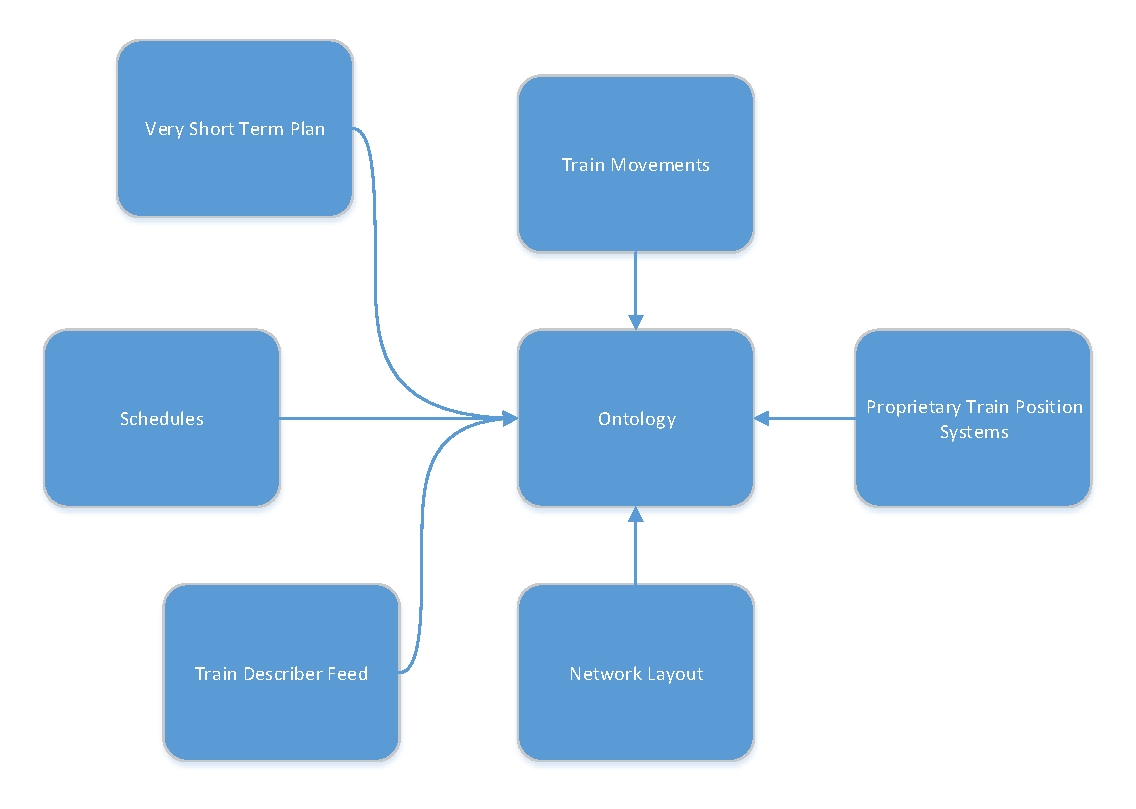
\includegraphics[width=\linewidth]{gfx/DataflowStirAllOptionsDemo}} 
\caption{All Possible Data Sources for integration}
\label{fig:AllSources}
\end{figure}


\subsubsection{Schedule Data}
For this project schedule data was obtained in the format of CIF files. This is a dense data format, holding weekly advance schedules.

Schedule data is comparatively coarse, primarily listing station calling times, alongside some supplementary information regarding the type of rolling stock used. In this file the trains are identified by headcode, which is unique on the rail network at any one time, however multiple trains are assigned the same headcode at different times. A further unique identifier is therefore supplied, which can be linked to other data feeds, but not directly the train describer feed, which uses only the headcode. This datasource is described in more depth in \autoref{sec:datatoimport}.

This is parsed using the tool described in \autoref{ch:cifparser}.
   
\subsubsection{Train movement data}
Train movement data, from the Network Rail webservices in particular the train describer feed. This feed supplies messages when a train steps from one signalling ``berth'' to the next.

Data is taken from the train describer feed, which is provided by Network Rail \footnote{available at: \url{stomp:tcp://datafeeds.networkrail.co.uk:61618}}. This feed provides messages from the train describer, which is a part of the signalling system that provides information to the signaller. This demonstrator uses only the ``Berth Step'' messages, which are generated whenever a train moves from one berth to the next. In the context of a signalling system berths are a region of track, protected by a signal, in which a train is located, a further definition may be found in \citet{Woolford2004}. As such the progress of a train across the network can be tracked, if used in conjunction with a map of signalling berths.

For this project it provided one of the key sources of train location data, obtained on a national level, to demonstrate the ability of the system as a whole and ontology in particular to process data on this scale.

\subsubsection{Absolute Position Data}
The absolute position of a rail vehicle, that is its position relative to the surface of the planet can be obtained from a Global Navigation Satellite System (GNSS), based on timing signals from satellites in known geostationary orbits. Positions are normally derived in terms of latitude, longitude and altitude which then needs combining with further data (typically a map) in order as to be meaningful to users. The Global Position System is the oldest and implementation of this and is the system chosen for this project, based on the low cost of compatible hardware. Were this project commercialised a full evaluation of the available options would be required.

Position can be expressed using multiple coordinate systems and projetions. The system chosen depends on the area that needs to be represented and how the data needs to be manipulated. A through review of map projections is well behind the scope of this thesis, however the following projections were used:
\begin{itemize}
    \item WSG84
    \item OSG36
\end{itemize}
WSG84 is the standard coordinate system used with GPS. It covers the entire globe, which it models as a spheroid. OSG36, commonly known as British National Grid is a coordinate system used only within Great Britain. It used only for display purposes in this project, since the available maps for displaying data used this format. 

It is intended that when this project is implemented GPS provides the more accurate data stream, allowing for better customer information and providing a fall-back in the case of failed track circuits, as well as making it possible to run trains closer together.

GPS data was simulated for the demonstrators. The data recreated a feed from a GPS unit fitted to a train cab and as such the data was supplied as a standard NMEA string, wrapped in an ETCS message. Accuracy issues were not considered in this demonstrator, had they been there would have been a need to combine balise pass data, to know which line a train was on, with the GPS data, since GPS accuracy is not always enough to know with certainty which of several parallel lines a train is on. The distribution of GPS data is further discussed and illustrated in: \autoref{sec:demoTwoOrg}.

For this project it was sent wrapped in standard ETCS messages, using packet 44, which is reserved for applications outside of normal ERTMS/ETCS operation.

    \subsubsection{Static network layout}
The static track layout information was provided in LDL format.

The network map is static data loaded once and not changed. This network map was obtained in layout description language (LDL) format. LDL Format is a proprietary standard used internally within Siemens to describe the rail network, including all the infrastructure positioned on the network. The information is stored in a human readable and editable form, though tools to edit and display it exist and were used in this project. LDL files list first the most basic infrastructure, track, which is described as a series of nodes and edges, then the positions of increasing complex elements are overlaid, using a node and offset location system. This ``Node - Edge'' way of modelling the rail network sits well with the ontology, which also represents the network as a series of nodes and edges, though these are not the same as the nodes and edges that constitute the ontology. \citet{Tutcher2015} sets out the rational behind the modelling.

    \subsubsection{Additional datasources}
Beyond the datasources listed above it would also be possible to use the following data sources, though they were not fully implemented in the demonstrators produced:
\begin{description}
    \item [Train Movements Feed] This is another open data feed provided by Network Rail;
    \item [VSTP - Very short term plan] This data feed gives details of trains scheduled at short notice;
    \item [Other signalling systems] In particular direct connection to the train describer system (not via the webservices) was suggested for the final implementation of this project;
    \item [GPS data from the rear of the train] This would make it possible to provide accurate train integrity information, as required if implementing ETCS.     
\end{description}

 \section{Role of Ontology}

In the compass demonstrators the primary role of the ontologies is as the basis for data integration across diverse datasources. There are many data sources for this system and it is one of this project's objectives to show that the project partners could work with data from a multitude of heterogeneous sources, not limited to those included in the initial design. 

Ontology is also used for classification in this project, for example for the classification of nodes, which are classified by sub-type. Nodes can be any of the many types of object located on the track such as: simple nodes, points nodes or signals. Most significantly they can be the signals that mark the start of the area of interest; this information is used to determine when to trigger degraded mode operation.

\section{Demonstrator Implementation}
In order as to provide the demonstrations outlined in \autoref{sec:Scenarios} a system was implemented, consisting of sub-systems from all the industrial partners. In moving to production the simulation would no longer be required whilst certification would be, however, the system is designed such that certification should be obtainable. 

\subsection{Demonstrator One}
\subsubsection{Overview}
 
The first demonstrator, that which sought to show the system under normal operation or within its ``Quiescent stated'', aims to show that using the Network Rail data feeds, it is possible to track the location of multiple trains on the network. Physically this is presented as a geographical map showing the train line on which the capability is being demonstrated with labels showing the current location of running trains. The map is presented in \autoref{fig:DemoOneBrave}. As the train steps to a new berth, so these labels move, with the same granularity as is provided by the signalling system. Running on a physically separate system (though this is not required from a performance perspective) a client written specifically for this task displays the messages in a human readable format, as shown in \autoref{fig:DemoOne}. The ontology holds position data for certain signals on the track in the area on which the system was being demonstrated, these are returned to the map via the tool. Where data is not available the ontology returns nothing and thus no message is sent to display system. In this case display is provided by the centre's own simulator, BRaVE, which was being used solely for display purposes.

\begin{sidewaysfigure}
\myfloatalign
{\includegraphics[width=\paperwidth]{gfx/DemoOneBRAVE}} 
\caption[Realtime Train Position via BRaVE]{Realtime Train Position via BRaVE \citep{Wen2015}}
\label{fig:DemoOneBrave}
\end{sidewaysfigure}

\begin{figure}[h]
\myfloatalign
{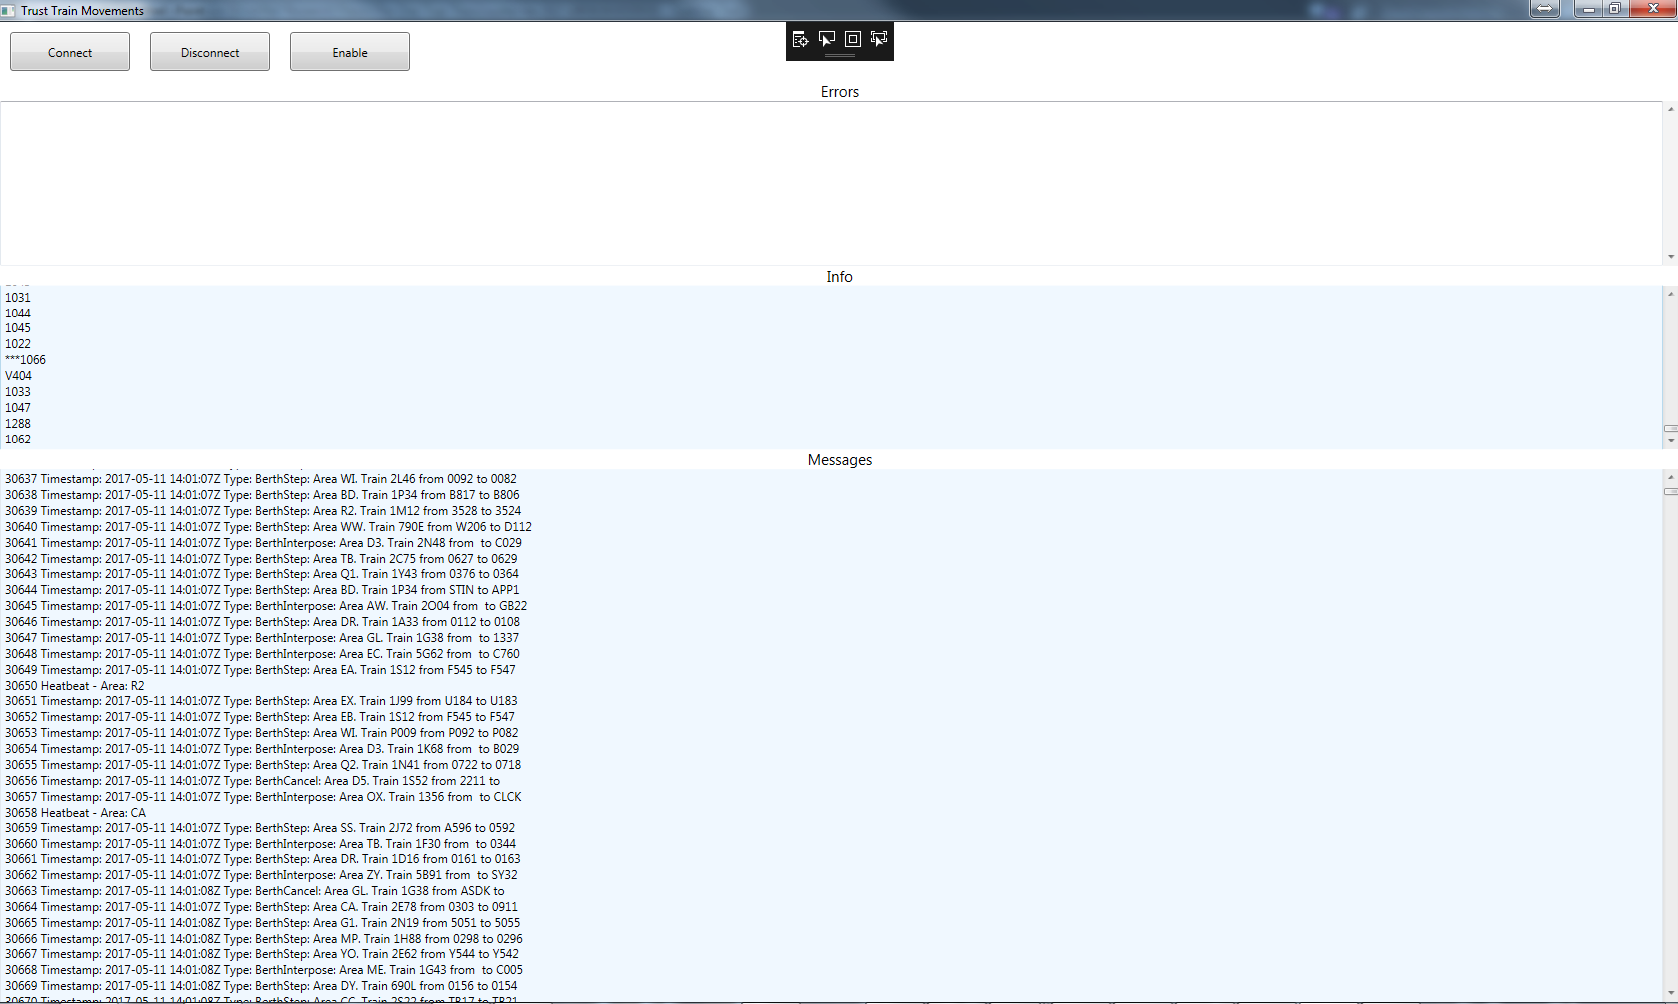
\includegraphics[width=\linewidth]{gfx/DemoOneScreenShot}} 
\caption[Demonstrator One]{The first Demonstrator in use}
\label{fig:DemoOne}
\end{figure}


\subsubsection{Model Changes}
This demonstrator made significant use of geographical data, \citet{Tutcher2015} gave a number of suggestions as to how geographic data be handled, in particular it recommended the use of the ``W3C Basic Geo Vocabulary''\footnote{\cite{Lieberman2007}}, alongside the RaCoOn \texttt{u:location} class. This recommendation was followed and geographical locations were encoded using that schema. 

Elements relating only to this project, all of which extended elements from the existing ontology, where placed in an application ontology design specifically for the COMPASS project, shared between both demonstrators. As per the guidelines set out in \autoref{ch:cifparser} this was the lowest level at which it was appropriate to model the concepts and avoided adding unnecessary complexity to those modules shared throughout the domain.

\subsubsection{Advantages of this approach}
The most widely discussed advantage of this approach, that is the use of ontology for data integration as opposed to constructing case by case integrations, is that of ease of adding further data sources without alteration to the existing system. The separation of business logic, which can be moved to the ontology, how one decides where the area of interest is for example in this case, also makes for more maintainable and resilient systems. 

\subsubsection{Implementation}
In the first demonstrator the ontology is used to match signal berths to their physical locations. A SPARQL query shown in \autoref{lst:selectsignallocation} is used with the signal's identifier to retrieve its location. This query is triggered by the arrival of a birth step message from the Network Rail train describer feed then, if found, the resulting latitude and longitude are first converted to British national grid coordinates, before being sent onwards to BRaVE for display. 

\begin{lstlisting}[float=h,language=sparql,frame=tb,caption={SPARQL to select a signal location from its identifier. Note some of the features here are Stardog specific, in particular the passing in of the @sigid parameter},label={lst:selectsignallocation}]
SELECT  ?lat ?long
WHERE {
    ?Signal a <http://purl.org/rail/core/Signal> .
    ?Signal dc:identifier ?ident   .
    FILTER( regex(?ident, @sigid )) .
    ?Signal core:relativePosition ?signalPos .
    ?signalPos u:measurementValue ?offsetVal .
    ?signalPos core:locatedOn ?track  .
    ?savedPos core:locatedOn ?track .
    ?savedPos a geo:Feature .
    ?savedPos wgspos:lat ?lat .
    ?savedPos wgspos:long ?long .   
    ?savedPos core:hasOffsetLocation ?savedOffset .
    ?savedOffset u:measurementValue ?savedOffsetVal .  
    FILTER(?savedOffsetVal = ?offsetVal)
}
\end{lstlisting}

\pagebreak

The data flows within this demonstrator are set out in \autoref{fig:DemoOne-DataFlow}, which shows that much of the system remains inactive in this scenario, as much of the system is dedicated to managing the train through areas of failed signalling.

\begin{figure}[H]
\myfloatalign
{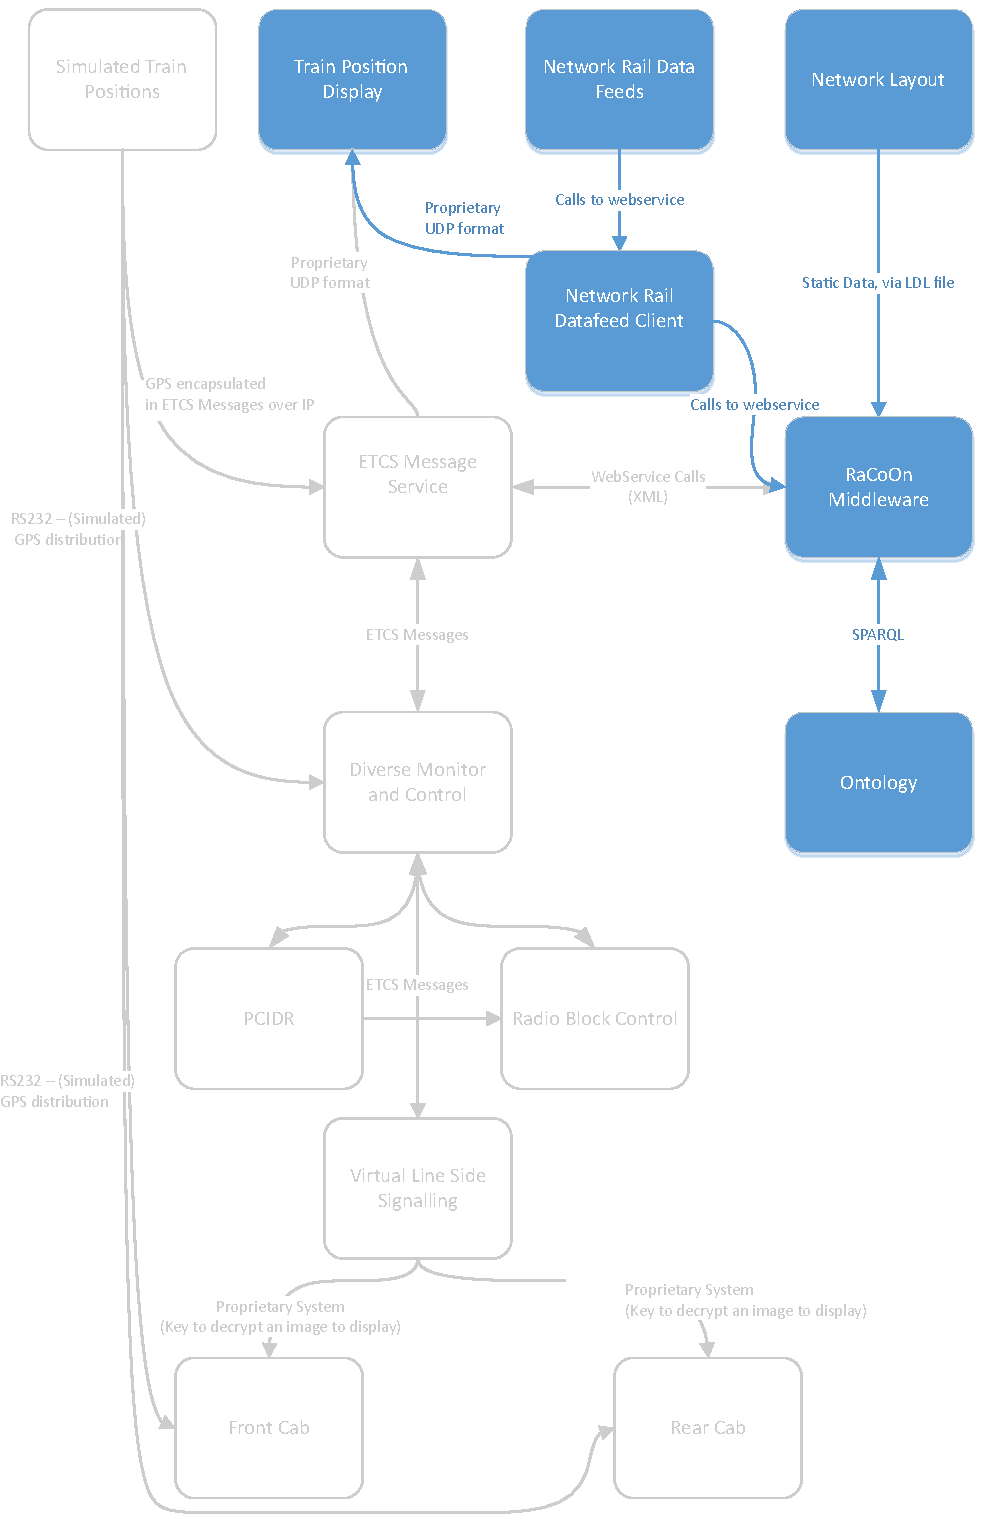
\includegraphics[max height=\textheight,max width=\linewidth]{gfx/Dataflow-StirPassiveDemo}} 
\caption[Demonstrator One Data-flows]{Demonstrator One Data-flows \\ Objects and data-flows shown in grey are connected but inactive}
\label{fig:DemoOne-DataFlow}
\end{figure}


A modular architecture was employed in both demonstrators to allow the reuse of components and to ensure separation between functionally distinct units. The first demonstrator comprised the following modules:

\begin{description}
    \item[MiddlewareConnectivity]
    This was compiled as a DLL and used in both the client to receive Berth Step messages from Network Rail, as used in the first demonstrator, and the tool for receiving ETCS messages used to demonstrate the second scenario. This module provided a range of functions for interacting with the RaCoOn middleware and thus the ontologies and REDIS. For reasons of development time some SPARQL   was embedded in this module rather than being encoded as rules in the ontology. Embedding SPARQL does mean that a certain amount of the process and decision making embedded in the software rather being abstracted to the ontology, however all of the classification remained within the ontology.    

    The middleware connectivity module handles the security process used by the middleware, holding the token and renewing it when it expires. For the purposes of demonstration the username and password were hard coded, though were this system deployed in a live environment they would be supplied by the user. A credential storage mechanism, is provided in readiness for moving over to that implementation. 

    A class is provided which lists the URI's used throughout the system as constants to avoid both ambiguity and the need to type URI's each time they are referenced. Whilst packages exist to auto create this for JAVA nothing was available and compatible with stardog via C\#. This class makes the URI's available both as strings and, where appropriate, as C\# URIs, so as to alleviate the need to constantly create new URIs, this is both more convenient and efficient. Other classes provide constants for other purposes:
    \begin{itemize}
        \item Locations of webservices
        \item ETCS Messages Numbers
    \end{itemize}

    The middleware connectivity module abstracts the ontology centric triples view of the world into C\# objects and handles the details of contacting the correct webservice. To this end two objects are provided: one representing a triple and another a node; these in turn hold methods for representing their contents as SPARQL, for the purposes of building queries. It was found, by experimentation, to be far quicker hold this representation of objects in memory then do the conversion to SPARQL and run the query via dotNETRDF than it was to use dotNETRDF's inbuilt graph to SPARQL engine. It was also found, again by experimentation, that since by design stardog performs reasoning whenever new data is inserted it is necessary to group records together and perform fewer large inserts rather than many small inserts. This too is handled in middleware connectivity. All data to be inserted in the triple store implements an interface, \texttt{IConvertToTriples}, following the C\# naming convention of naming interfaces with a capital `'I', which enables other functions to iterate through all data to be inserted, regardless of type. Parsing to and from XML data is also handled within this module.

    \item[TrustMovements]
    This module, compiled as Windows Presentation Foundation (here on WPF) application contains the logic specific to the first demonstrator, including the connection to the train describer webservice, which is implemented as a singleton. The rest of this module broadly follows the Model - View - View Model pattern, as is common practice with applications implemented in WPF. As you would expect with an MVVM application the GUI is defined in XAML with very little code behind. The train describer feed is provided using the ``STOMP'' protocol and the following stomp-client was used to access it: \url(https://github.com/openraildata/stomp-client-dotnet), which in turn uses the Apache NMS (.Net Message Service) \footnote{available from: \url{http://activemq.apache.org/nms/}}. The Apache NMS libraries were obtained using the .Net library management service, NuGet. 

    The view model class, as is normal in this architecture, formats the messages retrieved in order as to display them, presenting them to the view as properties and implementing the \texttt{INotifyPropertyChanged} interface to notify the view of new values. A controller class is used, slightly unusually for this architecture; this handles the threading and timing details, alongside checking with the ontology (via racoonmiddleware) if there is position data available for a given train movement. In this demonstrator one thread was used to connect to the webservices, a process which is subject to delay, another to obtain a position from the ontology (also subject to some delay) whilst the GUI was on another separate thread. 

    \item[BraveConnectivity] This was compiled as a DLL and because of the modular architecture employed it was possible to reuse this module in the ETCS Message Service, which was required for the second scenario.

    The module implements the singleton design pattern, to ensure only one connection with BRaVE will ever be made at any given point in time, in turn ensuring that resources are correctly freed when the system is shut-down and making it clear to others who use this module that only one instance will be required. This module has functions to convert WGS84 coordinates to those used in BRaVE; OSB36. Beyond this it also serializes the data to the format used by brave (XML) using an agreed specification. 

    
\end{description}

For data integration the existing Rail Core Ontology was used then another smaller application ontology was created to model the data used in this project. A mapping was made to the RaCoOn and thus it was possible to integrate data from other sources. One contribution this could make, though it was not fully implemented in the demonstrator, is the integration of schedule data, already available to the ontology, and train describer level train location data which was made available to the ontologies as part of this project. The decision not to implement was taken based on the complexity of matching routes across the network to information in the schedule and the limitations of the project time scale.

\subsubsection{Outcome of demonstration}
The system worked as expected and was demonstrated to the client, who indicated it would be possible to proceed to the next round of the tendering process.
Videos of the two demonstrators in operation are available from: \url{http://morrisdigital.co.uk/video/}.

When this system was demonstrated to the client this system operated for a period of ten minutes and displayed the location of three trains, each of which moved multiple times.

Aside from the commercial goals of the project partners this project also made it possible to investigate the use of ontology on a national scale; the Network Rail train describer feed sends a message for every single \say{Birth Step}, that is movement between signalling births of a train in the UK rail network, which at busy periods can easily reach hundreds of messages a minute. These messages each trigger a SPARQL query to ascertain whether they are within the area of interest being shown by the demonstrator. This was done successfully, including use of property chains, without placing any significant strain on the data store, which was hosted on a desktop PC.

\subsection{Demonstrator Two}
\label{sec:demotwo}
\subsubsection{overview}

The second demonstrator aimed to show that it was possible to detect an approaching train and signal it through an area in which the main signalling system was not functioning. For this demonstrator it was not possible, for reasons of both cost and safety, to use the live railway, instead a simulator was used, in this case RETS (a train simulator used by the project's commercial partner). A part of the UK rail infrastructure was simulated, since an accurate (and verified, though outside of this project) model of that infrastructure was available, which was required.

Three scenarios were demonstrated.  
 \begin{itemize}
\item First a train moves across the simulator network area under normal signalling. Its progress is displayed on the a map. This demonstrates that the system can communicate internally, from the simulator to the ontology then onto the display. It further shows that the system can track the approaching train. This is shown in \autoref{fig:DemoTwo_S1}.
\item In the next scenario the train drives into an area, then the signalling fails and the alternative system, known as STiR is activated. The driver is instructed, via the in cab signalling, to drive out of the area of failed signalling then to obey normal signalling once the train is clear. This is shown in \autoref{fig:DemoTwo_S2}.
\item In the final scenario an area of signal has failed, a train approaches, is switched to STiR control and leaves. This is repeated with a second train. This is shown in \autoref{fig:DemoTwo_S3}.
\end{itemize}

\begin{figure}[H]
\myfloatalign
{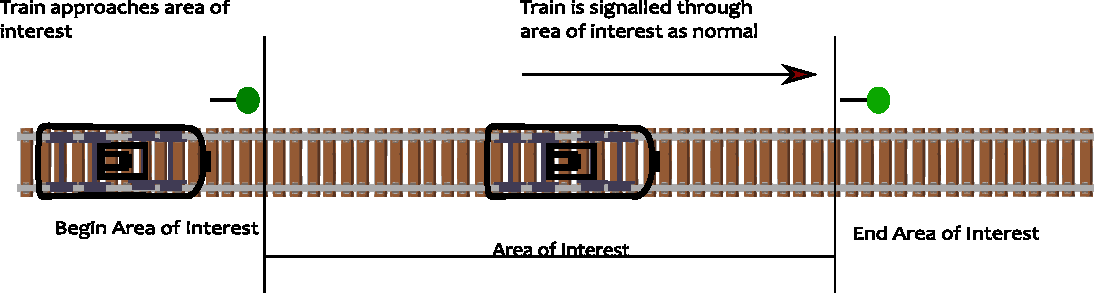
\includegraphics[max height=\textheight,max width=\linewidth]{gfx/DemoTwo_StageOne}} 
\caption{Demonstrator Two - Stage One}
\label{fig:DemoTwo_S1}
\end{figure}

\begin{figure}[H]
\myfloatalign
{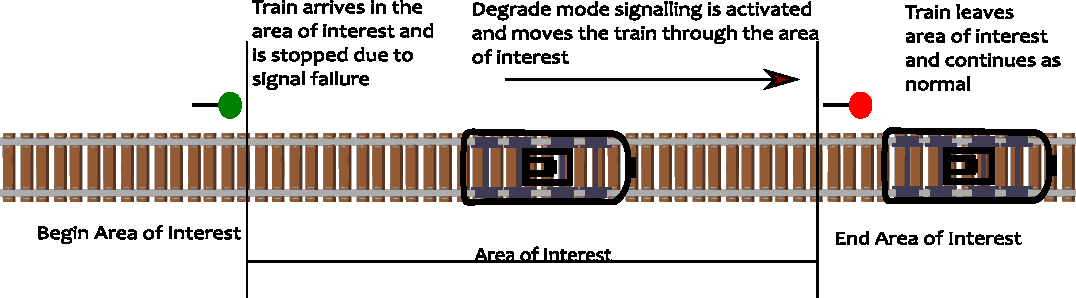
\includegraphics[max height=\textheight,max width=\linewidth]{gfx/DemoTwo_StageTwo}} 
\caption{Demonstrator Two - Stage Two}
\label{fig:DemoTwo_S2}
\end{figure}

\begin{figure}[H]
\myfloatalign
{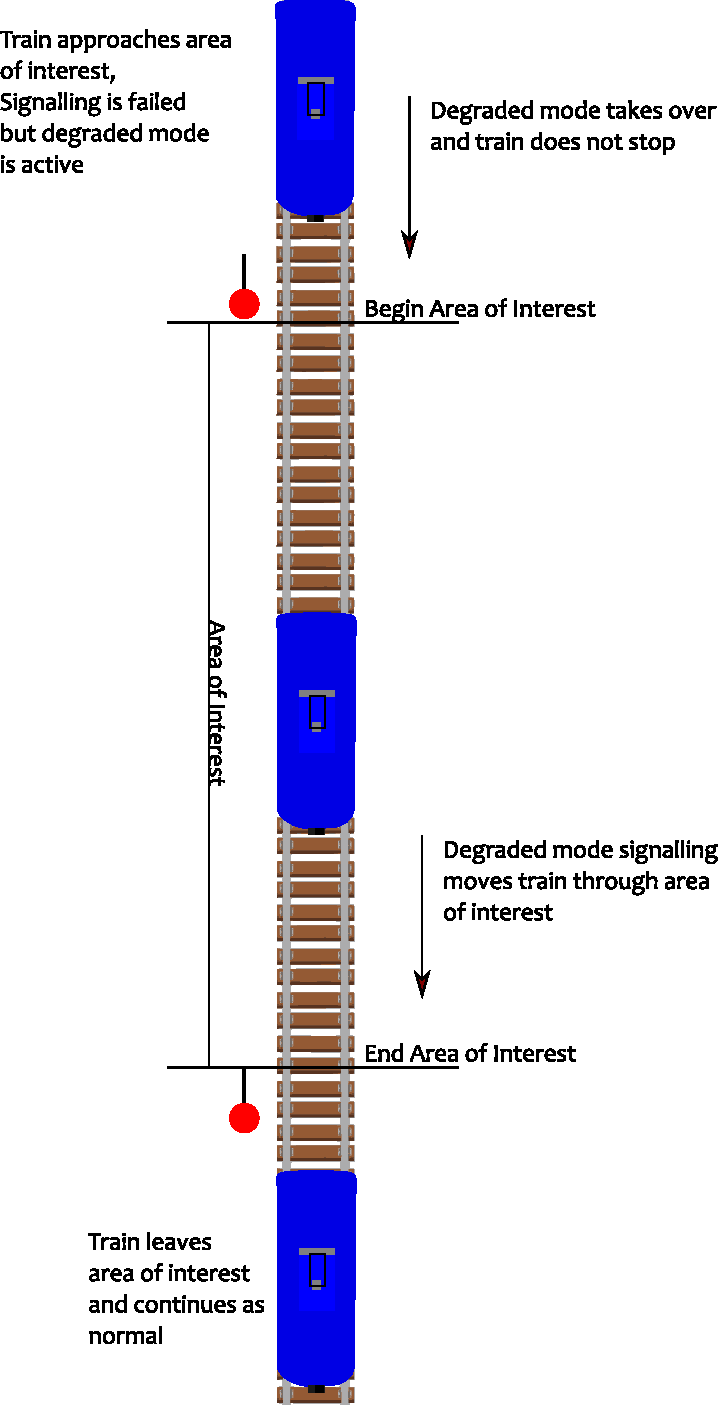
\includegraphics[max height=\textheight,max width=\linewidth]{gfx/DemoTwo_StageThree}} 
\caption{Demonstrator Two - Stage Three}
\label{fig:DemoTwo_S3}
\end{figure}

\subsubsection{Communications Implementation}

The layout of the RS232 bus is illustrated in \autoref{fig:RS232}, which is used only to disseminate GPS. Whilst for the demonstrator the front and rear cabs were connected via RS232 in reality this would not be possible, however, it is envisaged that when implemented the system would use a GPS receiver in each cab, which would output its position via RS232. The simulator would not then be needed, the GPS from the train would be sent via radio link to the VLS track-side component and from that via ETCS messages over IP on to the operations centre. 

All Subsystems also communicated over via Ethernet, either via the local loopback interface when multiple subsystems where hosted on the same machine or via a gigabit Ethernet switch. 

\begin{figure}[h]
\myfloatalign
{
\includegraphics[width=\linewidth]{gfx/RS232Bus}} 
\caption[Demonstator Two - RS232 Bus]{RS232 Bus. \\ Note that RETS is the train simulator which is the only transmitter on the bus.}
\label{fig:RS232}
\end{figure}

\subsubsection{Demonstrator Outcomes}
The second demonstrator, as with the first, performed flawlessly upon the clients inspection. This demonstrator also helped investigate the effect upon development time of middleware between the ontology and the client. In particular it made it possible to observe the effect of centralising functionality in the middleware and the extent to which ontology specialists would be required in such a project. 

A service was required to get from data sent as an ETCS message to insertion in the ontology, as it would be for most new formats when they are first encountered. This service acted a `Translator' between ETCS messages and the ontology middleware, which executed appropriate queries in response to any given message. For technical reasons integrating this functionally into the middleware would be challenging, however, from a performance perspective this architecture makes it possible to host the different components on different systems if required. 

\section{Conclusions}

\subsection{Benefits of Ontology}
The ontology and the surrounding tools allowed for significant decrease in the amount of time taken to integrate the various datasources required by the project into a coherent system. 

An interview was conducted with a senior engineer from one of the industrial partners, namely Lucas Redding from Siemens. In that interview Lucas stated that it would require significantly more time and expense to develop the system without the ontology than it did with. Furthermore it would have been necessary to decide at the outset of the project which data sources to use and contract external experts to integrate them with the system, since those skills were not available in house. Whilst it is the case that is necessary to write adapters to new data-sources for inserting data to the ontology it was agreed, again by Lucas Redding, that significantly less development effort would be required. Had further data sources become available after the initial design it would not have been possible to add them with out significant redevelopment. This interview further illustrated the shortage of skilled personnel within the rail domain, proving the need for solutions to help the rail domain transition to ontology with few skilled personnel. 

Another key advantage of using the ontology on this project was that data previously made available to the ontology could be reused. Mapping schedule data to the ontology had already been partially completed, so it was possible to simply complete the mapping and use the existing work. Had this been done to a proprietary format that work would almost certainly have been of no value to this or other future projects. Going forward the mapping from the train describer feed will be available for use in other projects, as will the schedule mapping.

The existing RaCoOn ontologies provided a model of the domain, what would be referred to a ``Global Schema'' by \citet{Lenzerini2002}. A mapping was made between the data sources and RaCoOn, which resided in a separate ontology and file. This is available via github.

\subsection{Role of tools to connect to the ontology}
 
As with data, re-usability was also seen with tools, such as the middleware, which made connection to the ontologies and the triplestore that hosts them possible. Without the middleware it would have been necessary to handle the connection to the datastores as part of this project, which would have added significant development time. The same is true of the tool to parse the schedules in CIF format, discussed in \autoref{ch:cifparser}, had that tool not been available it would have been necessary to create such a tool from scratch, significantly impacting the projects time line.  

Without the middleware it would have been necessary to implement much of the functionality contained in the middleware, in particular that relating to querying the datastore. The project would then be tied to using the chosen datastore and unable to change as new the industry developed.

\subsection{Questions Answered}

This project allowed us to address the following questions:
\begin{samepage}
\subsubsection*{\textit{\QuestionOtherData}} 
This project illustrated both how diverse the data environment can be in the rail domain and how this presents a barrier to improved performance. \end{samepage}The datasources are largely in historic formats, devised when a system was commissioned and where necessary encapsulated in a more modern protocol. These encode in them a great deal of knowledge as to how individual systems operate; for example the ``Birth Step'' messages used in this project require an understanding not just of railways in general, but signalling systems in particular in order as to make them useful. This presents a problem using them with systems that view the world differently; perhaps as maps which are interested in absolute position, for people using modes of transport other than the railway in order as to get to a station as opposed to the network position view of signalling systems. Another problem is that of the skill set required to work with the data, a developer primarily experienced in creating usable mobile phone applications would struggle to interpret the data correctly.

\begin{samepage}
\subsubsection*{\textit{\QuestionSkillz}} 
The middleware was used in this project, in part, to reduce the amount of development time required, since this project was conducted with only one ontology engineer and a condensed time-line. The functionality already existing in the middleware was beneficial, however, it was found that the project still required significant development effort from an engineer with knowledge of ontologies and software development; multiple man-months were required for the development of the various systems connected. Further development of the middleware will reduce this, however, this project provides no evidence that it would be possible to connect external data sources to the ontology with no ontology engineering experience. 

The functionality within the middleware to handle connections to the triplestore and act as an interface however alleviated the need to develop this functionality specifically for this project. Where it was necessary to extend the middleware those extensions in turn will be beneficial to future projects. 
\end{samepage}
It was discovered that the commercial partners do not have expertise in this area, emphasising the need to provide solutions which do not require large numbers of skilled engineers. The engineers from the commercial partners all had very extensive experience of software development (and all specialised in signalling systems) but as was stated by Lucas Redding when interviewed they did not have ontology experience within the company. 

Beyond the question of interfacing with the ontology there is that of extending the model. This project required the creation of a small application ontology holding data pertinent only to this project, not the broader signalling nor rail domains. That required an engineer with knowledge of ontology modelling, though in this case the development time was far more limited; the concepts to model were much simpler and most were already modelled in the ontology. As with connecting the software to the ontology however, some extra development will be required for most projects.

\begin{samepage}
\subsubsection*{\textit{\QuestionChange}} 
The information systems in this project are now independent of the datastore's interface, were the datastore to change the interface it presents that would require only a change to the middleware, as discussed in \autoref{ch:middleware}.
\end{samepage}

This project served to highlight another unforeseen issue in terms of protecting projects from a complete change of triple store, namely that of differing feature sets.\say{GEO-SPARQL} was required in order as to ascertain the distance between points and this is not supported by all triple stores. As such, even with the middleware as an intermediary, it would still only be possible to swap Stardog for another triple store which offered that support, without significant development effort. 

\begin{samepage}
\subsubsection*{\textit{\QuestionCanOntologyScale}}
The first demonstrator successfully handled signalling data at national scale. Data from conventional (fixed block) signalling systems is, by the standards of modern computing, not truly high velocity and could as such be handled by the triple store alone, with out needing to resort key value stores.
\end{samepage}


\section{Further Work}
It would be beneficial to move functionally embedded in C\# code to the ontology. In particular a number of rules and queries which were for reasons of development time hard-coded should have been represented as rules processed by the triple store. This would remove the dependency on software engineers for editing that logic.
%************************************************
\chapter{Conclusions}\label{ch:Conclusions}
%************************************************
The information environment within the rail industry is very diverse, with a range of heterogeneous systems of differing ages and significant scope for improved integration. The literature review (\autoref{ch:litreview}) identified the benefits available to many stakeholders from improved data integration, such as reduced costs thanks to the removal of barriers to data integration. 

The COMPASS project, discussed in \autoref{ch:COMPASS}, showed that one of the barriers was a shortage of software engineers with ontology engineering experience and showed one way in which that barrier could be overcome. Another barrier identified was the integration of data sources available in one the proprietary formats typical of the rail domain; the schedule parsing tool, discussed in Chapter 4, demonstrated the feasibility of making such data available in a linked format suitable for integration. The schedule parsing tool, alongside the middleware considered in \autoref{ch:middleware} was reused as part of the COMPASS project demonstrating how ontology can serve to unlock value for many projects across the industry.

This chapter will now examine the questions identified in the problem statement (\autoref{ch:probstate}).

\section{Response to Research Questions}

\begin{itemize}
	\item \QuestionOtherData
	\item \QuestionSkillz 	
	\item \QuestionCombine
	\item \QuestionChange
	\item \QuestionCanOntologyScale
	\item \QuestionSecurity		
\end{itemize}

Considering each of these questions in turn:

\subsection{\QuestionOtherData}
Excluding data held in relational databases, many railway datasources are held in proprietary formats, often structured based not on the data they represent, but on the system which generated them. As was shown by the reuse of data from the schedule parsing tool in the COMPASS project, ontology provides a method of integrating data across different systems, constructed by different suppliers for different purposes. Even where two systems operate very differently it is possible to map data from both to a single ontology and thus the data may then be used by either; for example signalling systems are primarily concerned with passenger safety, whilst journey planning applications need to know how the railway can help transport a person from one place to another at a given time and have no interest in other details.

In \autoref{ch:cifparser} the processing of static data is considered, taking as an example schedule data which is updated on a weekly basis. The construction of a tool which takes the flat datafile containing the schedules and makes this available as RDF, which could then be inserted in the ontology, allows for the reuse of schedules in any project which uses ontology as a datasource. Another project COMPASS, reported in \autoref{ch:COMPASS}, could use imported schedule data in conjunction with other data sources to build a picture of train movements helps demonstrate the utility of ontology as a means of data integration. 

Developing custom tools to process data requires more development time, and hence expense, than using commercial off the shelf software, where it is available, however, much data in the rail industry is held in proprietary formats for which no processing tools are available. Taking proprietary datasources and making them available in a linked format requires both some understanding of the data sources and of the linked format in which it is to be made available; as such this task requires software engineers with, at the very least, some understanding of the rail domain and of ontology.

In summary it is possible to make typical railway datasources available to the ontology and this enables improved data integration.

\subsection{\QuestionSkillz}
This project showed that whilst it is possible to reduce the amount of input required from ontology designers and software engineers with ontology engineering experience, however there is no evidence that it is possible to remove that input entirely. A service logically situated between the triple store and the client application can reduce the amount of development time needed to add new interfaces or datasources to the ontology, by allowing software engineers to interact with familiar webservices and alleviating the need to learn ontology specific technologies, such as SPARQL. Where the middleware offers all the services required to interface with a given system, it should be possible to add that interface without any knowledge of ontology technologies. In this project it was however found that the systems requiring integration were of sufficient complexity as to require extension of the middleware and knowledge of ontology techniques to achieve integration. If the middleware layer had more functionality, and if the same middleware was used for multiple projects, then each progressive project would need less and less intervention from software engineers with ontology engineering experience. 

The tool presented in \autoref{sec:manualtool} presents a way of allowing unskilled users to add items to the ontology. This tool is useful for making small alterations, where the data has been modelled previously. 

\subsection{\QuestionCombine}
The implementation of a middleware layer, discussed in \autoref{ch:middleware}, demonstrates one way multiple data stores of different types can be combined. One central point, the middleware, has connections to two different datastores (easily and indefinitely expansible to any number of datastores) and potentially any number of clients. Webservices included in the middleware have access to all the connected data stores; there for it would possible to implement a single webservice which either summarised data in one datastore and stored the full data in another, or which stored only the most recent value in one store and historic data in another. Were data of too high a volume or velocity for ontology storage encountered it would be possible to use either of these techniques to allow as much reasoning as possible, whilst retaining fine grained data for more detailed analysis. 

\subsection{\QuestionChange}
An intermediary layer between the triple store and client applications can isolate client applications from change, with one caveat: if features specific to a given triple store are used then only other stores supporting that same feature may be used. This was demonstrated in \autoref{ch:COMPASS} where the addition of GEO-SPARQL tied that project to triple stores with that feature.

\subsection{\QuestionCanOntologyScale}
National scale data from the UK rail industry was used both to test the schedule import tool described in \autoref{ch:cifparser} and to demonstrate the capabilities of the COMPASS system discussed in \autoref{ch:COMPASS}. In the first case, the volume of data that needed to be processed presented a challenge which required significant optimisation; when that optimisation was carried out, it was possible to process the schedule data in a reasonable time period and make it available to the ontology. 

In the second case, the COMPASS system used data from conventional (fixed block) signalling systems to show train locations. This data was provided for the entire country, but, by the standards of modern computing, this data is not very high velocity and could as such be handled by the triple store alone. A query was performed each time a train movement was detected including, when a location was found to be in the triplestore, a geographical lookup and the system still performed well.

\subsection{\QuestionSecurity}
The imposition of a secure middleware layer between unsecured datastores and the wider network can add security to those data stores which lack it and simply the management of those that have it. An additional benefit of the middleware implemented as part of this project is that it provides a single-sign on that can be used to access all datastores, simplifying the credential management.




\cleardoublepage
\ctparttext{Supplementary Data}
%\addtocontents{toc}{\protect\clearpage} % <--- just debug stuff, ignore
%\include{multiToC} % <--- just debug stuff, ignore for your documents
% ********************************************************************
% Backmatter
%*******************************************************
\appendix
%\renewcommand{\thechapter}{\alph{chapter}}
\cleardoublepage
\part{Appendix}

%********************************************************************
% Appendix
%*******************************************************
% If problems with the headers: get headings in appendix etc. right
%\markboth{\spacedlowsmallcaps{Appendix}}{\spacedlowsmallcaps{Appendix}}
\chapter{Appendix A Manual Data Entry Tool GUI}
\label{app:mantoolgui}

The GUI used by the manual data entry tool.

As shown by \autoref{fig:mtLogin} the user is first required to log on. Note that for ease of use all details, except passwords, are stored on the client machine, using cookies.
 \begin{figure}[H]
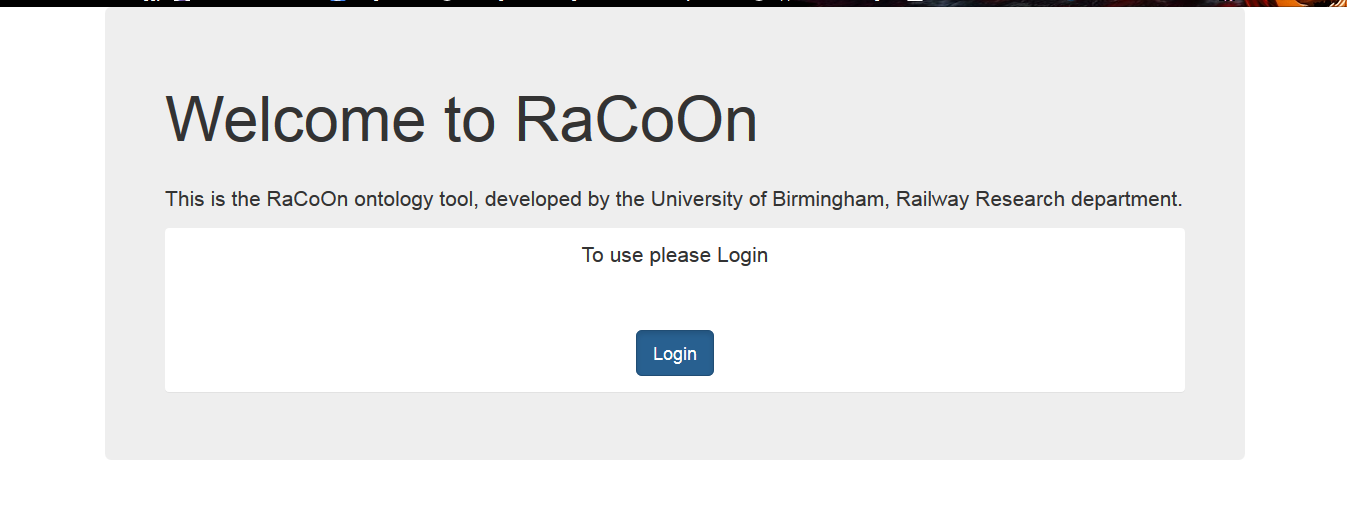
\includegraphics[max height=\textheight,max width=\linewidth]{gfx/manToolWelcome}
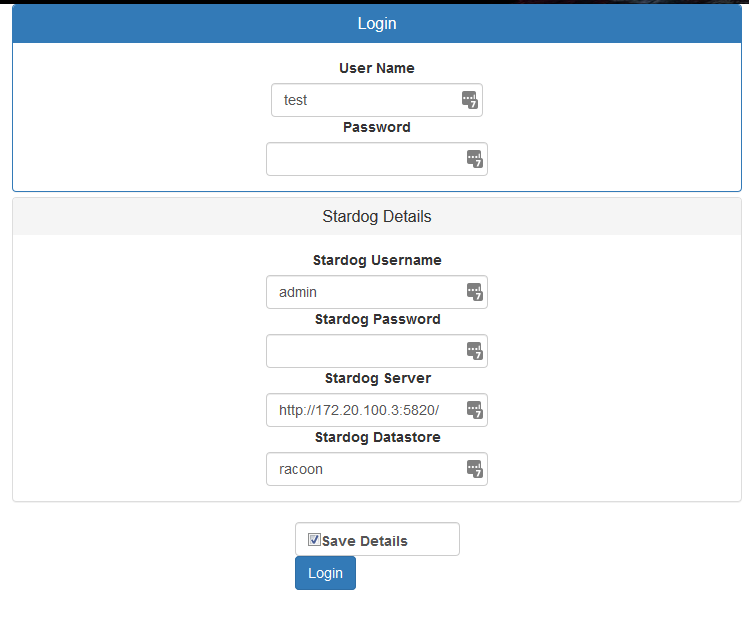
\includegraphics[max height=0.5\textheight,max width=\linewidth]{gfx/manToolLogin}
\caption{Manual Data Entry tool welcome and login screens}
\label{fig:mtLogin}
\end{figure}

If log-in is successful the user is presented with the main menu, as shown in \autoref{fig:mtMainMenu}. 
 \begin{figure}[!h]
\myfloatalign
{
\includegraphics[max height=0.5\textheight,max width=\linewidth]{gfx/manToolInUse}} 
\caption[Manual Data Entry Tool]{Manual Data Entry Tool main menu}
\label{fig:mtMainMenu}
\end{figure}

\section{Add an item}

 \begin{figure}[!h]
\myfloatalign
{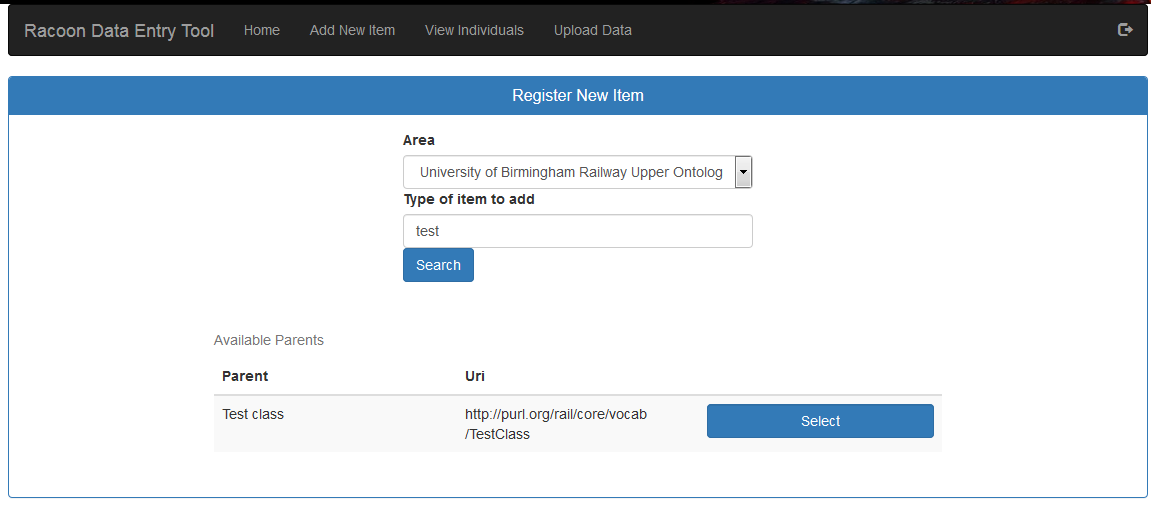
\includegraphics[max height=0.5\textheight,max width=\linewidth]{gfx/manToolAddingItem}} 
\caption[Manual Data Entry Tool Add item stage 1]{Manual Data Entry tool Adding an item stage one}
\label{fig:mtAddingItem}
\end{figure}

 \begin{figure}[!h]
\myfloatalign
{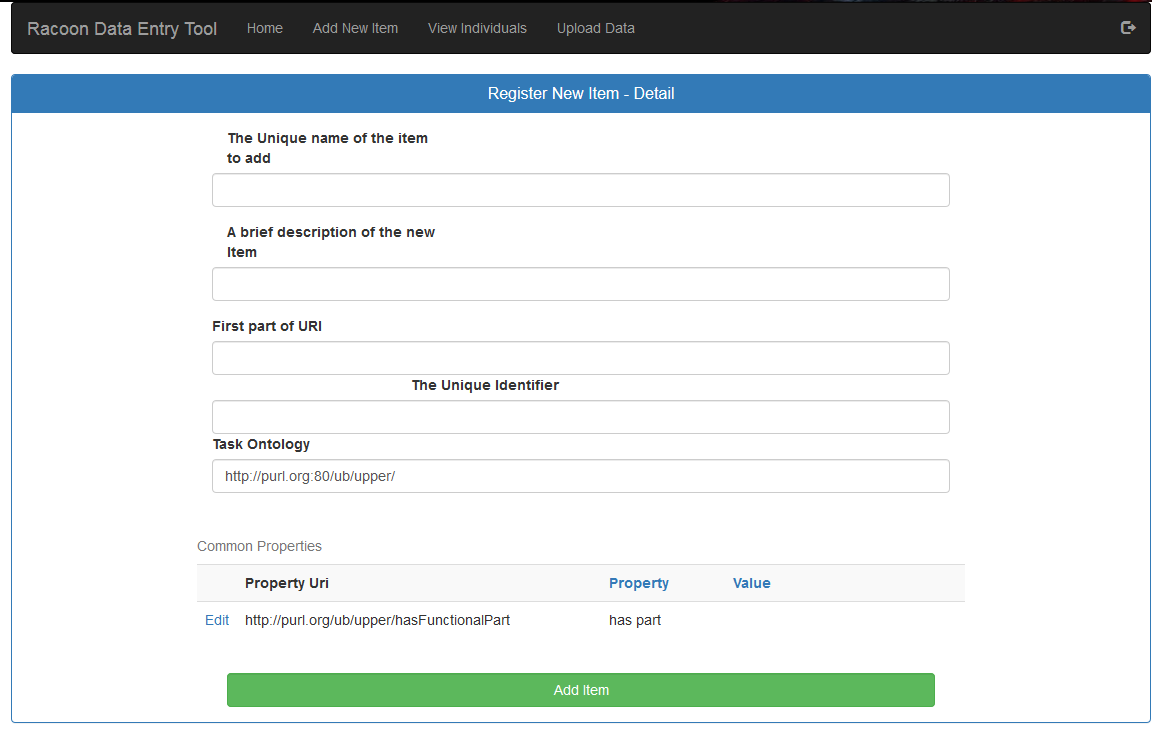
\includegraphics[max height=0.5\textheight,max width=\linewidth]{gfx/addItemDetail}} 
\caption[Manual Data Entry Tool Add item stage 2]{Manual Data Entry tool Adding an item stage two}
\label{fig:mtAddingItemDetail}
\end{figure}


\chapter{Stored procedure}
\label{app:spList}

The below provides an abridged listing of the stored procedure implementation used in the middleware.

\begin{lstlisting}[language={[Sharp]C},frame=tb,caption={The StoredProcedure class. Constructors, private fields and utility methods have been omitted for brevity.},label=lst:StoredProcedure]
 public class StoredProcedure
    {              
        private void createQuery()
        {
            lock (theQueryLock)
            {                
                //Cause the exception to be thrown here if the type doesn't exist, for clarity sake.
                Type queryType = Type.GetType(TypeOfQuerry, true);
                TheQuerry = Activator.CreateInstance(queryType) as IQuerry;
                if (TheQuerry == null)
                    throw new InvalidOperationException("The Query is not of a valid type");
                TheQuerry.SetTarget(Server, DataStore);
                TheQuerry.SetQuerry(StoredProcText);
            }
        }

        /// <summary>
        /// A hash of the storedproc name, used as a key to retrieve it
        /// </summary>
        public int KeyHash;

        /// <summary>
        /// The executable version of the query
        /// </summary>
        [XmlIgnore]
        public IQuerry TheQuerry
        {
            get
            {
                if (theQuery == null) createQuery();
                return theQuery;
            }
            private set
            {
                theQuery = value;
            }
        }

        /// <summary>
        /// The server at which the stored proc is targeted. Where this is null or empty the value from the Session is used
        /// </summary>
        public string Server;
        /// <summary>
        /// The Datastore at which the stored proc is targeted. Where this is null or empty the value from the Session is used
        /// </summary>
        public string DataStore;
        /// <summary>
        /// The name of stored proc
        /// </summary>
        public string Name;
        /// <summary>
        /// This is the name of the type of query to instantiate 
        /// </summary>
        public string TypeOfQuerry;
        /// <summary>
        /// The text of the command e.g. SELECT * WHERE {?s ?p ?o}
        /// </summary>
        public string StoredProcText;
    }
\end{lstlisting}
% 
%********************************************************************
% Appendix
%*******************************************************
% If problems with the headers: get headings in appendix etc. right
%\markboth{\spacedlowsmallcaps{Appendix}}{\spacedlowsmallcaps{Appendix}}
\chapter{Appendix  - CIF file parser log}
\label{app:ciflog}


 % was a completely unncessary log file, including as summary in relevant chapter instead

%********************************************************************
% Other Stuff in the Back
%*******************************************************
\cleardoublepage%********************************************************************
% Bibliography
%*******************************************************
% work-around to have small caps also here in the headline
\manualmark
\markboth{\spacedlowsmallcaps{\bibname}}{\spacedlowsmallcaps{\bibname}} % work-around to have small caps also
%\phantomsection 
\refstepcounter{dummy}
\addtocontents{toc}{\protect\vspace{\beforebibskip}} % to have the bib a bit from the rest in the toc
\addcontentsline{toc}{chapter}{\tocEntry{\bibname}}
\label{app:bibliography}
\printbibliography

%\cleardoublepage%*******************************************************
% Declaration
%*******************************************************
\refstepcounter{dummy}
\pdfbookmark[0]{Declaration}{declaration}
\chapter*{Declaration}
\thispagestyle{empty}
Put your declaration here.
\bigskip
 
\noindent\textit{\myLocation, \myTime}

\smallskip

\begin{flushright}
    \begin{tabular}{m{5cm}}
        \\ \hline
        \centering\myName \\
    \end{tabular}
\end{flushright}

%\cleardoublepage\pagestyle{empty}

\hfill

\vfill


\pdfbookmark[0]{Colophon}{colophon}
\section*{Colophon}
This document was typeset using the typographical look-and-feel \texttt{classicthesis} developed by Andr\'e Miede. 
The style was inspired by Robert Bringhurst's seminal book on typography ``\emph{The Elements of Typographic Style}''. 
\texttt{classicthesis} is available for both \LaTeX\ and \mLyX: 
\begin{center}
\url{https://bitbucket.org/amiede/classicthesis/}
\end{center}
Happy users of \texttt{classicthesis} usually send a real postcard to the author, a collection of postcards received so far is featured here: 
\begin{center}
\url{http://postcards.miede.de/}
\end{center}
 
\bigskip

\noindent\finalVersionString

%Hermann Zapf's \emph{Palatino} and \emph{Euler} type faces (Type~1 PostScript fonts \emph{URW
%Palladio L} and \emph{FPL}) are used. The ``typewriter'' text is typeset in \emph{Bera Mono}, 
%originally developed by Bitstream, Inc. as ``Bitstream Vera''. (Type~1 PostScript fonts were made 
%available by Malte Rosenau and
%Ulrich Dirr.)

%\paragraph{note:} The custom size of the textblock was calculated
%using the directions given by Mr. Bringhurst (pages 26--29 and
%175/176). 10~pt Palatino needs  133.21~pt for the string
%``abcdefghijklmnopqrstuvwxyz''. This yields a good line length between
%24--26~pc (288--312~pt). Using a ``\emph{double square textblock}''
%with a 1:2 ratio this results in a textblock of 312:624~pt (which
%includes the headline in this design). A good alternative would be the
%``\emph{golden section textblock}'' with a ratio of 1:1.62, here
%312:505.44~pt. For comparison, \texttt{DIV9} of the \texttt{typearea}
%package results in a line length of 389~pt (32.4~pc), which is by far
%too long. However, this information will only be of interest for
%hardcore pseudo-typographers like me.%
%
%To make your own calculations, use the following commands and look up
%the corresponding lengths in the book:
%\begin{verbatim}
%    \settowidth{\abcd}{abcdefghijklmnopqrstuvwxyz}
%    \the\abcd\ % prints the value of the length
%\end{verbatim}
%Please see the file \texttt{classicthesis.sty} for some precalculated 
%values for Palatino and Minion.
%
%    \settowidth{\abcd}{abcdefghijklmnopqrstuvwxyz}
%    \the\abcd\ % prints the value of the length





% ********************************************************************
% Game Over: Restore, Restart, or Quit?
%*******************************************************
\end{document}
% ********************************************************************


